% This LaTeX document needs to be compiled with XeLaTeX.
\documentclass[10pt]{article}
\usepackage[utf8]{inputenc}
\usepackage{ucharclasses}
\usepackage{amsmath}
\usepackage{amsfonts}
\usepackage{amssymb}
\usepackage[version=4]{mhchem}
\usepackage{extpfeil}
\usepackage{stmaryrd}
\usepackage{graphicx}
\usepackage[export]{adjustbox}
\graphicspath{ {./images/} }
\usepackage{caption}
\usepackage{hyperref}
\hypersetup{colorlinks=true, linkcolor=blue, filecolor=magenta, urlcolor=cyan,}
\urlstyle{same}
\usepackage{bbold}
\usepackage{polyglossia}
\usepackage{fontspec}
\setmainlanguage{vietnamese}
\setotherlanguages{english, hindi}
\newfontfamily\vietnamesefont{CMU Serif}
\IfFontExistsTF{Noto Serif Devanagari}
{\newfontfamily\hindifont{Noto Serif Devanagari}}
{\IfFontExistsTF{Kohinoor Devanagari}
  {\newfontfamily\hindifont{Kohinoor Devanagari}}
  {\IfFontExistsTF{Devanagari MT}
    {\newfontfamily\hindifont{Devanagari MT}}
    {\IfFontExistsTF{Lohit Devanagari}
      {\newfontfamily\hindifont{Lohit Devanagari}}
      {\IfFontExistsTF{FreeSerif}
        {\newfontfamily\hindifont{FreeSerif}}
        {\newfontfamily\hindifont{Arial Unicode MS}}
}}}}
\IfFontExistsTF{CMU Serif}
{\newfontfamily\lgcfont{CMU Serif}}
{\IfFontExistsTF{DejaVu Sans}
  {\newfontfamily\lgcfont{DejaVu Sans}}
  {\newfontfamily\lgcfont{Georgia}}
}
\setDefaultTransitions{\lgcfont}{}
\setTransitionsFor{Vietnamese}{\vietnamesefont}{\lgcfont}
\setTransitionsForDevanagari{\hindifont}{\rmfamily}

\def\AA{\mathring{\mathrm{A}}}

\begin{document}
\captionsetup{singlelinecheck=false}
\section*{CÂU HỎI VÀ BÀI TẬP}
\section*{CHỦ DẺ 1, CÂN BÀNG HOÁ HOC}
\section*{Bill 1 MỎ ĐẦU VỀ CÂN BÀNG HOÁ HOC}
1.1. Điền từ ngữ thích họp vào các chỗ trống trong mỗi phát biểu sau:\\
a) Phản ứng thuận nghịch là phản ứng hoá học trong đó ở cùng điều kiện, xảy ra ... (1) ... sự chuyển chất phản ứng thành chất sản phẩm và sự chuyển $\ldots$ (2) . . thành . . . (3) . . . .\\
b) Trạng thái cân bằng của mọi phản ứng thuận nghịch luôn có tốc độ phản ứng thuận ... (1) .. tốc độ phản ứng nghịch, các phản úng thuận và nghịch luôn diễn ra. Như vậy, cân bằng hoá học là ... (2)....\\
c) Với một phản ứng hoá học, khi hằng số cân bằng rất lớn so với 1 thì ở trạng thái cân bằng, nồng độ các chất sản phẩm ...(1)... nồng độ ...(2)...\\
1.2. Quan sát Hình 1.1 và ghép mỗi đối tượng ở cột A với một mô tả thích hợp ở côt B.

\begin{figure}[h]
\begin{center}
  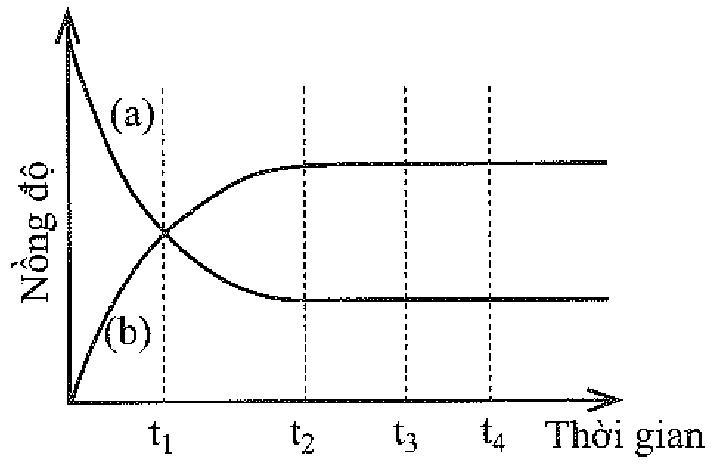
\includegraphics[width=\textwidth]{2025_10_23_f2823ef970776205e47bg-01}
\captionsetup{labelformat=empty}
\caption{Hình 1.1. Biến thiên nồng độ chất phản ứng và chất sản phẩm theo thời gian}
\end{center}
\end{figure}

\section*{Côt A}
a) Đường (a)\\
b) $t_{1}$\\
c) Dường (b)\\
d) $\mathrm{t}_{2}$

\section*{Cột B}
\begin{enumerate}
  \item không phải là thời điểm bắt đầu trạng thái cân bằng.
  \item mô tả biến thiên nồng độ chất sản phẩm theo thời gian.
  \item là thời điểm phản ứng đạt trạng thái cân bằng.
  \item mô tả biến thiên nồng độ chất phản ứng theo thòi gian.\\
1.3. Quan sát Hình 1.2 và chọn phát biểu đúng.
\end{enumerate}

\begin{figure}[h]
\begin{center}
  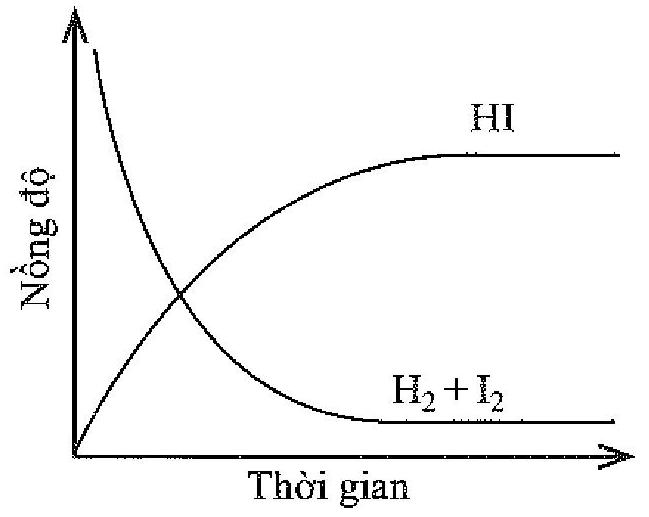
\includegraphics[width=\textwidth]{2025_10_23_f2823ef970776205e47bg-02(1)}
\captionsetup{labelformat=empty}
\caption{a)}
\end{center}
\end{figure}

\begin{figure}[h]
\begin{center}
  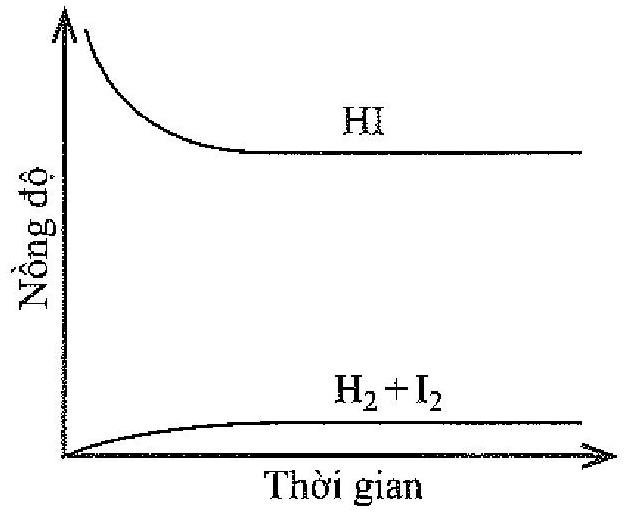
\includegraphics[width=\textwidth]{2025_10_23_f2823ef970776205e47bg-02}
\captionsetup{labelformat=empty}
\caption{b)}
\end{center}
\end{figure}

Himin 1.2\\
A. Cả hai đồ thị đều mô tả phản ứng đã đạt đến trạng thái cân bằng.\\
B. Cả hai đồ thị đều không mô tả phản ứng đã đạt đến trạng thái cân bằng.\\
C. Chỉ đồ thị (a) mô tả phản ứng đã đạt đến trạng thái cân bằng.\\
D. Chỉ đồ thị (b) mô tả phản ứng đã đạt đến trạng thái cân bằng.\\
1.4. Biểu thức nào sau đây là biểu thức hằng số cân bằng ( $\mathrm{K}_{\mathrm{C}}$ ) của phản ứng $\mathrm{C}(s)+2 \mathrm{H}_{2}(g) \rightleftharpoons \mathrm{CH}_{4}(g) ?$\\
A. $\mathrm{K}_{\mathrm{C}}=\frac{\left[\mathrm{CH}_{4}\right]}{\left[\mathrm{H}_{2}\right]}$.\\
B. $\mathrm{K}_{\mathrm{C}}=\frac{\left[\mathrm{CH}_{4}\right]}{[\mathrm{C}]\left[\mathrm{H}_{2}\right]^{2}}$.\\
C. $\mathrm{K}_{\mathrm{C}}=\frac{\left[\mathrm{CH}_{4}\right]}{[\mathrm{C}]\left[\mathrm{H}_{2}\right]}$.\\
D. $\mathrm{K}_{\mathrm{C}}=\frac{\left[\mathrm{CH}_{4}\right]}{\left[\mathrm{H}_{2}\right]^{2}}$.\\
1.5. Cho phản úng $\mathrm{A}(g) \rightleftharpoons \mathrm{B}(g)$. Hằng số cân bằng của phản ứng đâ cho là $\mathrm{K}_{\mathrm{C}}=1,0.10^{3}$. Tại trạng thái cân bằng, nồng độ của chất A là $1,0.10^{-3} \mathrm{M}$ thì nồng độ cân bằng của B là\\
A. $1,0.10^{-3} \mathrm{M}$.\\
B. $1,0 \mathrm{M}$.\\
C. $2,0 \mathrm{M}$.\\
D. $1,0.10^{3} \mathrm{M}$.\\
1.6. Xét cân bằng sau: $\mathrm{H}_{2}(g)+1_{2}(g)=2 \mathrm{HI}(g)$\\
a) Hãy hoàn thành bảng sau.

\begin{center}
\begin{tabular}{|l|l|l|l|l|}
\hline
Nhiêt đọ ( ${ }^{\circ} \mathrm{C}$ ) & $\left[\mathrm{H}_{2}\right]\left(\mathrm{mol} \mathrm{L}^{-1}\right)$ & $[1](\mathrm{mol} \mathrm{L})$ & [HI] (mol L-) & $\mathrm{K}_{\mathrm{c}}$ \\
\hline
25 & 0,0355 & 0,0388 & 0,9220 & ...(1)... \\
\hline
340 & ...(2)... & 0,0455 & 0,3870 & 9,6 \\
\hline
445 & 0,0485 & 0,0468 & ...(3)... & 50,2 \\
\hline
\end{tabular}
\end{center}

b*) Hãy cho biết khi nhiệt độ tăng thì cân bằng chuyển dịch theo chiều nào.\\
1.7. Phát biểu nào sau đây về phản ứng ở trạng thái cân bằng là không đúng?\\
A. Các phản ứng thuận và phản ứng nghịch diễn ra với tốc độ như nhau.\\
B. Nồng độ của chất phản ứng và chất sản phẩm không thay đổi.\\
C. Nồng độ của các chất phản ứng bằng nồng độ của các chất sản phẩm.\\
D. Các phản ứng thuận và nghịch tiếp tục xảy ra.\\
1.8. Xét cân bằng sau:

$$
2 \mathrm{SO}_{2}(g)+\mathrm{O}_{2}(g) \rightleftharpoons 2 \mathrm{SO}_{3}(g)
$$

Nếu tăng nồng độ $\mathrm{SO}_{2}(\mathrm{~g})$ (các điều kiện khác giữ không đổi), cân bằng sẽ chuyển dịch theo chiểu nào?\\
A. Chuyển dịch theo chiều nghịch.\\
B. Chuyển dịch theo chiều thuận.\\
C. Có thể chuyển dịch theo chiều thuận hoặc chiều nghịch tuỳ thuộc vào lượng $\mathrm{SO}_{2}$ thêm vào.\\
D. Không thay đồi.\\
1.9*. Xét cân bằng sau diễn ra trong một piston ở nhiệt độ không đổi:

$$
\mathrm{N}_{2}(g)+3 \mathrm{H}_{2}(g) \rightleftharpoons 2 \mathrm{NH}_{3}(g)
$$

Nếu nén piston thì cân bằng sẽ chuyển dịch theo chiều nào?\\
A. Chuyển dịch theo chiểu nghịch.\\
B. Chuyển dịch theo chiều thuận.\\
C. Có thể chuyển dịch theo chiều thuận hoặc chiều nghịch tuỳ thuộc vào piston bị nén nhanh hay chậm.\\
D. Không thay đồi.\\
1.10. Đối với phản ứng sau, cân bằng sẽ bị ảnh hưởng như thế nào khi tăng nhiệt độ (các điều kiện khác giữ không đổi)?

$$
\mathrm{H}_{2}(g)+\frac{1}{2} \mathrm{O}_{2}(g)=\mathrm{H}_{2} \mathrm{O}(l) \quad \Delta_{\mathrm{r}} \mathrm{H}_{298}^{\circ}=-286 \mathrm{~kJ}
$$

A. Cân bằng chuyển dịch sang phải.\\
B. Cân bằng chuyển dịch sang trái.\\
C. Không thay đổi.\\
D. Không dự đoán được sự chuyển dịch cân bằng.\\
1.11. Trong phản úng nào sau đây sự tăng áp suất sẽ dẫn tới cân bằng chuyển dịch sang trái (các điều kiện khác coi như không thay đồi)?\\
A. $\mathrm{CaCO}_{3}(s)=\mathrm{CaO}(s)+\mathrm{CO}_{2}(g)$\\
B. $\mathrm{CO}(g)+\mathrm{H}_{2} \mathrm{O}(g) \rightleftharpoons \mathrm{H}_{2}(g)+\mathrm{CO}_{2}(g)$\\
C. $2 \mathrm{H}_{2}(g)+\mathrm{O}_{2}(g) \rightleftharpoons 2 \mathrm{H}_{2} \mathrm{O}(l)$\\
D. $\mathrm{C}(s)+\mathrm{O}_{2}(g) \rightleftharpoons \mathrm{CO}_{2}(g)$\\
1.12. Viết biểu thức hằng số cân bằng cho các phản ưng dưới đây:\\
a) $2 \mathrm{Hg}(l)+\mathrm{O}_{2}(g) \rightleftharpoons 2 \mathrm{HgO}(s)$\\
b) $\mathrm{CH}_{3} \mathrm{COOH}(a q)+\mathrm{C}_{2} \mathrm{H}_{5} \mathrm{OH}(a q)=\mathrm{CH}_{3} \mathrm{COOC}_{2} \mathrm{H}_{5}(a q)+\mathrm{H}_{2} \mathrm{O}(l)$\\
c) $\mathrm{CO}(g)+\mathrm{H}_{2} \mathrm{O}(g) \rightleftharpoons \mathrm{H}_{2}(g)+\mathrm{CO}_{2}(g)$\\
d) $2 \mathrm{FeCl}_{3}(s) \rightleftharpoons 2 \mathrm{FeCl}_{2}(s)+\mathrm{Cl}_{2}(g)$\\
1.13. Xét phản úng: $\quad \mathrm{H}_{2}(g)+\mathrm{I}_{2}(g)=2 \mathrm{HI}(g)$

Một hỗn hợp phản ứng chưa trong bình dung tích 3,67 lít ở một nhiệt độ nhất định; ban đầu chứa 0,763 gam $\mathrm{H}_{2}$ và 96,9 gam $\mathrm{I}_{2}$. Ờ trạng thái cân bằng, bình chứa 90,4 gam HI. Tính hằng số cân bằng ( $\mathrm{K}_{\mathrm{C}}$ ) cho phản ứng ở nhiệt độ này.\\
1.14*. Lượng đường glucose trong máu người thường ổn định ở nồng độ khoảng $0,1 \%$. Khi ta ăn tinh bột, glucose sẽ được sinh ra trong cơ thể; còn khi cơ thể vận động và hoạt động trí não, glucose bị tiêu thụ.\\
a) Em hãy tìm hiểu để giải thích vì sao lượng glucose trong máu luôn ổn định ở mức khoảng $0,1 \%$.\\
b) Theo em, khi cơ thể hoạt động thể thao hay khi ăn uống sẽ xảy ra đồng thời hai quá trình sinh ra và mất đi glucose? Giải thích. Sự ổn định của glucose trong máu có thể được coi là trạng thái cân bằng hoá học không? Nếu có, hãy đề xuất cân bằng đó.\\
1.15. Carbon monoxide thay thế oxygen trong hemoglobin đã bị oxi hoá theo phản ứng: $\quad \mathrm{HbO}_{2}(a q)+\mathrm{CO}(a q) \rightleftharpoons \mathrm{HbCO}(a q)+\mathrm{O}_{2}(a q)$\\
Tại nhiệt độ trung bình trong cơ thể, hằng số cân bằng của phản ứng trên là $K_{C}=170$.\\
Giả sử một hỗn hợp không khí bị ô nhiễm carbon monoxide ở mực $0,1 \%$ (theo thể tích). Coi không khí chứa $20,0 \%$ oxygen về thể tích; tî lệ oxygen và carbon monoxide hoà tan trong máu giống với tỉ lệ của chúng trong không khí. Cho biết tỉ lệ HbCO so với $\mathrm{HbO}_{2}$ trong máu là bao nhiêu. Em có nhận xét gì về tính độc của khí CO ?

\section*{BT SU. DICAN LI TRONG DUNG DICH NUÓC. THUYÉT BRONSTED - LOWRY VỂ ACD - BASE}
2.1. Diền từ ngữ thích hợp vào chỗ trống trong mỗi phát biểu sau:\\
a) Quá trình phân li của các chất khi tan trong nước thành các ion được gọi là ... (1)... Chất điện li là chất khi tan trong nước phân li thành các ... (2)....\\
... (3)... là chất khi tan trong nước không phân li thành các ion.\\
b) Theo thuyết Bronsted - Lowry, ...(1)... là những chất có khả năng cho $\mathrm{H}^{+}$, ... (2) ... là những chất có khả năng nhận $\mathrm{H}^{+}$. Acid mạnh và base mạnh phân li ... (3) ... trong nước; acid yếu và base yếu phân li ... (4)... trong nước.\\
2.2 Cho các chất: $\mathrm{NaOH}, \mathrm{HCl}, \mathrm{HNO}_{3}, \mathrm{NaNO}_{3}$, saccharose ( $\mathrm{C}_{12} \mathrm{H}_{22} \mathrm{O}_{11}$ ), ethanol, glycerol, $\mathrm{KAl}\left(\mathrm{SO}_{4}\right)_{2} \cdot 12 \mathrm{H}_{2} \mathrm{O}$. Trong các chất trên, có bao nhiêu chất tạo được dung dịch dẫn điện?\\
A. 5 .\\
B.3.\\
C. 6 .\\
D. 2 .\\
2.3. Phương trình mô tả sự điện li của NaCl trong nước là\\
A. $\mathrm{NaCl}(s) \xrightarrow{\mathrm{H}_{2} \mathrm{O}} \mathrm{Na}(a q)+\mathrm{Cl}(a q)$\\
B. $\mathrm{NaCl}(s) \xrightarrow{\mathrm{H}_{2} \mathrm{O}} \mathrm{Na}^{+}(g)+\mathrm{Cl}^{-}(g)$\\
C. $\mathrm{NaCl}(s) \xrightarrow{\mathrm{H}_{2} \mathrm{O}} \mathrm{Na}^{+}(a q)+\mathrm{Cl}^{-}(a q)$\\
D. $\mathrm{NaCl}(s) \xrightarrow{\mathrm{H}_{2} \mathrm{O}} \mathrm{Na}(s)+\mathrm{Cl}(s)$\\
2.4. Phương trình mô tả sự điện li của $\mathrm{Na}_{2} \mathrm{CO}_{3}$ trong nước là\\
A. $\mathrm{Na}_{2} \mathrm{CO}_{3}(s) \xrightarrow{\mathrm{H}_{2} \mathrm{O}} 2 \mathrm{Na}(a q)+\mathrm{C}(a q)+3 \mathrm{O}(a q)$\\
B. $\mathrm{Na}_{2} \mathrm{CO}_{3}(s) \xrightarrow{\mathrm{H}_{2} \mathrm{O}} 2 \mathrm{Na}^{+}(a q)+\mathrm{C}^{4+}(a q)+3 \mathrm{O}^{2-}(a q)$\\
C. $\mathrm{Na}_{2} \mathrm{CO}_{3}(s) \xrightarrow{\mathrm{H}_{2} \mathrm{O}} 2 \mathrm{Na}^{+}(a q)+\mathrm{CO}_{3}^{2-}(a q)$\\
D. $\mathrm{Na}_{2} \mathrm{CO}_{3}(s) \xrightarrow{\mathrm{H}_{2} \mathrm{O}} 2 \mathrm{Na}^{+}(s)+\mathrm{CO}_{3}^{2-}(g)$\\
2.5. Ở cùng nồng độ và cùng điều kiện, chất nào sau đây tạo ra nhiều ion $\mathrm{H}^{+} \left(\mathrm{H}_{3} \mathrm{O}^{+}\right)$nhất trong dung dịch?\\
A. Acid mạnh.\\
B. Base manh.\\
C. Acid yếu.\\
D. Nước.\\
2.6. Đặc điểm nào sau đây là không đúng khi mô tả về acid mạnh?\\
A. Phân li hoàn toàn trong nước.\\
B. Dung dịch nước của chúng dẫn điện.\\
C. Có khả năng nhận $\mathrm{H}^{+}$.\\
D. Có khả năng cho $\mathrm{H}^{+}$.\\
2.7. Đặc điểm nào sau đây là không đúng khi mô tả về base yếu?\\
A. Trong dung dịch nước, không phân li hoàn toàn ra $\mathrm{OH}^{-}$.\\
B. Có khả năng nhận $\mathrm{H}^{+}$.\\
C. Dung dịch nước của chúng dẫn điện.\\
D. Co khà năng cho $\mathrm{H}^{+}$.\\
2.8. Trong phản ứng sau đây, những chất nào đóng vai trò là acid theo thuyết Bronsted - Lowry?

$$
\mathrm{H}_{2} \mathrm{~S}(a q)+\mathrm{H}_{2} \mathrm{O} \rightleftharpoons \mathrm{HS}^{-}(a q)+\mathrm{H}_{3} \mathrm{O}^{+}(a q)
$$

A. $\mathrm{H}_{2} \mathrm{~S}$ và $\mathrm{H}_{2} \mathrm{O}$.\\
B. $\mathrm{H}_{2} \mathrm{~S}$ và $\mathrm{H}_{3} \mathrm{O}^{+}$.\\
C. $\mathrm{H}_{2} \mathrm{~S}$ và HS .\\
D. $\mathrm{H}_{2} \mathrm{O}$ và $\mathrm{H}_{3} \mathrm{O}^{+}$.\\
2.9. Trong phản ứng sau đây, những chất nào đóng vai trò là base theo thuyết Brønsted - Lowry?

$$
\mathrm{CO}_{3}^{2-}(a q)+\mathrm{H}_{2} \mathrm{O} \rightleftharpoons \mathrm{HCO}_{3}^{-}(a q)+\mathrm{OH}^{-}(a q)
$$

A. $\mathrm{CO}_{3}^{2-}$ và $\mathrm{OH}^{-}$.\\
B. $\mathrm{CO}_{3}^{2-}$ và $\mathrm{HCO}_{3}^{-}$.\\
C. $\mathrm{H}_{2} \mathrm{O}$ và $\mathrm{OH}^{-}$.\\
D. $\mathrm{H}_{2} \mathrm{O}$ và $\mathrm{CO}_{3}^{2-}$.\\
2.10. Base liên hợp của các acid $\mathrm{HCOOH}, \mathrm{HCl}, \mathrm{NH}_{4}^{+}$lần lượt là\\
A. $\mathrm{HCOO}, \mathrm{Cl}^{-}, \mathrm{NH}_{3}$.\\
B. $\mathrm{COO}^{2-}, \mathrm{Cl}^{-}, \mathrm{NH}_{2}^{-}$.\\
C. $\mathrm{HCOO}^{-}, \mathrm{Cl}^{-}, \mathrm{NH}_{2}^{-}$.\\
D. $\mathrm{HCOO}^{-}, \mathrm{Cl}, \mathrm{NH}_{2}$.\\
2.11. Cho phản úng: $\mathrm{H}_{2} \mathrm{SO}_{4}(a q)+\mathrm{H}_{2} \mathrm{O}(a q) \rightarrow \mathrm{HSO}_{4}^{-}(a q)+\mathrm{H}_{3} \mathrm{O}^{+}(a q)$ Cặp acid - base liên hợp trong phản ứng trên là:\\
A. $\mathrm{H}_{2} \mathrm{SO}_{4}$ và $\mathrm{HSO}_{4}^{-}$.\\
B. $\mathrm{H}_{2} \mathrm{O}$ và $\mathrm{H}_{3} \mathrm{O}^{+}$.\\
C. $\mathrm{H}_{2} \mathrm{SO}_{4}$ và $\mathrm{SO}_{4}^{2-} ; \mathrm{H}_{2} \mathrm{O}$ và $\mathrm{OH}^{-}$.\\
D. $\mathrm{H}_{2} \mathrm{SO}_{4}$ và $\mathrm{HSO}_{4}^{-} ; \mathrm{H}_{3} \mathrm{O}^{+}$và $\mathrm{H}_{2} \mathrm{O}$.\\
2.12. Viết phương trình điện li trong nước của các chất sau: $\mathrm{NaHCO}_{3}, \mathrm{CuCl}_{2}$, $\left(\mathrm{NH}_{4}\right)_{2} \mathrm{SO}_{4}, \mathrm{Fe}\left(\mathrm{NO}_{3}\right)_{3}$.\\
2.13. Sodium hydroxide ( NaOH ) là một chất điện li mạnh, trong khi methanol $\left(\mathrm{CH}_{3} \mathrm{OH}\right)$ là chất không điện li. Hãy mô tả sự khác nhau khi hoà tan các chất trên vào nước. Viết các phương trình minh hoạ.\\
2.14. Viết dạng tồn tại chủ yếu trong dung dịch nước của các chất theo bảng sau đây.

\begin{center}
\begin{tabular}{|l|l|l|}
\hline
Chát & Dace diem & Dang tón rai chú yêu trong dung dieh nurfe \\
\hline
$\mathrm{CH}_{3} \mathrm{COOH}$ & Acid yếu &  \\
\hline
$\mathrm{HNO}_{3}$ & Acid mạnh &  \\
\hline
$\mathrm{C}_{6} \mathrm{H}_{12} \mathrm{O}_{6}$ (glucose) & Chất không điện li &  \\
\hline
NaOH & Base manh &  \\
\hline
\end{tabular}
\end{center}

2.15. "Ợ nóng" là cảm giác đau rát ở thực quản gây ra do sự gia tăng nồng độ hydrochloric acid $(\mathrm{HCl})$ trong dạ dày.\\
a) Cách đơn giản nhất để giảm chứng ợ nóng nhẹ là nuốt nước bọt nhiều lần do nước bọt có chứa ion bicarbonate ( $\mathrm{HCO}_{3}^{-}$), hoạt động như một base, khi nuốt vào sẽ trung hoà một phần acid trong thực quản. Viết phưong trình hoá học của phản úng giữa HCl và $\mathrm{HCO}_{3}^{-}$.\\
b) Có thể điều trị chứng ợ nóng bằng cách sử dụng các thuốc kháng acid, chẳng hạn "sữa magie" có thành phần chủ yếu là huyền phù $\mathrm{Mg}(\mathrm{OH})_{2}$. Hãy viết phương trình hoá học của phản ứng giữa HCl và $\mathrm{Mg}(\mathrm{OH})_{2}$; giải thích vì sao "sữa magie" hiệu quả hơn nước bọt trong việc trung hoà acid thực quản.\\
2.16. Hiện nay, năng lượng mà con người sử dụng trong đời sống và sản xuất chủ yếu lấy từ quá trình đốt cháy các nhiên liệu hoá thạch như xăng, dầu, khí đốt tự nhiên và than đá. Một số nhiên liệu hoá thạch, đặc biệt là than đá, có chứa một lượng nhỏ tạp chất sulfur (lưu huỳnh). Trong quá trình đốt cháy, các tạp chất này phản ứng với oxygen tạo thành sulfur dioxide ( $\mathrm{SO}_{2}$ ). Ngoài ra, trong quá trình đốt cháy bất kì nhiên liệu hoá thạch nào, nitrogen từ không khí phản ứng với oxygen tạo thành nitrogen dioxide ( $\mathrm{NO}_{2}$ ). Sulfur dioxide và nitrogen dioxide phản ứng với nước và oxygen ( $\mathrm{O}_{2}$ ) trong khi quyển để tạo thành sulfuric acid và nitric acid:

$$
\begin{aligned}
& 2 \mathrm{SO}_{2}+\mathrm{O}_{2}+2 \mathrm{H}_{2} \mathrm{O} \rightarrow 2 \mathrm{H}_{2} \mathrm{SO}_{4} \\
& 4 \mathrm{NO}_{2}+\mathrm{O}_{2}+2 \mathrm{H}_{2} \mathrm{O} \rightarrow 4 \mathrm{HNO}_{3}
\end{aligned}
$$

Các acid này kết hợp với nước mưa tạo thành mưa acid. Hãy viết phương trình điện li của $\mathrm{H}_{2} \mathrm{SO}_{4}$ và $\mathrm{HNO}_{3}$ trong nước, biết rằng $\mathrm{H}_{2} \mathrm{SO}_{4}$ diện li theo hai nấc, trong đó nấc thứ nhất điện li hoàn toàn tạo thành $\mathrm{HSO}_{4}^{-}$và $\mathrm{HSO}_{4}^{-}$ điện li không hoàn toàn ở nấc thứ hai.\\
3.1. Diền thông tin thích hợp vào chỗ trống trong mỗi câu dưới đây.

Ở $25^{\circ} \mathrm{C},\left[\mathrm{H}^{+}\right]\left[\mathrm{OH}^{-}\right]=\ldots$ (1) $\ldots$ luôn đúng đối với các dung dịch nước. Khi $\left[\mathrm{H}^{+}\right] \ldots$ (2) $\ldots 1,0.10^{-7} \mathrm{M}$ thì dung dịch có tính acid; khi $\left[\mathrm{H}^{+}\right]$nhỏ hon $\ldots$ (3) $\ldots$ thì dung dịch có tính base; khi $\left[\mathrm{H}^{+}\right]=1,0.10^{-7} \mathrm{M}$, dung dịch $\ldots$ (4) $\ldots$. Dung dịch acid có ... (5) ... nhỏ hơn $1,0.10^{-7} \mathrm{M}$, dung dịch base có $\left[\mathrm{OH}^{-}\right]$lớn hơn $\ldots$ (6) ... và dung dịch trung tính có $\left[\mathrm{OH}^{-}\right]=\ldots$ (7) ....\\
3.2. Những phát biểu nào dưới đây là đúng?\\
(a) Để so sánh mức độ acid giữa các dung dịch có thể dựa vào nồng đọ: dung dịch acid nào có nồng độ lớn hon sẽ có tính acid mạnh hon.\\
(b) Trong các dung dịch có cùng nồng độ, dung dịch nào có tính acid mạnh hơn sẽ có nồng độ ion $\mathrm{H}^{+}$lớn hơn và pH lớn hơn.\\
(c) Trong các đung dịch có cùng nồng đọ, dung dịch nào có nồng độ ion $\mathrm{OH}^{-}$ lớn hơn và pH nhỏ hơn sẽ có tính base lớn hon.\\
(d) Trong các dung dịch có cùng nồng độ, dung dịch nào có tính acid mạnh hơn sẽ có nồng độ ion $\mathrm{H}^{+}$lón hơn và pH nhỏ hơn.\\
(e) Trong các dung dịch có cùng nồng độ, dung dịch có nồng độ ion $\mathrm{H}^{+}$nhỏ và pH cao sẽ có tính acid yếu hon.\\
(g) Trong một dãy các dung dịch có cùng nồng độ được sắp xếp theo tính acid tăng dần thì nồng độ ion $\mathrm{OH}^{-}$sẽ giảm dần và $\mathrm{K}_{\mathrm{a}}$ tăng dần.\\
3.3. Nối các đặc điểm ở cột A với chiều thay đổi tính acid, base tương úng ở cột B cho phù hợp.

\section*{CôtA}
a) Nồng độ ion $\mathrm{OH}^{-}$giảm dần\\
b) pH tăng dần\\
c) Nồng độ ion $\mathrm{H}^{+}$tăng dần\\
d) Nồng độ ion $\mathrm{H}^{+}$giảm dần\\
e) pH giàm dần\\
g) Nồng độ ion $\mathrm{OH}^{-}$tăng dần

\section*{Côt B}
\begin{enumerate}
  \item Tính acid tăng dần
  \item Tính base tăng dần
\end{enumerate}

Đề xuất cách có thể thực hiện để làm tăng tính acid hoặc làm tăng tính base của dung dịch từ dung dịch trung tính. Bằng cách nào để có thể biết được tinh acid hoặc tính base tăng lên?\\
3.4. Một dung dịch có $\mathrm{pH}=11,7$. Nồng độ ion hydrogen $\left(\mathrm{H}^{+}\right)$của dung dịch là\\
A. $2,3 \mathrm{M}$.\\
B. $11,7 \mathrm{M}$.\\
C. $5,0.10^{-3} \mathrm{M}$.\\
D. $2,0,10^{-12} \mathrm{M}$.\\
3.5. Giá trị pH của một dung dịch tăng từ 3 lên 5. Những nhận định nào sau đây là sai?\\
(a) Nồng độ ion $\mathrm{H}^{+}$của đủng dịch giảm 20 lần.\\
(b) Nồng độ ion $\mathrm{OH}^{-}$của dung dịch khi $\mathrm{pH}=5$ là $10^{-9} \mathrm{M}$.\\
(c) Nồng độ ion $\mathrm{H}^{+}$của đung dịch khi $\mathrm{pH}=3$ là $10^{-3} \mathrm{M}$.\\
(d) Dung dịch ban đầu là một acid có nồng độ $0,001 \mathrm{M}$.\\
(e) Dung dịch ban đầu là một base có nồng độ $0,001 \mathrm{M}$.\\
3.6. Calcium hydroxide rắn được hoà tan trong nước cho tới khi pH của dung dịch đạt 10,94 . Nồng độ của ion hydroxide $\left(\mathrm{OH}^{-}\right)$trong dung dịch là\\
A. $1,1.10^{-11} \mathrm{M}$.\\
B. $3,06 \mathrm{M}$.\\
C. $8,7,10^{-4} \mathrm{M}$.\\
D. $1,0.10^{-14} \mathrm{M}$.\\
3.7*. Bảng dưới đây là kết quả đo pH của các dung dịch bằng máy đo pH . Xác định tính acid, base hay trung tính và màu của giấy chỉ thị pH khi dùng để thử vào hai cột còn trống trong bảng dưới đây.

\begin{center}
\begin{tabular}{|l|l|l|l|}
\hline
During dich & pH & Timh acid, base hay trung tinh & Man cúa giáy chi thi pH \\
\hline
A & 1 &  &  \\
\hline
B & 11 &  &  \\
\hline
C & 7 &  &  \\
\hline
D & 3 &  &  \\
\hline
E & 13 &  &  \\
\hline
F & 9 &  &  \\
\hline
\end{tabular}
\end{center}

3.8. Một dung dịch X thu được bằng cách thêm $50,0 \mathrm{~mL}$ dung dịch $\mathrm{HBr} 0,050 \mathrm{M}$ vào $150,0 \mathrm{~mL}$ dung dịch $\mathrm{HI} 0,100 \mathrm{M}$. Tính nồng độ $\mathrm{H}^{+}$và pH của dung dịch X . Biết HBr và HI đều được coi là acid mạnh.\\
3.9. Xác định pH của dung dịch thu được sau khi thêm $25,0 \mathrm{~mL}$ dung dịch NaOH $0,1 \mathrm{M}$ vào $50,0 \mathrm{~mL}$ dung dịch $\mathrm{HCl} 0,1 \mathrm{M}$.\\
3.10. Ở $25^{\circ} \mathrm{C}, \mathrm{pH}$ của một dung dịch $\mathrm{Ba}(\mathrm{OH})_{2}$ là 10,66 . Nồng độ ion hydroxide $\left(\mathrm{OH}^{-}\right)$trong dung dịch là bao nhiêu? Để thu được 125 mL dung dịch $\mathrm{Ba}(\mathrm{OH})_{2}$ trên thì khối lượng $\mathrm{Ba}(\mathrm{OH})_{2}$ cần phải hoà tan là bao nhiêu (bỏ qua sự thay đổi thể tích nếu có)?\\
3.11. Cho ba dung dịch có cùng nồng đọ: hydrochloric acid $(\mathrm{HCl})$, ethanoic acid (acetic acid, $\mathrm{CH}_{3} \mathrm{COOH}$ ) và sodium hydroxide ( NaOH ). Khi chuẩn độ riêng một thể tích như nhau của dung dịch HCl và dung dịch $\mathrm{CH}_{3} \mathrm{COOH}$ bằng dung dịch NaOH , phát biểu nào sau đây là đúng?\\
A. Trước khi chuẩn độ, pH của hai acid bằng nhau.\\
B. Tại các điểm tương đương, dung dịch của cả hai phép chuẩn độ đều có giá trị pH bằng 7 .\\
C. Cần cùng một thể tích sodium hydroxide để đạt đến điểm tương đương.\\
D. Giá trị pH của hai acid tăng như nhau cho đến khi đạt điểm tương đương.\\
3.12. a) Cốc A chứa 50 mL dung dịch $\mathrm{KOH} 0,10 \mathrm{M}$ được chuẩn độ với dung dịch $\mathrm{HNO}_{3} 0,10 \mathrm{M}$. Sau khi thêm 52 mL dung dịch $\mathrm{HNO}_{3}$ vào, pH của dung dịch trong cốc Alà\\
A. 2,80 .\\
B. 2,71 .\\
C. 2,40 .\\
D. 3,00 .\\
b) Chuẩn độ $100,0 \mathrm{~mL}$ dung dịch $\mathrm{NaOH} 0,1 \mathrm{M}$ bằng dung dịch $\mathrm{HCl} 1,0 \mathrm{M}$. Thể tích dung dịch HCl cần thêm để dung dịch thu được có $\mathrm{pH}=12$ là\\
A. $8,91 \mathrm{~mL}$.\\
B. $8,52 \mathrm{~mL}$.\\
C. $9,01 \mathrm{~mL}$.\\
D. $8,72 \mathrm{~mL}$.\\
3.13. Một mẫu dung dịch $\mathrm{H}_{2} \mathrm{SO}_{4}$ (gọ là mẫu A ) được phân tích bằng cách thêm $50,0 \mathrm{~mL}$ dung dịch $\mathrm{NaOH} 0,213 \mathrm{M}$ vào 100 mL dung dịch mẫu A rồi lắc đều. Sau khi phản ứng xảy ra, người ta thấy trong hỗn hợp dung dịch còn dư ion $\mathrm{OH}^{-}$. Phần ion dư này cần $13,21 \mathrm{~mL} \mathrm{HCl} 0,103 \mathrm{M}$ để trung hoà. Tính nồng độ $\mathrm{mol} \mathrm{L}^{-1}$ của mẫu A .\\
3.14. a) Lan thực hiện phép chuẩn độ $50,00 \mathrm{~mL}$ dung dịch acid nồng độ $0,10 \mathrm{M}$ bằng dung dịch NaOH cùng nồng độ ( $0,10 \mathrm{M}$ ), Lan rất ngạc nhiên khi thấy phải cần 100 mL dung dịch NaOH để đạt tới điểm tương đương. Em hãy giải thích thắc mắc cho Lan.\\
b) Trong một thí nghiệm khác, Lan thực hiện chuẩn độ $10,00 \mathrm{mLHCl} 0,020 \mathrm{M}$. Một lần nữa, Lan rất ngạc nhiên khi chỉ cẩn $5,00 \mathrm{~mL}$ một base mạnh cùng nồng độ $0,020 \mathrm{M}$ để phản ứng hoàn toàn với $10,00 \mathrm{~mL} \mathrm{HCl}$ đó. Em hãy giải thích cho Lan vì sao không cần một lượng tương đương là $10,00 \mathrm{~mL}$ base mà chỉ cần $5,00 \mathrm{~mL}$ ?\\
$3.15^{*}$ a) 10 mL dung dịch sulfuric acid $5.10^{-3} \mathrm{M}$ được cho vào một bình định mức dung tích 100 mL .\\
a1) Tính pH của dung dịch sulfuric acid (cho rằng $\mathrm{H}_{2} \mathrm{SO}_{4}$ là acid mạnh phân li trong nước hoàn toàn cả hai proton $\mathrm{H}^{+}$).\\
a2) Thêm nước vào đến vạch của bình định mức thu được 100 mL dung dịch. Xác định pH của dung dịch đã pha loãng.\\
b) Viết phương trình hoá học của phản ứng giữa sulfuric acid với đung dịch sodium hydroxide.\\
c) Dung dịch pha loãng ở phần a2 được dùng để chuẩn độ $25,0 \mathrm{~mL}$ dung dịch sodium hydroxide $1,00.10^{-4} \mathrm{M}$.\\
c1) Dư đoán hiện tượng quan sát được khi chuẩn độ đạt đến điểm tương đương nếu dùng phenolphthalein làm chất chỉ thị cho phép chuẩn độ trên.\\
c2) Xác định thể tích acid cần dùng khi phép chuẩn độ kết thúc.\\
3.16*. Nồng độ carbon dioxide ( $\mathrm{CO}_{2}$ ) trong khí quyển đã tăng khoảng $20 \%$ trong thế kỉ qua. Giả sử các đại dương của Trái Đất tiếp xúc với khí $\mathrm{CO}_{2}$ trong khí quyển, lượng $\mathrm{CO}_{2}$ tăng lên có thể có ảnh hưởng gì đến pH của các đại dương trên thế giới? Sự thay đổi này có thể ảnh hưởng gì đến cấu trúc đá vôi (chủ yếu là $\mathrm{CaCO}_{3}$ ) của các rạn san hô và vó sò biển?\\
3.17*. Oxygen được dẫn truyền trong cơ thể là do khả năng liên kết của oxygen với hồng cầu trong máu theo cân bằng sau:

$$
\mathrm{HbH}^{+}(a q)+\mathrm{O}_{2}(a q) \rightleftharpoons \mathrm{HbO}_{2}(a q)+\mathrm{H}^{+}(a q)
$$

Độ pH của máu người bình thường được kiểm soát chặt chẽ trong khoảng $7,35-7,45$. Dựa vào cân bằng trên, giải thích vì sao việc kiểm soát pH của máu người lại quan trọng. Diều gl̉ sẽ xảy ra với khả năng vận chuyển oxygen của hồng cầu nếu máu trở nên quá acid (một tình trạng nguy hiểm được gọi là nhiễm toan hay nhiễm độc acid)?\\
3.18. Acetic acid $\left(\mathrm{CH}_{3} \mathrm{COOH}\right)$ là một acid yếu.\\
a) Thế nào là một acid yếu? Viết phương trình hoá học của phản ứng giữa acetic acid với nước.\\
b) Giải thích vì sao giấm ăn (thành phần chính là acetic acid) thường được dùng để làm sạch cặn bám ở đáy ấm đun nước hoặc phích nước được dùng để chứa nước sôi.

\section*{CHỦ DỀ 2 NITROGEN VÀ SULFUR}
\section*{Bis 4. DON CHÁT NITROGEN}
4.1. Phát biểu nào sau đây về nguyên tố nitrogen ( ${ }_{7} \mathrm{~N}$ ) là không đúng?\\
A. Nguyên tữ nguyên tố nitrogen có cấu hình electron là $1 \mathrm{~s}^{2} 2 \mathrm{~s}^{2} 2 \mathrm{p}^{3}$.\\
B. Nguyên tữ nguyên tố nitrogen có 3 electron hoá trị.\\
C. Nguyên tố nitrogen thuộc chu kì 2 , nhóm VA trong bảng tuần.\\
D. Trong một số họp chất, nguyên tử nitrogen có thể dùng cặp electron hoá trị riêng để tạo một liên kết cho - nhận với nguyên tử khác.\\
4.2. Số oxi hoá và hoá trị của nitrogen trong hợp chất nitric acid lần lượt là:\\
A. +5 và V .\\
B. +5 và IV.\\
C. +5 và III.\\
D. +4 và IV.\\
4.3. Phát biểu nào sau đây về đơn chất nitrogen ( $\mathrm{N}_{2}$ ) là không đúng?\\
A. Dừ phân tữ $\mathrm{N}_{2}$ có tính kém hoạt động hoá học, nhưng vẫn hoạt động hoá học mạnh hơn chlorine, $\mathrm{Cl}_{2}$.\\
B. Đơn chất nitrogen không phản ưng với hydrogen, oxygen ở điều kiện thường.\\
C. Do có nhiệt độ rất thấp nên nitrogen lỏng được sử dụng bảo quản một số loại mẫu vật.\\
D. Trong bầu khí quyển, khi có sấm chớp, khí nitrogen tạo các nitrogen oxide, là một nguyên nhân làm cho nước mưa có tính acid.\\
4.4. Trong một số nghiên cứu tổng hợp hữu cơ cần môi trường trơ, người ta loại oxygen ra khỏi hệ phản ứng bằng cách dùng bơm chân không rút không khí ra khỏi hệ, sau đó xả khí nitrogen vào hệ phản ứng. Lượng khú được rút ra thường đi kèm một lượng dung môi hữu co, để tránh làm hỏng bơn và ngăn hơi dung môi hữu cơ độc hại thoát ra ngoài, lượng khí rút ra được dẫn qua bình chưa, bình này lại được ngâm trong nitrogen lỏng. Bình chưa này còn được gọi là bẫy dung môi, hơi dung môi sê bị giữ lại ở đây và được thu hồi sau khi phản ứng kết thúc. Nhiều nghiên cưu đã cho thấy, bẫy dung môi này tiềm ẩn nhiều nguy cơ phát nổ và thực tế đã không ít vụ nổ đã xảy ra. Nguyên nhân được cho là do sự gia tăng áp suất đột ngột khi oxygen lỏng bay hơi khi loại bỏ nitrogen lỏng cưng như phản ứng mãnh liệt giữa chất lỏng này với một số chất hữu cơ tạo thành các hợp chất dễ gây nổ.\\
(Nguồn: \href{https://researchsafety.northwestern.edu/safety-information/glass-vacuum-trap-safety-}{https://researchsafety.northwestern.edu/safety-information/glass-vacuum-trap-safety-}

Đọc đoạn thông tin trên và trả lờ các câu hỏi dưới đây bằng cách chọn phương án đúng:\\
a) Vai trò của khí nitrogen trong hệ phản ưng trên là gi?\\
A. Tạo môi trừng tro.\\
B. Là chất tham gia phản ứng.\\
C. Giữ nhiệt độ phản ứng cố định.\\
D. Hạn chế sự bay hơi của dung môi hữu co.\\
b) Có thể thay khí nitrogen bằng loại khí nào sau đây?\\
A. Các khí có chưa nguyên tố nitrogen vì nitrogen cần cho phản úng.\\
B. Hơi nước vì hơi nước giúp ổn định nhiệt độ và không độc hại.\\
C. Argon, neon, . . . hoặc các khí tro khác.\\
D. Các khí có tỉ trọng lớn để ngăn dung môi hữu cơ bay hơi.\\
c) Vì sao bẫy dung môi cần đươc ngâm trong nitrogen lóng?\\
A. Do nhiệt độ nitrogen long rất thấp.\\
B. Do phản ứng cần môi trường tro.\\
C. Dể hạ nhiệt độ phản ứng làm mát bơm.\\
D. Vì nitrogen lỏng có thể phản ứng với dung môi hữu cơ tạo chất ít độc hại.\\
d) Từ tìm hiểu, tra cứu nhiệt độ nóng chảy và nhiệt độ sôi của một số dung môi hữu cơ thông dụng, dự đoán dung môi hữu cơ được giữ lại trong bẫy dung môi dưới dạng nào sau đây.\\
A. Khí.\\
B. Lỏng.\\
C. Rắn.\\
D. Lỏng hoặc rắn.\\
e) Vì sao có sự xuất hiện của oxygen lỏng trong trong bẫy dung môi?\\
A. Oxygen có sẵn trong hệ khi rút ra sẽ hoá lỏng khi đi qua bẫy dung môi.\\
B. Nhiệt độ nóng chảy của oxygen cao hơn nhiệt độ nitrogen lỏng.\\
C. Oxygen được sinh ra trong phản ứng tổng hợp.\\
D. Oxygen có thể đi vào hệ thông qua các kẽ hở.\\
g) Nguyên nhân gây nổ được xác định là do oxygen lỏng. Để hạn chế việc này xảy ra người ta đă thiết kế, cải tiến bẫy dung môi bằng chất liệu phù hợp. Theo em, nên chọn loại vật liệu nào sau đây?\\
A. Loại thép dày, nếu vụ nổ có xảy ra cũng không thể phá huỷ, không gây nguy hiểm cho người sử dụng.\\
B. Vật liệu chống cháy, vụ nổ có thể tạo ra nhiều nhiệt do đó cần vật liệu cách nhiệt để tránh hơi nóng thoát ra gây hoả hoạn.\\
C. Thuỷ tinh cách nhiệt, trong suốt giúp quan sát phát hiện màu xanh của oxygen lỏng, đồng thời ngăn nhiệt thoát ra ngoài.\\
D. Thuỷ tinh chịu nhiệt, trong suốt giúp phát hiện lượng oxygen lòng xuất hiện (nếu có) và xử lí sớm, do oxygen lỏng có màu xanh.\\
4.5. Cho hai phương trình hoá học sau:

\[
\begin{array}{ll}
\mathrm{N}_{2}(g)+\mathrm{O}_{2}(g) \rightarrow 2 \mathrm{NO}(g) & \Delta_{\mathrm{r}} \mathrm{H}_{298}^{\circ}=180 \mathrm{~kJ} \\
2 \mathrm{NO}(g)+\mathrm{O}_{2}(g) \rightarrow 2 \mathrm{NO}_{2}(g) & \Delta_{\mathrm{r}} \mathrm{H}_{298}^{\circ}=-114 \mathrm{~kJ} \tag{2}
\end{array}
\]

Những phát biểu nào sau đây về hai phương trình hoá học trên là đúng?\\
(a) Phản ứng (1) là phản ứng thu nhiệt, phản ứng (2) là phản ứng toả nhiệt.\\
(b) Phản ứng (2) tạo $\mathrm{NO}_{2}$ từ NO , là quá trình thuận lợi về mặt năng lượng. Điều này cũng phù hợp với thực tế là khí NO (không màu) nhanh chóng bị oxi hoá thành khí $\mathrm{NO}_{2}$ (màu nâu đỏ).\\
(c) Enthalpy tạo thành chuẩn của $\mathrm{NO}_{2}$ là $80 \mathrm{~kJ} \mathrm{~mol}^{-1}$.\\
(d) Từ giá trị biến thiên enthalpy chuẩn của phản ứng (1) và năng lượng liên kết trong phân tử $\mathrm{O}_{2}, \mathrm{~N}_{2}$ lần lượt là $498 \mathrm{~kJ} \mathrm{~mol}^{-\mathrm{I}}$ và $946 \mathrm{~kJ} \mathrm{~mol}^{-1}$, tính được năng lượng liên kết trong phân tử NO ở cùng điều kiện là $632 \mathrm{~kJ} \mathrm{~mol}^{-1}$.\\
4.6*. Khí nitrogen được dùng trong phòng cháy và chữa cháy, kĩ thuật phẫu thuật lạnh, quá trình sản xuất bia, đóng gói bảo quản thực phẩm,... Hãy tìm kiếm thông tin trên internet hoặc sách báo để giải thích cơ sở của các ứng dụng trên.\\
4.7. Cho bảng giá trị năng lượng của một số liên kết ở điềụ kiện chuẩn sau:

\begin{center}
\begin{tabular}{|c|c|c|c|}
\hline
Lien ket & $\mathrm{H}-\mathrm{H}$ & $\mathrm{N}-\mathrm{H}$ & $\mathrm{N}=\mathrm{N}$ \\
\hline
Nang lurug lien ket $\mathbf{l} \mathbf{k} \mathbf{I} \mathbf{~ m o l} \mathbf{-} \mathbf{)}$ & 436 & 389 & 946 \\
\hline
\end{tabular}
\end{center}

a) Tính giá trị biến thiên enthalpy chuẩn của phản ứng sau theo năng lượng liên kết:

$$
\mathrm{N}_{2}(g)+3 \mathrm{H}_{2}(g) \rightleftharpoons 2 \mathrm{NH}_{3}(g)
$$

b) Từ kết quả tính ở a) thì có thể suy ra giá trị enthalpy tạo thành chuẩn của khí ammonia là bao nhiêu $\mathrm{kJ} \mathrm{mol}^{-1}$ ?\\
c) Kết quả thực nghiệm xác nhận giá trị enthalpy tạo thành chuẩn của khí ammonia là $-45,9 \mathrm{~kJ} \mathrm{~mol}^{-1}$. Hãy cho biết vì sao có sự khác biệt về giá trị enthalpy tạo thành chuẩn của khí ammonia theo kết quả tính ở b) và kết quả thực nghiệm.\\
5.1. Nối tính chất của ammonia ở cột A với các biểu hiện tính chất ở cột B cho phù hợp.

Cọt A\\
a) Tính chất vật lí\\
b) Tính base\\
c) Tính khử

\section*{Côt B}
\begin{enumerate}
  \item Làm quỳ tím hoá xanh
  \item Tan trong nước tạo môi trường có $\mathrm{pH}>7$
  \item Tan vô hạn trong nước
  \item Phản úng với acid tạo muối ammonium
  \item Phản úng với oxygen
  \item Phản ứng với một số oxide kim loại tạo ra kim loại và khí nitrogen\\
5.2. Phát biểu nào sau đây là không đúng khi nói về ammonia?\\
A. Trong công nghiệp, ammonia thường được sử dụng với vai trò chất làm lạnh (chất sinh hàn).\\
B. Do có hàm lượng nitrogen cao (82,35\% theo khối lượng) nên ammonia được sử dụng làm phân đạm rất hiệu quả.\\
C. Phần lớn ammonia được dùng phản úng với acid để sản xuất các loại phân đạm.\\
D. Quá trình tổng hợp ammonia từ nitrogen và hydrogen là quá trình thuận nghịch nên không thể đạt hiệu suất $100 \%$.\\
5.3. Phương trình hoá học của phản úng tồng hợp ammonia từ nitrogen và hydrogen bằng quá trình Haber như sau:
\end{enumerate}


\begin{equation*}
\mathrm{N}_{2}(g)+3 \mathrm{H}_{2}(g) \xlongequal{400-600^{\circ} \mathrm{C}, 200 \mathrm{bar}, \mathrm{Fe}} 2 \mathrm{NH}_{3}(g) \quad \Delta_{\mathrm{r}} \mathrm{H}_{298}^{\mathrm{o}}=-92 \mathrm{~kJ} \tag{1}
\end{equation*}


Những phát biểu liên quan tới quá trình Haber nào sau đây là đúng?\\
(a) Là quá trình thuận nghịch nên tại thời điểm cân bằng, hỗn hợp trong buồng phản ứng gồm ammonia, nitrogen và hydrogen.\\
(b) Do ammonia dễ hoá lỏng hơn nên khi làm lạnh hỗn hợp sẽ tách được ammonia lỏng ra khỏi hỗn họp khí.\\
(c) Nếu không sử dụng chất xúc tác thì không thể tạo thành ammonia.\\
(d) Nếu giảm áp suất của hệ thì phản ứng sẽ chuyển dịch theo chiều thuận.\\
(e) Phản ứng thuận là phản ứng toả nhiệt. Vì vậy, để phản ứng chuyển dịch theo chiều thuận, cần phải giảm nhiệt độ. Tuy nhiên, nếu giảm nhiệt độ xuống thấp thì tốc độ phản ứng lại nhỏ.\\
(g) Từ giá trị biến thiên enthalpy chuẩn của phản ứng trên và nǎng lượng liên kết $\mathrm{H}-\mathrm{H}, \mathrm{N}-\mathrm{H}$ lần lượt là $436 \mathrm{~kJ} \mathrm{~mol}^{-1}$ và $389 \mathrm{~kJ} \mathrm{~mol}^{-1}$ sẽ xác định được năng lượng liên kết trong phân tử $\mathrm{N}_{2}$ ở cùng điều kiện là $934 \mathrm{~kJ} \mathrm{~mol}^{-1}$.\\
5.4. Kết quả nghiên cứu sự phụ thuộc của hiệu suất tổng họp ammonia (theo phương trình hoá học (1), Câu 5.3) vào áp suất và nhiệt độ của phản ứng được thể hiện ở giản đồ trong Hinh 5 dưới đây:

\begin{figure}[h]
\begin{center}
  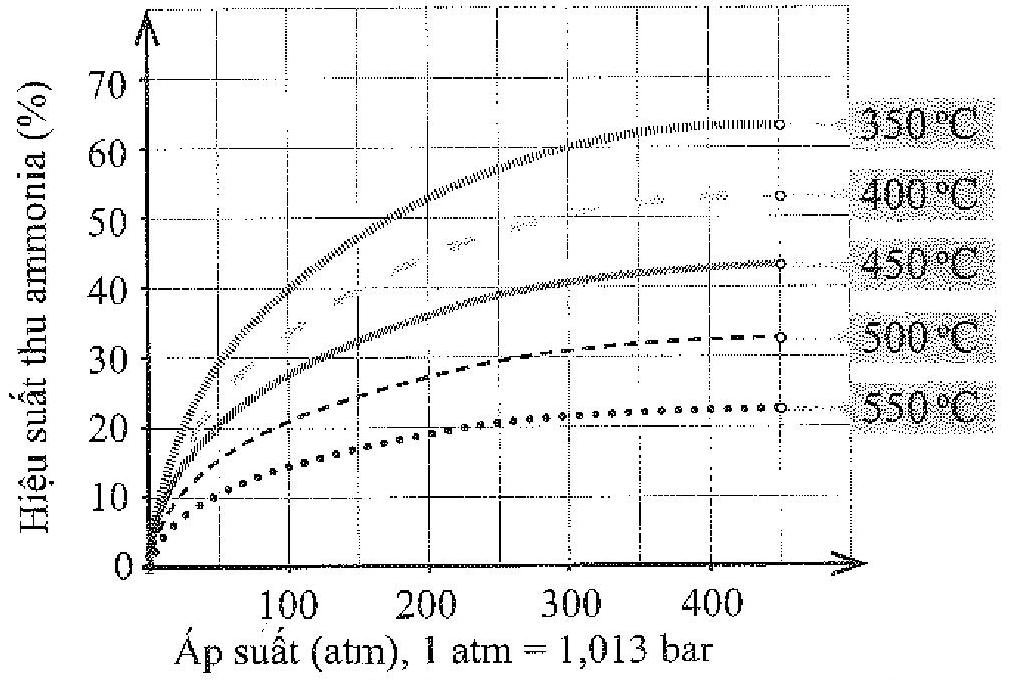
\includegraphics[width=\textwidth]{2025_10_23_f2823ef970776205e47bg-16}
\captionsetup{labelformat=empty}
\caption{Hình 5. Sụ phụ thuộc của hiệu suất tổng hợp ammonia vào áp suất và nhiệt độ phản ứng (Nguồn: Cowbridge Chemistry Department: Making ammonia - The Haber process http://ccschemistry.blogspot.com/2016/, truy câp ngày 22-3-2023.)}
\end{center}
\end{figure}

Hiệu suất thu ammonia có thể được tính theo công thức:

$$
\text { Hiệu suât }=\frac{\text { lượng } \mathrm{NH}_{3} \text { thu đươc trong thực tế }}{\text { lượng } \mathrm{NH}_{3} \text { tính theo li thuyết }} \times 100(\%)
$$

Khi phản ưng ưu tiên diễn ra theo chiều thuận thì lượng ammonia thu được trong thực tế càng nhiều.\\
a) Trong khoảng từ $350^{\circ} \mathrm{C}$ đến $550^{\circ} \mathrm{C}$, hiệu suất thu ammonia biến đổi theo xu hướng nào?\\
b) Vi sao nhiệt độ phản ứng càng cao thì hiệu suất thu ammonia càng thấp?\\
c) Ở một nhiệt độ, vì sao áp suất tăng cao thì hiệu suất thu ammonia tăng?\\
d) Từ giản đồ Hình 5, hãy cho biết nên chọn nhiệt độ phản ứng là bao nhiêu để hiệu suất phản ứng đạt khoảng $44 \%$ ở 200 atm .\\
5.5. Viết các phương trình hoá học của phản ứng sản xuất $\mathrm{NH}_{4} \mathrm{Cl}, \mathrm{NH}_{4} \mathrm{NO}_{3}$, $\left(\mathrm{NH}_{4}\right)_{2} \mathrm{SO}_{4}$ và $\left(\mathrm{NH}_{2}\right)_{2} \mathrm{CO}$ từ ammonia để làm phân bón vô co. Cho biết đó có phải là các phản ứng oxi hoá - khử không. Những phản ứng trên có tạo thành chất gây ô nhiễm môi trường không?\\
5.6. Giá trị biến thiên enthalpy chuẩn quá trình hoà tan trong nước của urea và ammonium sulfate lần lượt là $15,4 \mathrm{~kJ} \mathrm{~mol}^{-1}$ và $6,60 \mathrm{~kJ} \mathrm{~mol}^{-1}$.\\
a) Có hai ống nghiệm cùng dung tích. Mỗi ống nghiệm được đặt vừa khít vào lỗ trống đã được khoét sẵn trên miếng xốp cách nhiệt dày. Cho vào mỗi ống nghiệm 10 mL nước ở cùng nhiệt độ. Cắm nhiệt kế thuỷ ngân cùng loại vào mỗi ống nghiệm. Chờ dung dịch ổn định đến nhiệt độ phòng; sau đó, cho 2 gam phân bón urea vào ống nghiệm thứ nhất, 2 gam phân bón ammonium sulfate vào ống nghiệm thứ hai. Nhanh chóng dùng đũa thuỷ tinh khuấy nhẹ để phân bón tan hết. Mức thuỷ ngân trong nhiệt kế ở ống nghiệm nào sẽ thấp hơn? Giải thích.\\
b) Có thể phân biệt nhanh phân bón urea và phân bón ammonium sulfate bằng một lượng nước phù hợp được không? Giải thích.\\
5.7. Trong các công thức dưới đây, có bao nhiêu công thức không thoả mãn quy tắc octet?\\
$: \mathrm{N} \equiv \mathrm{N}:$\\
(1)\\
$\ddot{\mathrm{O}}=\mathrm{N}-\ddot{\mathrm{O}}$\\
(2)\\
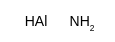
\includegraphics{smile-8e0175b473b9085073209b97a6c91ef4957e25e6}

(3)\\
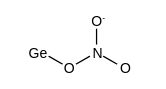
\includegraphics{smile-83155edbed62910f03cb988893df7ee3689e4167}

(4)\\
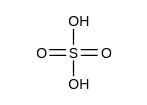
\includegraphics{smile-9fcf05af3e35e45f388cba59cf0161cabb37f389}

(5)\\
A. 1 .\\
B. 2 .\\
C. 3 .\\
D. 4 .\\
5.8. a) Viết cấu hình electron của nguyên tử nitrogen $(\mathrm{T})$ theo ô orbital. Nguyên tử N có bao nhiêu electron hoá trị ghép đôi, bao nhiêu electron hoá trị độc thân?\\
b) Có hai đề xuất về công thức Lewis của phân tự $\mathrm{HNO}_{3}$ như bên:\\
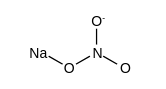
\includegraphics{smile-7a123878913c2d837f7c82071f77429838af884a}\\
(A)\\
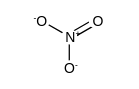
\includegraphics{smile-627b27d25b0f6ece64194fe4d9e46228335f3220}\\
(B)\\
b1) Công thức $(\mathrm{A})$ hay ( B ) phù hợp với đặc điểm các electron hoá trị của nguyên tữ nitrogen? Theo công thức đó, hoá trị và số oxi hoá của N là bao nhiêu?\\
$\mathrm{b} 2^{*}$ ) Kết quả nghiên cứu cho biết giá trị độ dài các liên kết giữa nguyên tử N và O (liên kết NO ) trong phân tử $\mathrm{HNO}_{3}$ là $1,406 \AA ; 1,211 \AA$ và $1,199 \AA$. Công thức (A) hay (B) có thể thoả mãn các số liệu đã cho? Giải thích.\\
5.9. Cho hai quá trình sau:

$$
\begin{array}{ll}
\mathrm{NH}_{4} \mathrm{NO}_{3}(s) \rightarrow \mathrm{N}_{2} \mathrm{O}(g)+2 \mathrm{H}_{2} \mathrm{O}(g) & \Delta_{\mathrm{r}} \mathrm{H}_{298}^{\circ}=-36 \mathrm{~kJ} \\
\mathrm{NH}_{4} \mathrm{Cl}(s) \rightarrow \mathrm{NH}_{3}(g)+\mathrm{HCl}(g) & \Delta_{\mathrm{r}} \mathrm{H}_{298}^{\circ}=176 \mathrm{~kJ}
\end{array}
$$

Ammonium nitrate và ammonium chloride được sử dụng làm phân bón. Trong quá trình lưu trữ, dưới ảnh hưởng của nhiệt, phân bón nào có nguy cơ cháy, nổ cao hơn? Giải thích.\\
5.10. Trong quy trình sản xuất tơ, mỗi năm có hàng triệu tấn cyclohexanone ( $\mathrm{C}_{6} \mathrm{H}_{10} \mathrm{O}$ ) được cho phản ứng với $\mathrm{HNO}_{3}$ để tạo adipic acid $\left(\mathrm{C}_{6} \mathrm{H}_{10} \mathrm{O}_{4}\right)$ theo phản ứng:

$$
\mathrm{C}_{6} \mathrm{H}_{10} \mathrm{O}+\mathrm{HNO}_{3} \rightarrow \mathrm{C}_{6} \mathrm{H}_{10} \mathrm{O}_{4}+\mathrm{N}_{2} \mathrm{O}+\mathrm{H}_{2} \mathrm{O}
$$

a) Cân bằng phương trình hoá học của phàn ứng trên theo phương pháp thăng bằng electron.\\
b) Cho biết vai trò của $\mathrm{HNO}_{3}$ trong phản ứng trên. Giải thích.\\
5.11. Vàng tan trong hỗn hợp gồm dung dịch nitric acid đặc và dung dịch hydrochloric acid đặc (tỉ lệ $1: 3$ về thể tích) tạo ra hợp chất tan của $\mathrm{Au}^{3+}$ theo phản ứng sau:

$$
\mathrm{Au}+\mathrm{HNO}_{3}+\mathrm{HCl} \rightarrow \mathrm{HAuCl}_{4}+\mathrm{H}_{2} \mathrm{O}+\mathrm{NO}
$$

a) Cân bằng phương trình hoá học của phản ứng trên theo phương pháp thăng bằng electron.\\
b) Cho biết acid nào đóng vai trò chất oxi hoá trong phản úng trên. Giải thích.

\section*{131}
\begin{enumerate}
  \setcounter{enumi}{5}
  \item SULFUR VÀ SULFUR DIOXIDE\\
6.1. Những phát biểu nào sau đây là đúng?\\
(a) Trong tự nhiên, sulfur tồn tại chủ yếu ở dạng muối sulfide và muối sulfate của một số kim loại.\\
(b) Là một phi kim khá hoạt động nên trong tự nhiên không tìm thấy sulfur đơn chất.\\
(c) Trứng gà ung có mùi thối đặc trưng một phần là do các hợp chất của sulfur có trong trứng phân huỷ gây ra.\\
(d) Nguyên tố sulfur có mặt trong một số loại thực vật, đặc biệt là các loại rau quả có mùi mạnh như hành tây, sầu riêng,...\\
(e) Thành phần chính của quặng pyrite là hợp chất của sulfur và chỉ (lead, Pb ).\\
6.2. Phân tử sulfur, $\mathrm{S}_{8}$, có cấu tạo như Hình 6 .\\
a) Giải thích vì sao phân tử này không phân cực.\\
b) Những phát biểu nào dưới đây là phù hợp với tính không phân cực của sulfur?\\
(b1) Hầu như không tan trong nước.\\
(b2) Tan nhiều trong dung môi ethanol.\\
(b3) Tan tốt trong dung môi không phân cực như carbon disulfide $\left(\mathrm{CS}_{2}\right)$.
\end{enumerate}

\begin{figure}[h]
\begin{center}
  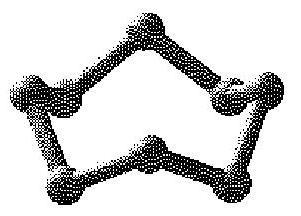
\includegraphics[width=\textwidth]{2025_10_23_f2823ef970776205e47bg-18}
\captionsetup{labelformat=empty}
\caption{Himin 6}
\end{center}
\end{figure}

(b4) Có tính sát khuần.\\
6.3. Thành phần chính của khí thiên nhiên là các hydrocarbon như methane (khoảng $80-85 \%$ ), ethane, propane, butane cùng lượng nhỏ các khí carbon dioxide, hydrogen sulfide, nitrogen. Thành phần chính cúa than là carbon, ngoài ra còn có một số hợp chất của các nguyên tố $\mathrm{H}, \mathrm{S}, \mathrm{O}, \mathrm{N}, \ldots$\\
Khi sử dụng khí thiên nhiên hoặc than làm nhiên liệu đều thải vào không khí các chất khí gây ô nhiễm. Giải thích.\\
6.4. Những ý kiến nào sau đây về sulfur dioxide ( $\mathrm{SO}_{2}$ ) là đúng?\\
(a) Có độc tính đối với con người.\\
(b) Phản ứng được với đá vôi.\\
(c) Khí này được tạo thành từ hoạt động của núi lửa trong tự nhiên, từ quá trình đốt cháy nhiên liệu hoá thạch của con người,...\\
(d) Là oxide lưỡng tính.\\
6.5. Nối những đặc điểm của chất ở cột B với tên chất ở cột A cho phù hợp.

\section*{Côt A}
a) Sulfur\\
b) Sulfur dioxide

\section*{Cột B}
\begin{enumerate}
  \item Là chất khí ở điều kiện thường.
  \item Ở điều kiện thường, phân tử có 8 nguyên tử.
  \item Dễ tan trong nước.
  \item Hoà tan trong dung môi phù hợp để làm thuốc trị bệnh ngoài da.
  \item Dừng để tẩy trắng vải, sợi.
  \item Có tính khữ và tính oxi hoá.\\
6.6. Trong phản ứng, $\mathrm{SO}_{2}$ có thể đóng vai trò là một oxide acid (acidic oxide). Hoàn thành các phương trình hoá học dưới đây để minh hoạ vai trò oxide acid cua $\mathrm{SO}_{2}$.\\
a) Tan trong nước tạo thành acid yếu $\mathrm{H}_{2} \mathrm{SO}_{3}$.\\
b) Phản ứng với dung dịch base tạo muối và nước.\\
c) Phản ứng với oxide base (basic oxide) tạo muối.\\
6.7. Cho giá trị enthalpy tạo thành chuẩn của khí $\mathrm{SO}_{2}$ và khí $\mathrm{SO}_{3}$ lần lượt là $-296,8 \mathrm{~kJ} \mathrm{~mol}^{-1}$ và $-395,7 \mathrm{~kJ} \mathrm{~mol}^{-1}$.\\
Tính giá trị biến thiên enthalpy chuẩn của phản ứng sau:
\end{enumerate}

$$
\mathrm{SO}_{2}(g)+\frac{1}{2} \mathrm{O}_{2}(g) \rightarrow \mathrm{SO}_{3}(g)
$$

Từ đó, hãy cho biết phản ứng trên có thuận lợi về mặt năng lượng không.\\
6.8. Một số quá trình tự nhiên và hoạt động của con ngừi thải hydrogen sulfide vào không khí. Chất này có thể bị oxi hoá bởi oxygen có trong không khí theo hai phản ứng sau:


\begin{align*}
& \mathrm{H}_{2} \mathrm{~S}(g)+\frac{3}{2} \mathrm{O}_{2}(g) \rightarrow \mathrm{SO}_{2}(g)+\mathrm{H}_{2} \mathrm{O}(g)  \tag{1}\\
& \mathrm{H}_{2} \mathrm{~S}(g)+\frac{1}{2} \mathrm{O}_{2}(g) \rightarrow \mathrm{S}(s)+\mathrm{H}_{2} \mathrm{O}(g) \tag{2}
\end{align*}


Cho biết giá trị enthalpy tạo thành chuẩn của $\mathrm{H}_{2} \mathrm{~S}(\mathrm{~g}), \mathrm{SO}_{2}(\mathrm{~g})$ và $\mathrm{H}_{2} \mathrm{O}(\mathrm{g})$ lần lượt là: $-20,7 \mathrm{~kJ} \mathrm{~mol}^{-1} ;-296,8 \mathrm{~kJ} \mathrm{~mol}^{-1}$ và $-241,8 \mathrm{~kJ} \mathrm{~mol}^{-1}$.\\
a) Tính giá trị biến thiên enthalpy chuẩn của mỗi phản ứng trên. Ở 298 K , mỗi phản ứng có thuận lợi về mặt năng lượng không?\\
b) Trong môi trường không khí mà nồng độ oxygen bị suy giảm, hãy dự đoán hydrogen sulfide sẽ dễ chuyển hoá thành sulfur dioxide hay sulfur. Giải thích.\\
6.9. Bột đá vôi có thể được sử dụng để xử lí khí thải chứa sulfur dioxide từ các nhà máy điện đốt than và dầu mỏ. Phương trình hoá học của phản ứng là:

$$
\mathrm{CaCO}_{3}(s)+\mathrm{SO}_{2}(g) \rightarrow \mathrm{CaSO}_{3}(s)+\mathrm{CO}_{2}(g)
$$

a) Vì sao phản ứng trên được gọi là phản ứng khử sulfur trong khí thải?\\
b) Tính giá trị biến thiên enthalpy chuẩn của phản ứng trên theo số liệu giá trị enthalpy tạo thành chuẩn của các hợp chất trong bảng sau đây. Cho biết phản ứng có thuận lợi về mặt năng lượng không.

\begin{center}
\begin{tabular}{|c|c|c|c|c|}
\hline
$H$ op chát & $\mathrm{CaSO}_{3}(s)$ & $\mathrm{CaCO}_{3}(s)$ & $\mathrm{SO}_{2}(g)$ & $\mathrm{CO}_{2}(g)$ \\
\hdashline
$\Lambda_{1} \mathrm{H}_{292}\left(\mathrm{k} / \mathrm{mol}^{-1}\right)$ & $-1634,9$ & $-1207,6$ & $-296,8$ & $-393,5$ \\
\hline
\end{tabular}
\end{center}

c) Trong phản ứng trên, vì sao đá vôi phải được dùng ở dạng bột?\\
d) Calcium sulfite ( $\mathrm{CaSO}_{3}$ ) thường được chuyển hoá thành thạch cao có công thức $\mathrm{CaSO}_{4} \cdot 2 \mathrm{H}_{2} \mathrm{O}$. Phản ứng hoá học chuyển $\mathrm{CaSO}_{3}$ thành $\mathrm{CaSO}_{4} \cdot 2 \mathrm{H}_{2} \mathrm{O}$ có thuộc loại phản ứng oxi hoá - khử không? Giải thích.

\section*{BAI \\
 7 SULFURIC ACID VÀ MUÓI SULFATE}
7.1. Những phát biểu nào sau đây là đúng?\\
(a) Sulfuric acid tan tốt trong nước, quá trình hoà tan toả nhiệt mạnh.\\
(b) Dung dịch sulfuric acid đặc hoà tan được tất cả các kim loại.\\
(c) Dung dịch sulfuric acid đặc có tính háo nước và tính oxi hoá mạnh.\\
(d) Dung dịch sulfuric acid loãng dễ bị phân huỷ bởi ánh sáng nên kém bền.\\
7.2. Những đặc điểm nào sau đây về muối sulfate là đúng?\\
(a) Nhiều muối sulfate tan tốt trong nước nhưng một số muối như $\mathrm{CaSO}_{4}$; $\mathrm{BaSO}_{4}$ rất ít tan trong nước.\\
(b) Magnesium sulfate được dùng làm thuốc điều trị bệnh liên quan đến hồng cầu, dùng làm chất hút mồ hôi tay cho các vận động viên,...\\
(c) Calcium sulfate là thành phần chính của các loại thạch cao. Phân tử chất này thường ngậm nước với số lượng các phân tử $\mathrm{H}_{2} \mathrm{O}$ khác nhau, tạo ra các loại thạch cao có ứng dụng khác nhau.\\
(d) Barium sulfate là chất rắn màu trắng, hầu như không tan trong nước. Chất này được dùng tạo màu trắng cho các loại giấy chất lượng cao.\\
7.3. Nối những đặc điểm của chất ở cột B với tên chất ở cột A cho phù hợp.

\section*{Côt A}
a) Sulfuric acid\\
b) Thạch cao\\
c) Ammonium sulfate (thành phần chính trong một loại phân đạm)

\section*{Côt B}
\begin{enumerate}
  \item Tan tốt trong nước.
  \item Là chất rắn ở điều kiện thường.
  \item Dừng để cố định xương bị gãy (bó bột).
  \item Là chất điện lì mạnh.
  \item Phản ứng dễ dàng với dung dịch base như nước vôi, barium hydroxide.
  \item Hoà tan được nhiều kim loại.\\
7.4. Hình bên là công thức Lewis của $\mathrm{H}_{2} \mathrm{SO}_{4}$.\\
a) Dựa vào công thức Lewis của $\mathrm{H}_{2} \mathrm{SO}_{4}$, hãy cho biết số oxi hoá của nguyên tử sulfur trong phân tử.\\
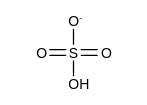
\includegraphics{smile-273326f278a4f10996755ca6a410142585b2caa5}\\
b) Khi tham gia phản ứng, $\mathrm{H}_{2} \mathrm{SO}_{4}$ không thể tạo ra các sản phẩm chứa sulfur có số oxi hoá lớn hơn hoặc bằng 7. Giải thích.\\
c) Hydrogen iodide có tính khử khá mạnh. Hãy dự đoán khí này có phản ứng với sulfuric acid đặc không. Giải thích.\\
7.5. Hãy mô tả hiện tượng xảy ra và hoàn thành phương trình hoá học của phản ứng xảy ra khi sulfuric acid loãng:\\
a) Tiếp xúc với lá kim loại hoạt động bị phủ bởi lớp oxide kim loại (chẳng hạn, lá kẽm (zinc) bị phủ bởi lớp zinc oxide).\\
b) Tiếp xúc với mẩu đá vôi hay mẩu phấn viết bảng.\\
c) Tiếp xúc bột baking soda (sodium hydrogencarbonate).\\
d) Được cho vào nước vôi trong, $\mathrm{Ca}(\mathrm{OH})_{2}$.\\
7.6. Dưới đây là một số phản ứng minh hoạ tính oxi hoá của sulfuric acid và sulfur dioxide. Đa số các phản ứng này có úng dụng trong phòng thí nghiệm. Hãy cân bằng phương trình hoá học các phản ứng bằng phương pháp thăng bằng electron.\\
a) Sulfuric acid đặc phản ứng với carbon trong than:
\end{enumerate}

$$
\mathrm{H}_{2} \mathrm{SO}_{4}(\text { đặc })+\mathrm{C} \rightarrow \mathrm{CO}_{2}+\mathrm{SO}_{2}+\mathrm{H}_{2} \mathrm{O}
$$

b) Sulfur dioxide làm mất màu dung dịch bromine:

$$
\mathrm{SO}_{2}+\mathrm{Br}_{2}+\mathrm{H}_{2} \mathrm{O} \rightarrow \mathrm{HBr}+\mathrm{H}_{2} \mathrm{SO}_{4}
$$

c) Sulfur dioxide làm mất màu dung dịch thuốc tím:

$$
\mathrm{SO}_{2}+\mathrm{KMnO}_{4}+\mathrm{H}_{2} \mathrm{O} \rightarrow \mathrm{MnSO}_{4}+\mathrm{K}_{2} \mathrm{SO}_{4}+\mathrm{H}_{2} \mathrm{SO}_{4}
$$

d) Sulfuric acid oxi hoá hợp chất $\mathrm{Fe}(\mathrm{II})$ thành hợp chất $\mathrm{Fe}(\mathrm{II})$ :

$$
\mathrm{H}_{2} \mathrm{SO}_{4}+\mathrm{FeSO}_{4} \rightarrow \mathrm{Fe}_{2}\left(\mathrm{SO}_{4}\right)_{3}+\mathrm{SO}_{2}+\mathrm{H}_{2} \mathrm{O}
$$

e) Phản ứng dùng để xác định nồng độ hợp chất Fe (II) bằng thuốc tím trong môi trường acid:

$$
\mathrm{H}_{2} \mathrm{SO}_{4}+\mathrm{FeSO}_{4}+\mathrm{KMnO}_{4} \rightarrow \mathrm{Fe}_{2}\left(\mathrm{SO}_{4}\right)_{3}+\mathrm{K}_{2} \mathrm{SO}_{4}+\mathrm{MnSO}_{4}+\mathrm{H}_{2} \mathrm{O}
$$

g) Phản ứng xác định nồng độ hợp chất $\mathrm{Fe}(\mathrm{II})$, dạng ion thu gọn:

$$
\mathrm{H}^{+}+\mathrm{Fe}^{2+}+\mathrm{MnO}_{4}^{-} \rightarrow \mathrm{Fe}^{3+}+\mathrm{Mn}^{2+}+\mathrm{H}_{2} \mathrm{O}
$$

7.7. Nhiều hộ gia đình thường trữ một số hoá chất như baking soda $\left(\mathrm{NaHCO}_{3}\right)$, thạch cao nung ( $\mathrm{CaSO}_{4} \cdot 0,5 \mathrm{H}_{2} \mathrm{O}$ ) và phèn chua (hay phèn nhôm kali, $\mathrm{K}_{2} \mathrm{SO}_{4} \cdot \mathrm{Al}_{2}\left(\mathrm{SO}_{4}\right)_{3} \cdot 24 \mathrm{H}_{2} \mathrm{O}$ hay $\left.\mathrm{KAl}\left(\mathrm{SO}_{4}\right)_{2} \cdot 12 \mathrm{H}_{2} \mathrm{O}\right)$.\\
a) Hãy tìm hiểu các ứng dụng của mỗi hoá chất trên tại các hộ gia đình.\\
b) Có thể dùng nước để phân biệt các mẫu bột mịn của ba chất trên không? Giải thích.\\
c) Có thể dùng nước và quỳ tím để phân biệt các mẫu bột mịn của ba chất trên không? Giải thích.\\
7.8. Sulfuric acid là một trong những hoá chất quan trọng nhất được sử dụng trong công nghiệp; được sản xuất hàng trăm triệu tấn mỗi năm, chiếm nhiều nhất trong ngành công nghiệp hoá chất. Phương pháp sản xuất sulfuric acid phổ biến nhất là phương pháp tiếp xúc, theo đó acid có thể được điều chế qua các giai đoạn sau:

$$
\begin{aligned}
& \text { (1) } \mathrm{FeS}_{2}(s)+\mathrm{O}_{2}(g) \stackrel{\mathrm{t}^{\circ}}{\leftrightarrows} \mathrm{Fe}_{2} \mathrm{O}_{3}(s)+\mathrm{SO}_{2}(g) \\
& \text { (2) } \mathrm{SO}_{2}(g)+\mathrm{O}_{2}(g) \stackrel{450^{\circ} \mathrm{C}, \mathrm{~V}_{2} \mathrm{O}_{5}}{=} \mathrm{SO}_{3}(g) \quad \Delta_{\mathrm{r}} \mathrm{H}_{298}^{\circ}=-196 \mathrm{~kJ}
\end{aligned}
$$

(3) $\mathrm{H}_{2} \mathrm{SO}_{4}(a q)+\mathrm{SO}_{3}(g) \rightarrow \mathrm{H}_{2} \mathrm{SO}_{4} \cdot \mathrm{nSO}_{3}(l)$\\
(4) $\mathrm{H}_{2} \mathrm{SO}_{4} \cdot \mathrm{nSO}_{3}(l)+\mathrm{H}_{2} \mathrm{O}(l) \rightarrow \mathrm{H}_{2} \mathrm{SO}_{4}(a q)$\\
a) Cân bằng phương trình hoá học của các phản ứng trên.\\
b) Theo nguyên lí chuyển dịch cân bằng, phản ứng (2) nên được thực hiện ở nhiệt độ cao hay thấp? Trong thực tế, phản ứng trên được thực hiện ở nhiệt độ khá cao ( $450^{\circ} \mathrm{C}$ ), hãy giải thích điều này.\\
c) Người ta dùng sulfuric acid đặc $\mathrm{H}_{2} \mathrm{SO}_{4}(a q)$ hấp thụ $\mathrm{SO}_{3}(g)$ trong phản ứng ( 3 ), quá trình này được thực hiện trong tháp tiếp xúc. Cách thực hiện nào sau đây sẽ đạt hiệu quả tiếp xúc tốt nhất?\\
A. Cho $\mathrm{SO}_{3}(g)$ lội qua dung dịch $\mathrm{H}_{2} \mathrm{SO}_{4}(a q)$.\\
B. $\mathrm{SO}_{3}(g)$ được phun vào từ phía trên tháp, $\mathrm{H}_{2} \mathrm{SO}_{4}(a q)$ được bơn từ dưới lên.\\
C. $\mathrm{SO}_{3}(g)$ được xả vào từ phía dưới tháp, $\mathrm{H}_{2} \mathrm{SO}_{4}(a q)$ được phun từ trên xuống.\\
D. $\mathrm{SO}_{3}(\mathrm{~g})$ lội qua $\mathrm{H}_{2} \mathrm{SO}_{4}(\mathrm{aq})$ được khuấy liên tục với tốc độ cao.\\
d) Để xác định công thức của oleum thu được, người ta pha loãng $8,36 \mathrm{gam}$ oleum vào nước thành 1,0 lít dung dịch sulfuric acid, sau đó tiến hành chuẩn độ mỗi $10,0 \mathrm{~mL}$ dung dịch acid này bằng dung dịch $\mathrm{NaOH} 0,10 \mathrm{M}$. Thể tích NaOH trung bình cần sử dụng để chuẩn độ là $20,01 \mathrm{~mL}$. Hãy xác định công thức của oleum trên.\\
7.9. Trong công nghiệp, chất rắn copper(II) sulfate pentahydrate có thể được sản xuất từ copper(II) oxide theo hai giai đoạn của quá trình:

$$
\mathrm{CuO}(s) \xrightarrow{\text { dung dịch } \mathrm{H}_{2} \mathrm{SO}_{4} \text { loâng }} \mathrm{CuSO}_{4}(a q) \xrightarrow{\text { kêt timh }} \mathrm{CuSO}_{4} \cdot 5 \mathrm{H}_{2} \mathrm{O}(s)
$$

a) Từ 1 tấn nguyên liệu chứa $96 \%$ copper(II) oxide theo khối lượng (còn lại là tạp chất tro) sẽ thu được bao nhiêu kilògam copper(II) sulfate pentahydrate rắn? Cho hiệu suất của quá trình là $85 \%$.\\
b) Một ao nuôi thuỷ sản có diện tích bề mặt nước là $2000 \mathrm{~m}^{2}$, độ sâu trung bình của nước trong ao là $0,7 \mathrm{~m}$ đang có hiện tượng phú đương. Để xử lí tảo xanh có trong ao, người dân cho copper(II) sulfate pentahydrate vào ao trong 3 ngày, mỗi ngày một lần, mỗi lần là $0,25 \mathrm{~g}$ cho $1 \mathrm{~m}^{3}$ nước trong ao. Hãy cho biết tổng khối lượng (kg) copper(II) sulfate pentahydrate người dân cần sử dụng.\\
c) Có thể pha chế dung dịch copper(II) sulfate $10^{-4} \mathrm{M}$ dùng để diệt một số loai vi sinh vật. Tính số mg copper(II) sulfate pentahydrate cần dùng để pha chế thành 1 L dung dịch copper(II) sulfate $10^{-4} \mathrm{M}$.

\section*{CHỦ ĐỀ 3 DAI CƯONG VỂ HOÁ HOC HƯU CÓ}
BKI 8 HỢP CHẤT HỰU CO VÀ HOÁ HOC HÜU CƠ\\
8.1. Những phát biểu nào sau đây là đúng?\\
(a) Nguyên tố carbon và hydrogen luôn có mặt trong thành phần hợp chất hữu cơ.\\
(b) Họp chất hữu cơ mà thành phần phân tử chỉ gồm các nguyên tố carbon và hydrogen là hydrocarbon.\\
(c) Hợp chất hữu co là hợp chất của carbon (trừ $\mathrm{CO}, \mathrm{CO}_{2}$, các muối carbonate, các hợp chất cyanide, các carbide,...).\\
(d) Phổ hồng ngoại cho phép xác định cả loại nhóm chức và số lượng nhóm chức đó có trong phân tử hữu cơ.\\
(e) Phổ hồng ngoại cho phép xác định loại nhóm chức có trong phân tử hữu cơ.\\
(g) Một hydrocarbon và một hợp chất ion có khối lượng phân tử gần bằng nhau thì hydrocarbon tan trong nước ít hơn và có nhiệt độ sôi thấp hơn so với hợp chất ion.\\
8.2. Chất nào dưới đây không là chất hữu cơ?\\
A. Acetic acid.\\
B. Urea.\\
C. Ammonium cyanate.\\
D. Ethanol.\\
8.3. Trường hợp nào dưới đây khoanh đúng nhóm chức carboxylic acid của ethanoic acid?

A.\\
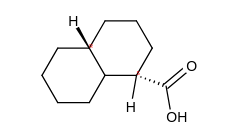
\includegraphics{smile-dbddce577a3a9209a6e82441554e0d606d13ce0d}

B.\\
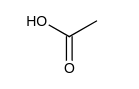
\includegraphics{smile-cff4f83455b57b615286ec7f92504766c01a0d70}

C.\\
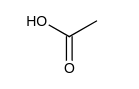
\includegraphics{smile-9bd4e7b92314042ae9e413bf212464ce052593a7}

D.\\
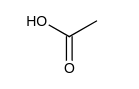
\includegraphics{smile-6acec17f1436fbba09816c88b9d86f07d6dc18d9}\\
8.4. Trên phổ hồng ngoại của hợp chất hữu cơ X có các hấp thụ đặc trưng ở $2817 \mathrm{~cm}^{-1}$ và $1731 \mathrm{~cm}^{-1}$. Chất X là chất nào trong các chất dưới đây?\\
A. $\mathrm{CH}_{3} \mathrm{C}(\mathrm{O}) \mathrm{CH}_{2} \mathrm{CH}_{3}$.\\
B. $\mathrm{CH}_{2}=\mathrm{CHCH}_{2} \mathrm{CH}_{2} \mathrm{OH}$.\\
C. $\mathrm{CH}_{3} \mathrm{CH}_{2} \mathrm{CH}_{2} \mathrm{CHO}$.\\
D. $\mathrm{CH}_{3} \mathrm{CH}=\mathrm{CHCH}_{2} \mathrm{OH}$.\\
8.5. Phổ hồng ngoại của họp chất hữu cơ nào dưới đây không có hấp thụ ở vùng $1750-1600 \mathrm{~cm}^{-1}$ ?\\
A. Alcohol.\\
B. Ketone.\\
C. Ester.\\
D. Aldehyde.\\
8.6. Vì sao có thể dựa vào nhóm chức để phân loại các hợp chất hữu cơ?\\
A. Vi biết được nhóm chức thì biết được thành phần các nguyên tố hoá học có trong phân tử hợp chất hữu co.\\
B. Vì nhóm chức không bị biến đổi khi phân tử hữu cơ tham gia phản ứng.\\
C. Vì nhóm chức tham gia vào các phản ứng trong cơ thể sống.\\
D. Vì nhóm chức gây ra các phản ứng hoá học đặc trưng cho phân tử hũu co.\\
8.7. Phân tử của mỗi chất $\mathrm{A}, \mathrm{B}$ và D chứa một trong các nhóm chức: alcohol, ketone hoặc carboxylic acid. Biết rằng trên phổ $\mathrm{IR}, \mathrm{A}$ cho các hấp thụ đặc trưng ở $2690 \mathrm{~cm}^{-1}$ và $1715 \mathrm{~cm}^{-1}$; B chỉ có hấp thụ đặc trưng ở $3348 \mathrm{~cm}^{-1}$ còn D cho hấp thụ đặc trưng ở $1740 \mathrm{~cm}^{-1}$. Cho biết nhóm chức có trong phân tữ mỗi chất $\mathrm{A}, \mathrm{B}$ và D .\\
8.8. Cho dãy chuyển hoá sau:

$$
\mathrm{CaO} \xrightarrow{(1)} \mathrm{CaC}_{2} \xrightarrow{(2)} \mathrm{C}_{2} \mathrm{H}_{2} \xrightarrow{(3)} \mathrm{CH}_{3} \mathrm{CHO}
$$

calcium oxide calcium carbide acetylene acetaldehyde\\
Trong các chuyển hoá trên, chuyển hoá nào được thực hiện bằng phản ứng hoá học:\\
a) giữa hai chất vô cơ?\\
b) giữa hai chất hữu cơ?\\
c) giữa chất vô cơ và chất hữu cơ?\\
8.9. Thực hiện thí nghiệm đốt cháy hỗn hợp alkane lỏng (C10 - C15) như mô tả trong Hinh 8.1.\\
a) Chất lỏng không màu trong ống chữ U là chất gì? Cho biết vai trò của nước

\begin{figure}[h]
\begin{center}
  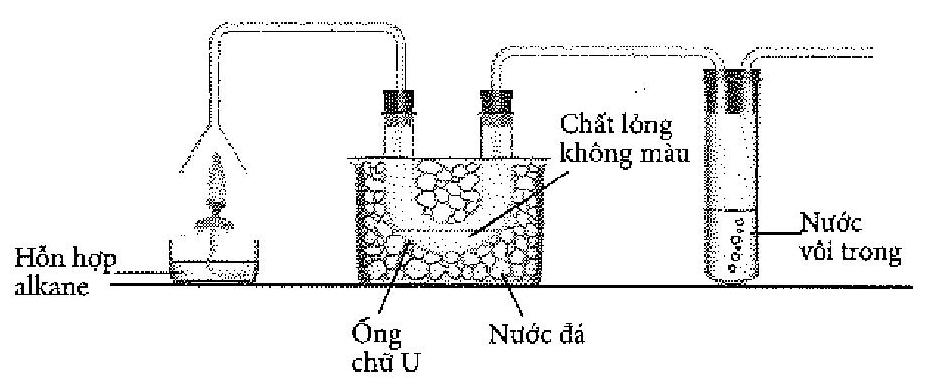
\includegraphics[width=\textwidth]{2025_10_23_f2823ef970776205e47bg-25}
\captionsetup{labelformat=empty}
\caption{Hinh 8.1}
\end{center}
\end{figure}

đá trong thí nghiệm trên.\\
b) Vì sao sau khi đốt alkane một thời gian thì thấy nước vôi trong vẩn đục?\\
c) Thí nghiệm này chứng tỏ những nguyên tố nào có mặt trong alkane?\\
8.10. Đốt cháy hoàn toàn chất A tạo thành $\mathrm{CO}_{2}$ và $\mathrm{H}_{2} \mathrm{O}$.\\
a) Trình bày phương pháp nhận ra sự có mặt của $\mathrm{CO}_{2}$ và $\mathrm{H}_{2} \mathrm{O}$ trong sản phẩm cháy.\\
b) Những nguyên tố nào chắc chắn có mặt trong chất A ? Nguyên tố nào có thể có trong thành phần chất A ? Cần thêm dữ kiện nào để chắc chắn điều này?\\
c) Trên phổ IR của $\mathbf{A}$ thấy có hấp thụ ở $1720 \mathrm{~cm}^{-1}$. Nhóm chức nào có thể có trong phân tử chất A ?\\
8.11. Phổ IR của chất A được cho như Hinh 8.2.

A có thể là chất nào trong số các chất sau: (1) $\mathrm{CH}_{3} \mathrm{CH}_{2}-\mathrm{COOH}$,\\
(2) $\mathrm{CH}_{3} \mathrm{CH}_{2} \mathrm{CH}_{2}-\mathrm{CHO}$,\\
(3) $\mathrm{CH}_{3} \mathrm{CH}_{2}-\mathrm{NH}-\mathrm{CH}_{2} \mathrm{CH}_{3}$ và\\
(4) $\mathrm{CH}_{3} \mathrm{COCH}_{2} \mathrm{CH}_{3}$ ? Giải thích.

\begin{figure}[h]
\begin{center}
  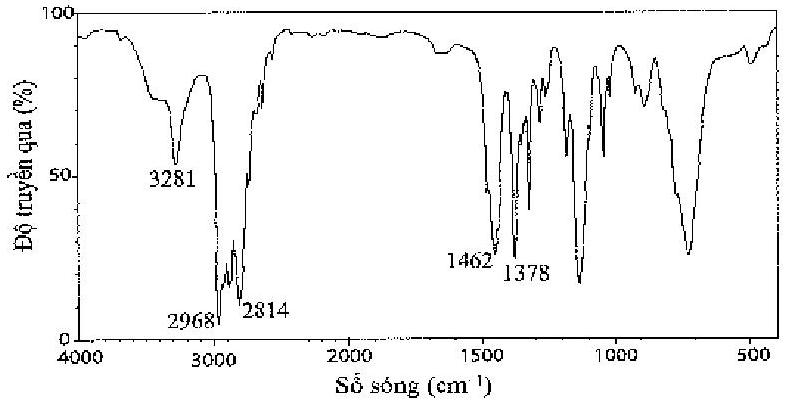
\includegraphics[width=\textwidth]{2025_10_23_f2823ef970776205e47bg-26(1)}
\captionsetup{labelformat=empty}
\caption{Hinh 8.2}
\end{center}
\end{figure}

8.12. Cho các chất formic acid, acetic acid và methyl formate như sau:\\
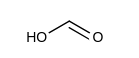
\includegraphics{smile-2aa327f244c1662e2030456916cea4258aa5ab28}

formic acid\\
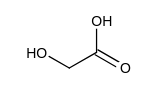
\includegraphics{smile-bf9b9b09ab11bd5b2037ea7732a857470cf09070}

acetic acid\\
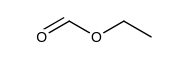
\includegraphics{smile-86eb5a2ef6166ef155757de0821cb72a048d9649}

methyl formate\\
a) Khoanh vào nhóm nguyên tử tạo thành nhóm chức acid hoặc nhóm chức ester có trong phân tử các chất trên.\\
b) Giải thích vì sao formic acid và methyl formate có thể thể hiện được tính chất hoá học đặc trưng của nhóm chức aldehyde.

\section*{BT. PHUONG PHÁP TÁCH BIẸT VA TINH CHÉ HOP CHÁT HÜU CO}
9.1. Một học sinh tiến hành chưng cất để tách $\mathrm{CHCl}_{3}\left(\mathrm{t}_{\mathrm{s}}=61^{\circ} \mathrm{C}\right)$ ra khòi $\mathrm{CHCl}_{2} \mathrm{CHCl}_{2}$ ( $\mathrm{t}_{\mathrm{s}}=146^{\circ} \mathrm{C}$ ) bằng bộ dụng cụ như ở Hình 9.1. Khi bắt đầu thu nhận $\mathrm{CHCl}_{3}$ vào bình húng thì nhiệt độ tại vị trí nào trong hình đang là $61^{\circ} \mathrm{C}$ ?\\
A. Vịtrí X .\\
B. VịtríY.\\
C. Vịtrí $Z$.\\
D. Vị trí T.

\begin{figure}[h]
\begin{center}
  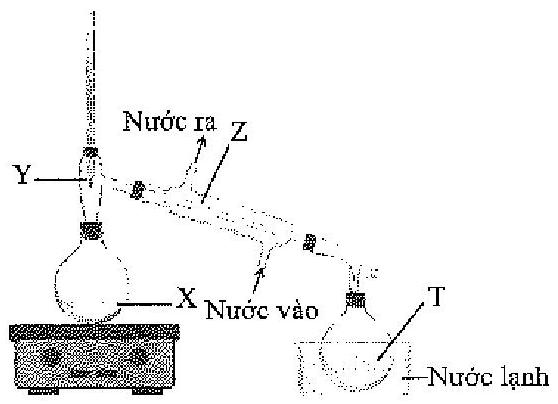
\includegraphics[width=\textwidth]{2025_10_23_f2823ef970776205e47bg-26}
\captionsetup{labelformat=empty}
\caption{Hinh 9.1}
\end{center}
\end{figure}

9.2. Hỗn hợ X gồm các alkane: pentane ( $\mathrm{t}_{\mathrm{s}}=36,1^{\circ} \mathrm{C}$ ), heptane ( $\mathrm{t}_{\mathrm{s}}=98,4^{\circ} \mathrm{C}$ ), octane ( $\mathrm{t}_{\mathrm{s}}=125,7^{\circ} \mathrm{C}$ ) và nonane ( $\mathrm{t}_{\mathrm{s}}=150,8^{\circ} \mathrm{C}$ ). Có thể tách riêng các chất đó một cách thuận lợi bằng phương pháp nào sau đây?\\
A. Kết tinh.\\
B. Chưng cất.\\
C. Sắc kí.\\
D. Chiết.\\
9.3. Tính chất vật lí nào sau đây được quan tâm khi tách hai chất lỏng tan vào nhau bằng phương pháp chưng cất?\\
A. Nhiệt độ sôi của chất.\\
B. Nhiệt độ nóng chảy của chất.\\
C. Tính tan của chất trong nước.\\
D. Mầu sắc của chất.\\
9.4. Việc tách các chất ra khỏi nhau bằng phương pháp sắc kí dựa trên đặc tính nào sau đây của chất?\\
A. Phân từ khối.\\
B. Nhiệt độ sôi.\\
C. Khả năng hấp phụ và hoà tan.\\
D. Nhiệt độ nóng chảy.\\
9.5. Sử dụng phương pháp kết tinh lại để tinh chế chất rẳn. Hợp chất cần kết tinh lại cần có tính chất nào dưới đây để việc kết tinh lại được thuận lợi?\\
A. Tan trong dung môi phân cực, không tan trong dung môi không phân cực.\\
B. Tan tốt trong cả dung dịch nóng và lạnh.\\
C. Ít tan trong cả dung dịch nóng và lạnh.\\
D. Tan tốt trong dung dịch nóng, ít tan trong dung dịch lạnh.\\
9.6. Ngâm củ nghệ với ethanol nóng, sau đó lọc bỏ phần bã, lấy đung dịch đem cô để làm bay hơi bớt dung môi. Phần dung dịch còn lại sau khi cô được làm lạnh, để yên một thời gian rồi lọc lấy kết tủa curcumin màu vàng. Từ mô tả ở trên, hãy cho biết, người ta đã sử dụng các kĩ thuật tinh chế nào để lấy được curcumin từ củ nghệ.\\
A. Chiết, chưng cất và kết tinh.\\
B. Chiết và kết tinh.\\
C. Chưng chất và kết tinh.\\
D. Chưng cất, kết tinh và sắc kí.\\
9.7. Pent-1-ene và dipentyl ether đồng thời được sinh ra khi đun nóng pentan-1-ol với dung dịch $\mathrm{H}_{2} \mathrm{SO}_{4}$ đặc. Biết rằng nhiệt độ sôi của pentan-1-ol, pent-1-ene và dipentyl ether lần lượt là $137,8^{\circ} \mathrm{C}, 30,0^{\circ} \mathrm{C}$ và $186,8^{\circ} \mathrm{C}$. Từ hỗn hợp phản ứng, các chất được tách khỏi nhau bằng phương pháp chưng cất. Các phân đoạn thu được (theo thứ tự từ trước đến sau) trong quá trình chưng cất lần lượt là\\
A. pentan-1-ol, pent-1-ene và dipentyl ether.\\
B. pent-1-ene, pentan-1-ol và dipentyl ether.\\
C. dipentyl ether, pent-1-ene và pentan-1-ol.\\
D. pent-1-ene, dipentyl ether và pentan-1-ol.\\
9.8. Vì sao phải cô lập và tinh chế các hợp chất hoá học? Kể tên một số phương pháp được dùng tinh chế chất hữu cơ mà em biết. Tìm hiểu và nêu ví dụ minh hoạ về việc áp dụng các phương pháp này để tinh chế chất hoá học trong đời sống.\\
9.9. Thêm hexane (một hydrocarbon trong phân tử có 6 nguyên tử carbon) vào dung dịch iodine trong nước, lắc đều rồi để yên. Sau đó thu lấy lớp hữu cơ, làm bay hoi dung môi để thu lấy iodine.\\
a) Phương pháp nào đã được sử dụng để thu lấy iodine từ dung dịch iodine trong nước trong quy trình được mô tả ở trên?\\
b) Hình 9.2 mô tả hiện tượng xảy ra trong dụng cụ dùng thu lấy iodine trong thí nghiệm trên. Cho biết tên của dụng cụ này.\\
c) Mô tả cách làm để tách riêng phần nước và phần hữu cơ từ dụng cụ ở Hình 9.2.\\
d) Giải thích sự khác nhau về màu sắc của lớp nước và lớp hữu cơ trong dụng cụ trên trước và sau khi lắc.

\begin{figure}[h]
\begin{center}
  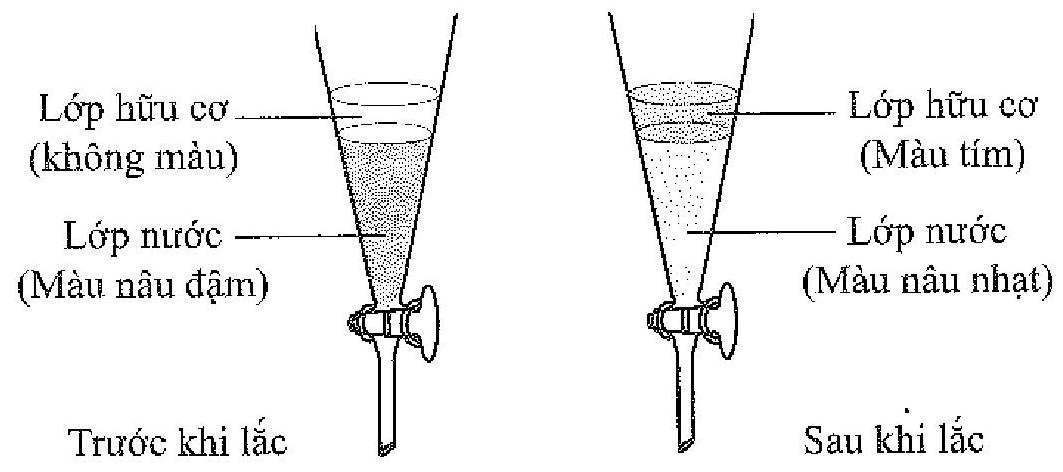
\includegraphics[width=\textwidth]{2025_10_23_f2823ef970776205e47bg-28(1)}
\captionsetup{labelformat=empty}
\caption{Hinh 9.2}
\end{center}
\end{figure}

9.10. Để tinh chế chất hữu cơ rắn chứa tạp chất, người ta hoà tan chất rắn trong dung môi thích họp rồi lọc bó tạp chất không $\tan$ (Hinh 9.3).\\
a) Đưa các chú thích trên hình (đã cho trong khung) vào các vị trí (A, B, C, D, E, F) cho phù hợ.

\begin{figure}[h]
\begin{center}
  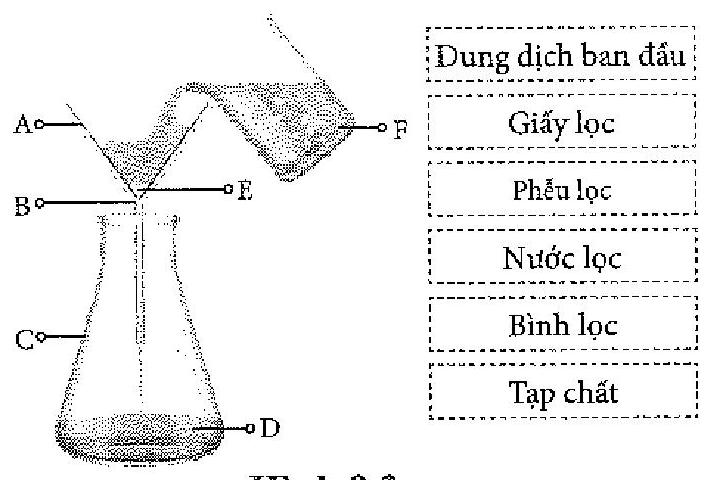
\includegraphics[width=\textwidth]{2025_10_23_f2823ef970776205e47bg-28}
\captionsetup{labelformat=empty}
\caption{Hinih 9.3}
\end{center}
\end{figure}

b) Để yên nước lọc một thời gian nhưng chưa thấy chất rắn kết tinh như mong muốn. Yếu tố nào có thể là nguyên nhân của hiện tượng này?\\
c) Cần làm gì để có thể có được chất rắn kết tinh từ đung dịch thu được ở trường họp b ).\\
d) Cho biết tên của phương pháp đã sử dụng để tinh chế chất rắn ở trên.\\
9.11. Một học sinh tiến hành kết tinh lại để tinh chế một chất hữu cơ rắn có nhiễm chất bẩn và vẽ lại quá trình tiến hành như ở Hình 9.4.\\
a) Mô tả quá trình kết tinh lại mà học sinh trên đã thực hiện.\\
b) Giải thích vì sao sau khi kết tinh lại thì chất rắn ban đầu lại sạch hon.\\
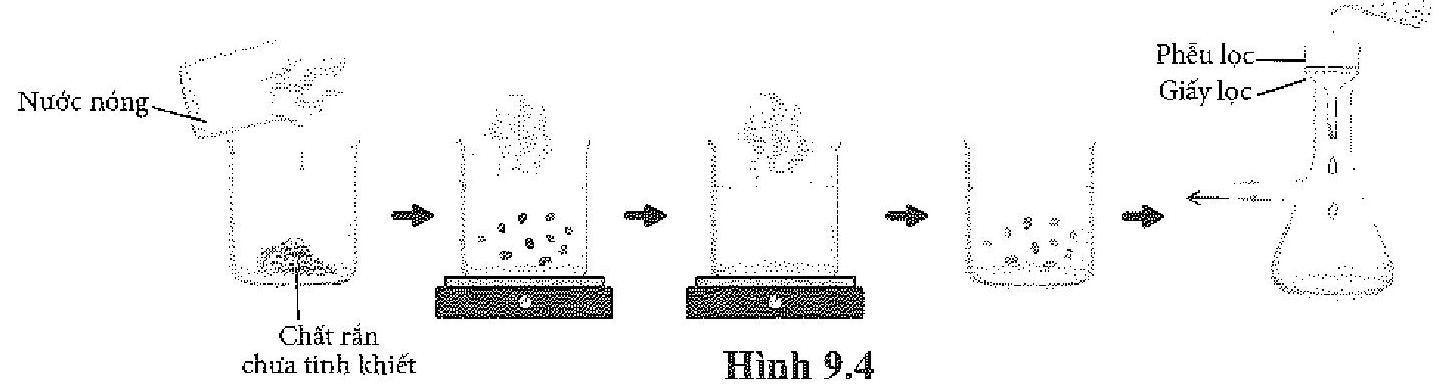
\includegraphics[max width=\textwidth, center]{2025_10_23_f2823ef970776205e47bg-29}\\
9.12. Benzene thương mại $\left(\mathrm{t}_{\mathrm{s}}=80,1^{\circ} \mathrm{C}\right)$ thu được từ quá trình chưng cất nhựa than đá chứa $3-5 \%$ thiophene ( $\mathrm{t}_{\mathrm{s}}=84,2^{\circ} \mathrm{C}$ ). Thiophene dược loại khỏi benzene bằng cách chiết với dung dịch sulfuric acid đậm đặc. Quá trình tinh chế này dựa trên co sở là phản ứng giữa sulfuric acid với thiophene xảy ra dễ dàng hơn nhiều so với benzene. Khi lắc benzene thưong mại với dung dịch sulfuric acid đậm đặc, chi thiophene phản ứng với sulfuric acid để tạo thành thiophene-2-sulfonic acid tan trong sulfuric acid. Chiết lấy lóp benzene, rưa nhiều lần bằng nước rồi làm khô bằng $\mathrm{CuSO}_{4}$ khan và đem chưng cất thu lấy benzene tinh khiết.\\
a) Benzene thương mại lẫn tạp chất gì? Vì sao không tiến hành chưng cất ngay benzene thưong mại để thu lấy benzene tinh khiết?\\
b) Ví sao sau khi xử lí benzene thương mại với dung dịch sulfuric acid đậm đặc thì loại bỏ được tạp chât?\\
c) Vì sao sau khi xử lí benzene thương mại với dung dịch sulfuric acid đậm đặc lại phải rưa benzene nhiều lần với nước?\\
d) Nước lẫn trong benzene được loại bó bằng cách nào? Dự đoán hiện tượng xây ra và cho biết làm sao để biết nước đã không còn trong benzene sau khi được xử lí.\\
9.13. Một mẫu hoa hoè được xác định có hàm lượng rutin là $26 \%$. Người ta đun sôi hoa hoè với nược ( $100^{\circ} \mathrm{C}$ ) để chiết lấy rutin. Biết độ tân của rutin là 5,2 gam trong 1 lít nước ở $100^{\circ} \mathrm{C}$ và là 0,125 gam trong 1 lít nước ở $25^{\circ} \mathrm{C}$.\\
a) Cần dùng thể tích nước tối thiểu là bao nhiêu để chiết được lượng rutin có trong 100 gam hoa hoè?\\
b) Giả thiết rằng toàn bộ lượng rutin trong hoa hoè đã tan vào nước khi chiết. Làm nguội dung dịch chiết 100 gam hoa hoè ở trên từ $100^{\circ} \mathrm{C}$ xuống $25^{\circ} \mathrm{C}$ thì thu được bao nhiêu gam rutin kết tinh?\\
c) Vì sao khi sử dụng lượng nước lớn hơn thì khối lượng rutin thu được khi kết tinh lại giảm đi?\\
9.14. Chuẩn bị các khuôn gỗ có kích thước $58 \mathrm{~cm} \times 80 \mathrm{~cm} \times 5 \mathrm{~cm}$, ở giữa có đặt tấm thuỷ tinh được quét mỡ lợn cả hai mặt, mỗi lớp dày 3 mm . Đặt lên trên bề mặt chất béo một lớp lụa mỏng rồi rải lên trên $30-80 \mathrm{~g}$ hoa tươi khô ráo, không bị dập nát. Khoảng 30-40 khuôn gỗ được xếp chồng lên nhau rồi để trong phòng kín. Sau khoảng $24-72$ giờ (tuỳ từng loại hoa), người ta thay lớp hoa mới cho đến khi lớp chất béo bão hoà tinh dầu.\\
a) Từ thông tin trên, hãy cho biết người ta đã sử dụng phương pháp nào để lấy tinh dầu từ hoa.\\
b) Cho biết vai trò của chất béo (mỡ lọn) trong quy trình thực hiện ở trên.\\
c) Đề xuất một phương pháp khác để lấy được tinh dầu hoa.

\section*{\textbackslash section*\{BAI\} \\
 10 CÔNG THƯC PHÂN TỦ HỢP CHÁT HƯU CƠ}
10.1. CFC (chlorofluorocarbon) là kí hiệu chung chỉ nhóm các hợp chất hữu cơ mà trong phân tứ có chưa ba loại nguyên tố $\mathrm{Cl}, \mathrm{F}$ và C . Uu điểm của chúng là rất bền, không cháy, không mùi, không độc, không gây ra sự ăn mòn, dễ bay hơi,... nên được dùng làm chất sinh hàn trong tủ lạnh, điều hoà không khí, dùng trong các bình xịt để tạo bọt xốp,....\\
Tuy nhiên, do có nhược điểm lớn là phá huỷ tầng ozone bảo vệ Trái Dất nên ừ những năm $1990, \mathrm{CFC}$ bị hạn chế sử dụng theo các quy định của các công ước về bảo vệ môi trường và chống biến đổi khí hậu:\\
Freon-12 là một loại chất CFC được sứ dụng khá phổ biến, có chứa $31,40 \%$ fluorine và $58,68 \%$ chlorine về khối lượng. Công thức phân tử của freon- 12 là\\
A. $\mathrm{CCl}_{3} \mathrm{~F}$.\\
B. $\mathrm{CCl}_{2} \mathrm{~F}_{2}$.\\
C. $\mathrm{CClF}_{3}$.\\
D. $\mathrm{C}_{2} \mathrm{Cl}_{4} \mathrm{~F}_{2}$.\\
10.2. Glyoxal có thành phần phần trăm khối lượng các nguyên tố là: $41,4 \% \mathrm{C}$; $3,4 \% \mathrm{H}$ và $55,2 \% \mathrm{O}$. Công thức nào dưới đây phù hợp với công thức thực nghiệm của glyoxal?\\
A. CHO .\\
B. $\mathrm{CH}_{2} \mathrm{O}$.\\
C. $\mathrm{CH}_{2} \mathrm{O}_{2}$.\\
D. $\mathrm{C}_{2} \mathrm{H}_{6} \mathrm{O}$.\\
10.3. Phát biểu nào sau đây là đúng?\\
A. Công thức thực nghiệm của chất có thể được xác định theo thành phần phần trăm về khối lượng của các nguyên tố có trong phân tử chất đó.\\
B. Công thức thực nghiệm của chất có thể được xác định qua phổ hồng ngoại của chất đó.\\
C. Công thức thực nghiệm của chất có thể được xác định qua phổ khối lượng của chất đó.\\
D. Công thức thực nghiệm của chất có thể được xác định qua các phản ứng hoá học đặc trưng của chất đó.\\
10.4. Phát biểu nào sau đây là không đúng?\\
A. Hai chất có cùng công thức thực nghiệm có thể có phân tử khối khác nhau.\\
B. Hai chất có cùng công thức thực nghiệm có phần trăm khối lượng các nguyên tố trong phân tử của chứng như nhau.\\
C. Hai chất có cùng công thức thực nghiệm thì thành phần các nguyên tố trong phân tử của chứng giống nhau.\\
D. Hai chất có cùng công thức thực nghiệm luôn có cùng công thức phân tư.\\
10.5. Phổ MS của chất Y cho thấy Y có phân tử khối bằng 60 . Công thức phân tữ nào dưới đây không phù hợp với Y ?\\
A. $\mathrm{C}_{3} \mathrm{H}_{8} \mathrm{O}$.\\
B. $\mathrm{C}_{2} \mathrm{H}_{4} \mathrm{O}_{2}$.\\
C. $\mathrm{C}_{3} \mathrm{H}_{7} \mathrm{~F}$.\\
D. $\mathrm{C}_{2} \mathrm{H}_{8} \mathrm{~N}_{2}$.\\
10.6. Acetic acid có công thức phân tử là $\mathrm{C}_{2} \mathrm{H}_{4} \mathrm{O}_{2}$. Kết luận nào dưới đây là đúng?\\
A. Acetic acid có công thức thực nghiệm là $\mathrm{CH}_{2} \mathrm{O}$ và có khối lượng riêng lớn gấp 30 lần so với hydrogen ở cùng điều kiện (nhiệt độ, áp suất).\\
B. Acetic acid có công thức phân tử là $\mathrm{CH}_{2} \mathrm{O}$ và có tỉ khối hơi so với hydrogen ở cùng điều kiện (nhiệt độ, áp suât) là 30 .\\
C. Acetic acid có công thức thực nghiệm là $\mathrm{CH}_{2} \mathrm{O}$ và có phân tử khối là 60 .\\
D. Acetic acid có công thức thực nghiệm là $\left(\mathrm{CH}_{2} \mathrm{O}\right)_{2}$ và có phân tử khối là 60 .\\
10.7. Sau khi biết công thức thực nghiệm, có thể xác định công thức phân tử của hợp chất hữu cơ dựa trên đặc điểm nào sau đây?\\
A. Phân tử khối của chất.\\
B. Thành phần phần trăm về khối lượng các nguyên tố có trong phân tử chất.\\
C. Khối lượng các sản phẩm thu được khi đốt cháy hoàn toàn một lượng chất xác định.\\
D. Các hấp thụ đặc trưng trên phổ IR của chất.\\
10.8*. Tìm hiểu và kể tên một số phương pháp xác định phân tử khối của một chất. Phương pháp nào thường được sử dụng hiện nay? Vì sao?\\
10.9. Tiến hành phân tích nguyên tố, người ta xác định được trong thành phần của một mẫu hydrocarbon $X$ chứa 0,72 gam carbon và 0,18 gam hydrogen.\\
a) Xác định công thức thực nghiệm của X .\\
b) Sứ dụng phổ MS, xác định được phân tử khối của X là 30 . Xác định công thức phân tử của X .\\
10.10. Hợp chất X có công thức thực nghiệm là $\mathrm{CH}_{2} \mathrm{O}$.\\
a) Trong thành phần của Y có những nguyên tố nào?\\
b) Sử dụng phổ MS, xác định được phân tử khối của Y là 60 . Xác định công thức phân tữ của Y .\\
c) Nếu Y là một ester thì trên phổ IR, Y có hấp thụ đặc trưng ở vùng nào?\\
10.11. Tỉ lệ về khối lượng giữa carbon và hydrogen trong phân tử hydrocarbon A là $9: 2$. Trong cùng điều kiện áp suất, nhiệt độ, hai thể tích bằng nhau của khí A và khí $\mathrm{CO}_{2}$ có khối lượng bằng nhau. Xác định công thức thực nghiệm và công thức phân tữ của $\mathbf{A}$.\\
10.12. Methyl salicylate thường có mặt trong thành phần của một số thuốc giảm đau, thuốc xoa bóp, cao dán dùng điều trị đau lưng, căng co, bong gân,... Thành phần phần trăm về khối lượng các nguyên tố trong phân tử methyl salicylate như sau: $63,16 \% \mathrm{C} ; 5,26 \% \mathrm{H}$ và $31,58 \% \mathrm{O}$. Phổ MS của methyl salicylate được

\begin{figure}[h]
\begin{center}
  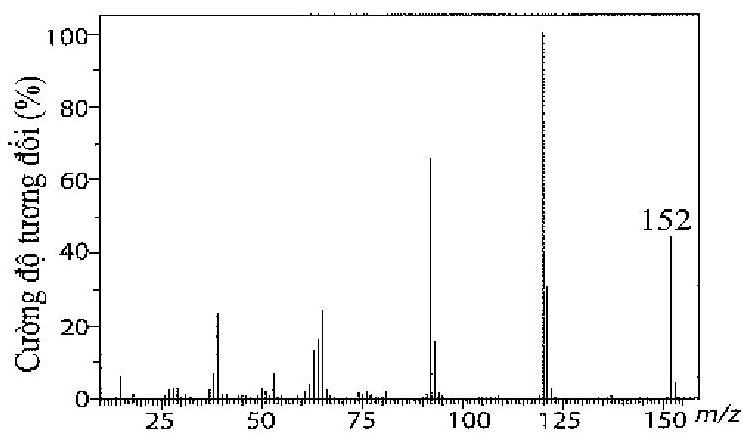
\includegraphics[width=\textwidth]{2025_10_23_f2823ef970776205e47bg-32}
\captionsetup{labelformat=empty}
\caption{Hìnli 10. Phổ MS của methyl salicylate}
\end{center}
\end{figure}

$10.13^{*}$. Lindane hay hexachlorane là chất có tác dụng trừ sâu mạnh, từng được sử dụng phổ biến trong nông nghiệp và làm dược phẩm (trị ghẻ, diệt chấy,...). Tuy nhiên, do là chất độc phân huỷ rất chậm trong tự nhiên nên vào năm 2009, hexachlorane đã bị đưa vào phụ lục cấm sản xuất và sử dụng của Công ước Stockholm về các chất ô nhiễm hữu cơ khó phân huỷ và bị cấm sữ dụng tại 169 quốc gia trên thế giới. Thành phần phần trăm khối lượng của các nguyên tố có trong hexachlorane là: $24,78 \% \mathrm{C} ; 2,08 \% \mathrm{H}$ và $73,14 \% \mathrm{Cl}$. Dựa vào phổ MS , xác định được phân tử khối của hexachlorane là 288 (ứng với ${ }^{35} \mathrm{Cl}$ ) hoặc 300 (ứng với ${ }^{37} \mathrm{Cl}$ ). Trong tự nhiên, ${ }^{35} \mathrm{Cl}$ chiếm $75,77 \%$ số lượng nguyên tử còn ${ }^{37} \mathrm{Cl}$ chiếm $24,23 \%$ số lượng nguyên tử.\\
a) Xác định công thức thực nghiệm của hexachlorane.\\
b) Xác định công thức phân tử của hexachlorane.

\section*{BAI 11}
CẤU TAO HOÁ HOC CỦA HỘP CHÁT HỮU COC\\
11.1. Để viết được cấu tạo hoá học của một chất cần biết những yếu tố nào sau đây?\\
(a) Thành phần phân tử của chất.\\
(b) Hoá trị của các nguyên tố có trong phân tử chất.\\
(c) Trật tự liên kết của các nguyên tử trong phân tử chất.\\
(d) Nhiệt độ sôi của chất.\\
11.2. Công thức nào dưới đây biểu diễn đúng cấu tạo hoá học của chất?\\
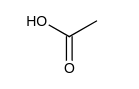
\includegraphics{smile-9000b27412d205ecfecaef73471a400232ff3abb}\\
(1)\\
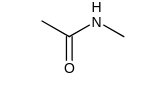
\includegraphics{smile-0c114765a9fce6331c4c2db89276fe2851534cd4}\\
(2)\\
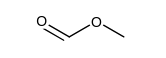
\includegraphics{smile-a0dbca82130c0164dadcb9ebb08c53d61f06568e}\\
(3)\\
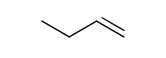
\includegraphics{smile-f0e852ad23e0cdece8a256de9af0bb0d2f954728}\\
(4)\\
A. Công thức (1).\\
B. Công thức (2) và công thức (3).\\
C. Công thức (4).\\
D. Công thức (1) và công thức (3).\\
11.3. Nhận xét nào sau đây là đúng về hai công thức cấu tạo $\mathrm{CH}_{3} \mathrm{CH}_{2} \mathrm{CH}\left(\mathrm{CH}_{3}\right)_{2}$ và $\mathrm{CH}_{3} \mathrm{CH}_{2} \mathrm{CH}_{2} \mathrm{CH}_{2} \mathrm{CH}_{3}$ ?\\
A. Biểu diễn cấu tạo hoá học của cùng một chất.\\
B. Biểu diễn cấu tạo hoá học của hai chất đồng phân về vị trí nhóm chức.\\
C. Biểu diễn cấu tạo hoá học của hai chất thuộc cùng dãy đồng đẳng.\\
D. Biểu diễn cấu tạo hoá học của hai chất đồng phân về mạch carbon.\\
11.4. Nhận xét nào sau đây về hai công thức cấu tạo bên là đúng?\\
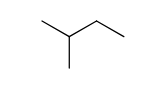
\includegraphics{smile-382ddbb66cbce9dafe6fc6503a49effc6ccd79c0}\\
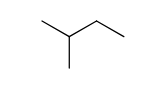
\includegraphics{smile-98adf0a9ce924f3d6d9b8d955c02327cef4b3a24}\\
A. Biểu diễn cấu tạo hoá học của hai chất đồng phân về mạch carbon.\\
B. Biểu diễn cấu tạo hoá học của hai chất đồng phân về vị trí nhóm chức.\\
C. Biểu diễn cấu tạo hoá học của hai chất thuộc cùng dãy đồng đẳng.\\
D. Biểu diễn cấu tạo hoá học của cùng một chất.\\
11.5. Chọn phát biểu đúng về bốn chất (đều có phân tử khối là 60 ) sau đây.\\
$\mathrm{CH}_{3} \mathrm{CH}_{2} \mathrm{CH}_{2} \mathrm{OH}$\\
(1)\\
$\underset{\text { O }}{\mathrm{CH}_{3} \mathrm{C}-\mathrm{OH}}$\\
(2)\\
$\mathrm{NH}_{2} \mathrm{CH}_{2} \mathrm{CH}_{2} \mathrm{NH}_{2}$\\
(3)\\
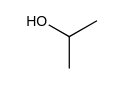
\includegraphics{smile-27287e9c228b535dfc34387348ef0576563872c2}\\
(4)\\
A. Chất (1) và chất (4) là đồng phân của nhau.\\
B. Chất (1), chất (2) và chất (4) là đồng phân của nhau.\\
C. Chất (1) và chất (2) là đồng phân của nhau.\\
D. Cả bốn chất đều là đồng phân của nhau.\\
11.6. Số đồng phân mạch hở có cùng công thức phân tử $\mathrm{C}_{3} \mathrm{H}_{6} \mathrm{Br}_{2}$ là\\
A. 1 .\\
B. 2 .\\
C. 3 .\\
D. 4 .\\
11.7. Methanol, ethanol, propanol, butanol thuộc cùng một dãy đồng đẳng. Phát biếu nào sau đây về các hợp chất này là đúng?\\
A. Các hợp chất này có tính chất vật lí tương tự nhau và có tính chất hoá học biến đổi theo quy luật.\\
B. Các hợp chất này có tính chất hoá học tương tự nhau và có tính chất vật lí biến đổi theo quy luật.\\
C. Các hợp chất này có cùng công thức phân tử nhưng có các tính chất vật lí, tính chất hoá học khác nhau.\\
D. Các hợp chất này có các tính chất vật lí và tính chất hoá học tương tự nhau.\\
11.8. Điền các thông tin thích hợp vào Ô trống để hoàn thành bảng dưới đây:

\begin{center}
\begin{tabular}{|l|l|l|l|}
\hline
Tên nihoum chúre & Ten chát hiriu cor & Công thưc cáu tao thu gon & Cong thire khung phin tir \\
\hline
Alkene & But-2-ene & $\mathrm{CH}_{3} \mathrm{CH}=\mathrm{CHCH}_{3}$ & 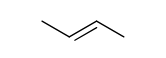
\includegraphics{smile-a75d4ea55ceb765b8cf310a69a3fb895b014b2ad} \\
\hline
Alcohol & Butan-1-ol & $\mathrm{CH}_{3} \mathrm{CH}_{2} \mathrm{CH}_{2} \mathrm{CH}_{2} \mathrm{OH}$ & ...(1)... \\
\hline
$\ldots$ (2) $\ldots$ & Propanal & $\mathrm{CH}_{3} \mathrm{CH}_{2} \mathrm{CHO}$ & ...(3)... \\
\hline

\includegraphics[max width=\textwidth]{2025_10_23_f2823ef970776205e47bg-34}
 & Pentanoic acid & 
\includegraphics[max width=\textwidth]{2025_10_23_f2823ef970776205e47bg-34(2)}
 & 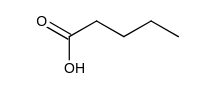
\includegraphics{smile-f826611fde2ef2ec56539e6c2d9d70082612bbfc} \\
\hline
$\ldots(6) \ldots$ & Ethyl propanoate & 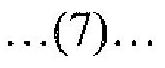
\includegraphics[max width=\textwidth]{2025_10_23_f2823ef970776205e47bg-34(1)}
 & 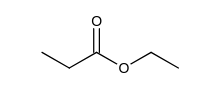
\includegraphics{smile-8e967ac8db62847f9fb82e1befe14ab2c654fc0a} \\
\hline
...(8)... & Pentylamine & $\mathrm{CH}_{3} \mathrm{CH}_{2} \mathrm{CH}_{2} \mathrm{CH}_{2} \mathrm{CH}_{2} \mathrm{NH}_{2}$ & $\ldots$ (9)... \\
\hline
\end{tabular}
\end{center}

11.9. Viết công thức cấu tạo của các hợp chất hữu cơ mạch hở có công thức phân tử $\mathrm{C}_{4} \mathrm{H}_{10} \mathrm{O}$. Trong các hợp chất này, hãy chỉ ra:\\
a) Các chất là đồng phân về nhóm chức.\\
b) Các chất là đồng phân về vị trí nhóm chức.\\
c) Các chất là đồng phân về mạch carbon.\\
11.10. Trong các công thức cấu tạo dưới đây:\\
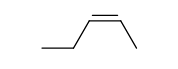
\includegraphics{smile-71f6c89f7bd7f7deee83e522e694f2b96a8b3e46}

(1)\\
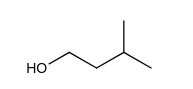
\includegraphics{smile-0eee30f118834fe0e15d7279ba8f506929f01d33}

(2)\\
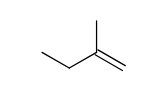
\includegraphics{smile-acf20f252aaefb5089ca8380a28675f725933ab8}

(3)\\
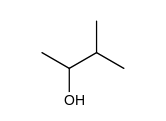
\includegraphics{smile-ff2fc8e37372b6da30bd465d5a37ed01411c4efb}

(4)\\
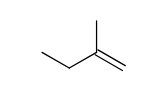
\includegraphics{smile-3f9d830d7f197ce110a24261f7f7614e2b471d64}

(5)\\
a) Những công thức nào biểu diễn công thức cấu tạo của cùng một chất?\\
b) Những công thức nào biểu diễn công thức cấu tạo của hai chất là đồng phân của nhau? Hai chất đồng phân này thuộc loại đồng phân gi (đồng phân về mạch carbon, đồng phân về nhóm chức hay đồng phân về vị trí nhóm chức)?\\
11.11. Hai chất đầu trong các chất thuộc một số dãy đồng đẳng được cho dưới đây:

Dãy 1: $\mathrm{CH}_{2} \mathrm{O}, \mathrm{C}_{2} \mathrm{H}_{4} \mathrm{O}$.\\
Dãy 2: $\mathrm{C}_{2} \mathrm{H}_{3} \mathrm{~N}, \mathrm{C}_{3} \mathrm{H}_{5} \mathrm{~N}$.\\
Dãy 3: $\mathrm{C}_{6} \mathrm{H}_{6}, \mathrm{C}_{7} \mathrm{H}_{8}$.\\
a) Viết công thức phân tử của chất thứ 5 trong mỗi dãy.\\
b) Viết công thức chung cho mỗi dãy.\\
11.12. Các hợp chất $\mathrm{CH}_{3} \mathrm{COOH}\left(\mathrm{C}_{2} \mathrm{H}_{4} \mathrm{O}_{2}\right), \mathrm{HOCH}_{2} \mathrm{CH}_{2} \mathrm{CHO}\left(\mathrm{C}_{3} \mathrm{H}_{6} \mathrm{O}_{2}\right)$ và $\mathrm{CH}_{3} \mathrm{CH}_{2} \mathrm{COOCH}_{3}\left(\mathrm{C}_{4} \mathrm{H}_{8} \mathrm{O}_{2}\right)$ có thuộc cùng một dãy đồng đẳng không? Vì sao? Viết công thức cấu tạo của ba chất có cùng công thức phân tử với các chất ở trên và là đồng đẳng của nhau.\\
11.13. Một hợp chất hữu cơ A được xác định có công thức thực nghiệm là $\mathrm{CH}_{2} \mathrm{O}$.\\
a) Các nguyên tố nào có trong thành phần phân tử của A ?\\
b) Bằng phổ MS , người ta xác định được phân tử khối của A là 60 . Tìm công thức phân tử của $\mathbf{A}$.\\
c) Trên phổ IR của A thấy có tín hiệu hấp thự ở $1715 \mathrm{~cm}^{-1}$ đồng thời cũng thấy một số tín hiệu hấp thụ trong vùng $3400-2500 \mathrm{~cm}^{-1}$. A có thể có nhóm chức nào? Xác định công thức cấu tạo của $\mathbf{A}$.\\
11.14. Thành phần phần trăm về khối lượng nguyên tố có trong hợp chất X là $85,7 \%$ C và $14,3 \%$ H.\\
a) Xác định công thức thực nghiệm của hợp chất X .\\
b) Phổ MS cho thấy X có phân tử khối là 56. Xác định công thức phân tử của X.\\
c) Cho biết công thức cấu tạo có thể có của X trong mỗi trường hợp:\\
c1) X là hydrocarbon mạch thẳng.\\
c2) X là hydrocarbon mạch hở, phân nhánh.

\section*{CHỦ DỀ 4 HYDROCARBON}
\section*{BAT}
\section*{ALKANE}
12.1. Phát biểu nào sau đây là đúng?\\
A. Những hợp chất mà trong phân đử chỉ có liên kết đơn là hydrocarbon no.\\
B. Hydrocarbon chỉ có liên kết đơn trong phân tử là hydrocarbon no.\\
C. Hydrocarbon có các liên kết đơn trong phân tử là hydrocarbon no.\\
D. Hydrocarbon có ít nhất một liên kết đơn trong phân tử là hydrocarbon no.\\
12.2. Phát biểu nào sau đây về alkane là không đúng?\\
A. Trong phân tử alkane chỉ có liên kết đơn.\\
B. Chỉ các alkane là chất khí ở điều kiện thường được dùng làm nhiên liệu.\\
C. Các alkane lỏng được dùng sản xuất xăng, dầu và làm dung môi.\\
D. Các alkane rắn được dùng làm nhựa đường, nguyên liệu cho quá trình cracking.\\
E. Công thức chung của alkane là $\mathrm{C}_{\mathrm{x}} \mathrm{H}_{2 \mathrm{x}+2}$, với $\mathrm{x} \geq 1$.\\
12.3. Số đồng phân cấu tạo ứng với công thức phân tử $\mathrm{C}_{6} \mathrm{H}_{14}$ là\\
A. 3 .\\
B. 5.\\
C. 4 .\\
D. 6 .\\
12.4. Tên thay thế của hydrocarbon có công thức cấu tạo $\left(\mathrm{CH}_{3}\right)_{3} \mathrm{CCH}_{2} \mathrm{CH}_{2} \mathrm{CH}_{3}$ là\\
A. 2,2-dimethylpentane.\\
B. 2,3-dimethylpentane.\\
C. 2,2,3-trimethylbutane.\\
D. 2,2-dimethylbutane.\\
12.5. Những yếu tố nào sau đây không quyết định đến độ lớn của nhiệt độ sôi của các alkane?\\
(a) Phân tữ khối.\\
(b) Tương tác van der Waals giữa các phân tử.\\
(c) Độ tan trong nước.\\
(d) Liên kết hydrogen gữa các phân tử.\\
12.6. Khi dehydrogen hợp chất 2,3-dimethylbutane có thế thu được bao nhiêu alkene đồng phân cấu tạo của nhau?\\
A. 3 .\\
B. 4 .\\
C. 2 .\\
D. 5 .\\
12.7. Cho nhiệt đốt cháy hoàn toàn 1 mol các chất ethane, propane, butane và pentane lần lượt là $1570 \mathrm{~kJ} \mathrm{~mol}^{-1} ; 2220 \mathrm{~kJ} \mathrm{~mol}^{-1} ; 2875 \mathrm{~kJ} \mathrm{~mol}^{-1}$ và $3536 \mathrm{~kJ} \mathrm{~mol}^{-1}$. Khi đốt cháy hoàn toàn 1 gam chất nào sẽ thu được lượng nhiệt lớn nhất?\\
A. Ethane.\\
B. Propane.\\
C. Pentane.\\
D. Butane.\\
12.8. Nhỏ 1 mL nước bromine vào ống nghiệm đựng 1 mL hexane, chiếu sáng và lắc đều. Hiện tượng quan sát được là\\
A. trong ống nghiệm có chất lỏng đồng nhất.\\
B. màu của nước bromine bị mất.\\
C. màu của bromine không thay đồi.\\
D. trong ống nghiệm xuất hiện kết tủa.\\
12.9. Hydrocarbon $Y$ có công thức cấu tạo như sau: $\left(\mathrm{CH}_{3}\right)_{2} \mathrm{CHCH}_{2} \mathrm{CH}_{3}$. Khi cho Y phản ứng với bromine có thể thu được bao nhiêu dẫn xuất monobromo là đồng phân cấu tạo của nhau?\\
A. 3 .\\
B. 4 .\\
C. 5.\\
D. 6 .\\
12.10. Trong phân tử hydrocarbon $X$, hydrogen chiếm $25 \%$ về khối lượng. Công thức phân tử của X là\\
A. $\mathrm{CH}_{4}$.\\
B. $\mathrm{C}_{2} \mathrm{H}_{4}$.\\
C. $\mathrm{C}_{2} \mathrm{H}_{6}$.\\
D. $\mathrm{C}_{6} \mathrm{H}_{6}$.\\
12.11. Cho butane phản ứng với chlorine thu được sản phẩm chính là\\
A. 2-chlorobutane.\\
B. 1-chlorobutane.\\
C. 3-chlorobutane.\\
D. 4-chlorobutane.\\
12.12. Để tăng chất lượng của xăng, dầu, người ta thực hiện cách nào sau đây?\\
A. Thực hiện phản úng reforming để thay đồi cấu trúc của các alkane mạch không nhánh thành hydrocarbon mạch nhánh hoặc mạch vòng có chỉ số octane cao.\\
B. Thực hiện phản ứng cracking để thay đổi cấu trúc các alkane mạch dài chuyển thành các alkene và alkane mạch ngắn hơn.\\
C. Thực hiện phản úng hydrogen hoá để chuyển các alkene thành alkane.\\
D. Bổ sung thêm heptane vào xăng, dầu.\\
12.13. Phương pháp nào sau đây có thể được thực hiện để góp phần hạn chế ô nhiễm môi trường do các phương tiện giao thông gây ra?\\
A. Không sử dụng phương tiện giao thông.\\
B. Cấm các phương tiện giao thông tại các đô thị.\\
C. Sử dụng phương tiện chạy bằng điện hoặc nhiên liệu xanh.\\
D. Sử dụng các phương tiện chạy bằng than đá.\\
12.14. Trong công nghiệp, các alkane được điểu chế từ nguồn nào sau đây?\\
A. Sodium acetate.\\
B. Dầu mỏ và khí mỏ dầu.\\
C. Aluminium carbide $\left(\mathrm{Al}_{4} \mathrm{C}_{3}\right)$.\\
D. Khí biogas.\\
12.15. Trong phản ứng thế nguyên tữ H của phân tử alkane, bromine có tính chọn lọc cao, nghĩa là xác suất thế nguyên tử H ở nguyên tử carbon bậc ba gấp hàng trăm lần xác suất thế H ở nguyên tử carbon bậc một và bậc hai. Xác định công thức cấu tạo sản phẩm chính của phản ứng xảy ra khi cho $\left(\mathrm{CH}_{3}\right)_{2} \mathrm{CHCH}_{2} \mathrm{CH}_{3}$ phản úng với bromine (chiếu sáng).\\
12.16. Viết công thức cấu tạo của các hợp chất không no có thể thu được khi thực hiện phản ứng tách một phân tử hydrogen từ phân tữ 2-methylbutane.\\
12.17. Trong quá trình khai thác hoặc vận chuyển dầu mỏ, đôi khi xảy ra sự cố tràn dầu trên biển.\\
a) Các sự cố tràn dầu trên biển gây ra các thảm hoạ về môi trường như thế nào?\\
b) Để xử lí sự cố tràn dầu trên biển, người ta thường làm như thế nào? Giải thích lí do sử dụng các kĩ thuật đó.\\
12.18*. "Băng cháy" là dạng tinh thể hydrate của methane với nước, có công thức là $\mathrm{CH}_{4} \cdot \mathrm{nH}_{2} \mathrm{O}$. Băng cháy được hình thành ở sâu dưới lòng đất dưới đáy biển và là nguồn methane quan trọng trong tương lai. Em hảy đề xuất biện pháp khai thác băng cháy.\\
12.19. Xăng làm nhiên liệu cho ô tô, xe máy là hỗn hợp của các hydrocarbon mạch nhánh $\mathrm{C}_{5} \mathrm{H}_{12}-\mathrm{C}_{11} \mathrm{H}_{24}$, trong đó có octane là chất có khả năng chịu kích nổ tốt. Vi sao người ta không dùng một loại hydrocarbon (ví dụ octane) đề làm xăng mà lại dùng hỗn hợp các hydrocarbon?\\
12.20. Khi đốt cháy 1 mol các chất sau đây giải phóng ra nhiệt lượng (gọi là nhiệt đốt cháy) như bảng sau:

\begin{center}
\begin{tabular}{|l|l|l|l|}
\hline
Chát & Nhiét luquig (lid mol-1) & Chát & Nhiét living (kil mol ${ }^{-1}$ ) \\
\hline
methane & 783 & propane & 2220 \\
\hline
ethane & 1570 & butane & 2875 \\
\hline
\end{tabular}
\end{center}

a) Khi đốt 1 gam chất nào sẽ giải phóng ra lượng nhiệt lớn nhất?\\
b) Dể đun sôi cùng một lượng nước từ cùng nhiệt độ ban đầu, với giả thiết các điều kiện khác là như nhau, cần đốt cháy khối lượng chất nào là ít nhất?\\
12.21. Khí đốt hoá lỏng (Liquified Petroleum Gas, viết tắt là LPG) hay còn được gọi là gas, là hỗn hợp khí chủ yếu gồm propane $\left(\mathrm{C}_{3} \mathrm{H}_{8}\right)$ và butane $\left(\mathrm{C}_{4} \mathrm{H}_{10}\right)$ đã được hoá lóng. Một loại gas dân dụng chứa khí hoá lỏng có tỉ lệ mol propane : butane là $40: 60$. Đốt cháy 1 lít khí gas này ( $0^{3} 25^{\circ} \mathrm{C}, 1$ bar) thì toả ra một lượng nhiệt bằng bao nhiêu? Biết khi đốt cháy 1 mol mỗi chất propane và butane toả ra lượng nhiệt tương ứng 2220 kJ và 2875 kJ .\\
12.22. Khí gas đun nấu có thể gây ngạt. Khí gas nặng hon không khí (propane nặng gấp 1,55 lần; butane nặng gấp 2,07 lần không khí) nên khi thoát khỏi thiết bị chứa, gas tích tụ ở những chỗ thấp trên mặt đất và tạo thành hỗn hợp gây cháy nổ. Khi phát hiện rò rỉ khí gas trong nhà, chúng ta cần phải làm gì để đảm bảo an toàn?\\
12.23. Vì sao nói "Các phương tiện giao thông là một trong các nguyên nhân chính gây ra ô nhiễm môi trường ở các đô thị lớn"?

\section*{BAI HYDROCARBON KHÔNG NO}
13.1. Phát biểu nào sau đây là đúng?\\
A. Hydrocarbon không no là những hydrocarbon mạch hở, phân tử chỉ có liên kết đôi $\mathrm{C}=\mathrm{C}$ hoặc liên kết ba $\mathrm{C}=\mathrm{C}$.\\
B. Hydrocarbon không no là những hydrocarbon mạch vòng, phân tử có liên kết đôi $\mathrm{C}=\mathrm{C}$ hoặc liên kết ba $\mathrm{C} \equiv \mathrm{C}$.\\
C. Hydrocarbon không no là những hydrocarbon mạch hở, phân tử có liên kết đôi $\mathrm{C}=\mathrm{C}$ hoặc liên kết ba $\mathrm{C} \equiv \mathrm{C}$.\\
D. Hydrocarbon không no là những hydrocarbon trong phân tữ có chứa liên kết đôi $\mathrm{C}=\mathrm{C}$ hoặc liên kết ba $\mathrm{C}=\mathrm{C}$ hoặc cả hai loại liên kết đó.\\
13.2. Phát biểu nào sau đây là không đúng?\\
A. Công thức chung của các hydrocarbon không no, mạch hở, phân tử có một liên kết đôi $\mathrm{C}=\mathrm{C}$ là $\mathrm{C}_{\mathrm{n}} \mathrm{H}_{2 \mathrm{n}}, \mathrm{n} \geq 2$.\\
B. Công thức phân tử của các hydrocarbon không no, mạch hở, phân tữ có một liên kết ba $\mathrm{C} \equiv \mathrm{C}$ có dạng $\mathrm{C}_{\mathrm{n}} \mathrm{H}_{2 \mathrm{n}-2}, \mathrm{n} \geq 2$.\\
C. Công thức phân tử của các hydrocarbon no, mạch hở có dạng $\mathrm{C}_{\mathrm{n}} \mathrm{H}_{2 \mathrm{n}}, \mathrm{n} \geq 2$.\\
D. Công thức chung của các hydrocarbon là $\mathrm{C}_{\mathrm{x}} \mathrm{H}_{\mathrm{y}}$ với $\mathrm{x} \geq 1$.\\
13.3. Cho các chất có công thức cấu tạo sau: (1) $\mathrm{ClCH}_{2} \mathrm{CH}=\mathrm{CHCH}_{3}$; (2) $\mathrm{CH}_{3} \mathrm{CH}=\mathrm{CHCH}_{3}$;\\
(3) $\mathrm{BrCH}_{2} \mathrm{C}\left(\mathrm{CH}_{3}\right)=\mathrm{C}\left(\mathrm{CH}_{2} \mathrm{CH}_{3}\right)_{2}$; (4) $\mathrm{ClCH}_{2} \mathrm{CH}=\mathrm{CH}_{2}$; (5) $\mathrm{ClCH}_{2} \mathrm{CH}=\mathrm{CHCH}_{2} \mathrm{CH}_{3}$;\\
(6) $\left(\mathrm{CH}_{3}\right)_{2} \mathrm{C}=\mathrm{CH}_{2}$. Trong số các chất trên, bao nhiêu chất có đồng phân hình học?\\
A. 3 .\\
B. 4 .\\
C. 5.\\
D. 6 .\\
13.4. Cho các alkene $X$ và $Y$ có công thức như sau:

(X)\\
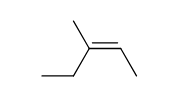
\includegraphics{smile-51e0713fbb70a71d230f7f66d15d00afcb4f8e10}

(Y)\\
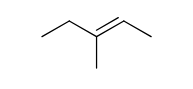
\includegraphics{smile-41cb7f119ed15881f93112ef4b6ef8c90d4fd45d}

Tên gọi của $X$ và $Y$ tương ứng là\\
A. cis-3-methylpent-2-ene và trans-3-methylpent-3-ene.\\
B. trans-3-methylpent-2-ene và cis-3-methylpent-2-ene.\\
C. trans-3-methylpent-3-ene và cis-3-methylpent-3-ene.\\
D. trans-3-methylpent-3-ene và cis-3-methylpent-2-ene.\\
13.5. Các alkene không có các tính chất vật lí đặc trưng nào sau đây?\\
A. Tan tốt trong nước và các dung môi hữu cơ.\\
B. Có khối lượng riêng nhỏ hơn khối lượng riêng của nước.\\
C. Có nhiệt độ sôi thấp hơn alkane phân tử có cùng số nguyên tử carbon.\\
D. Không dẫn điện.\\
13.6. Một hydrocarbon X mạch hở trong phân tử có phần trăm khối lượng carbon bằng $85,714 \%$. Trên phổ khối lượng của $\mathbf{X}$ có peak ion phân tử ứng với giá trị $m / z=42$. Công thức phù hợp với X là\\
A. $\mathrm{CH}_{2}=\mathrm{CHCH}_{3}$.\\
B. $\mathrm{CH}_{3} \mathrm{CH}_{2} \mathrm{CH}_{3}$. -\\
C. $\mathrm{CH}_{3} \mathrm{CH}_{3}$.\\
D. $\mathrm{CH} \equiv \mathrm{CH}$.\\
13.7. But-1-ene tác dụng với HBr tạo ra sản phẩm chính có công thức cấu tạo nào sau đây?\\
A. $\mathrm{CH}_{3} \mathrm{CHBrCHBrCH} 3$.\\
B. $\mathrm{CH}_{3} \mathrm{CH}_{2} \mathrm{CH}_{2} \mathrm{CH}_{2} \mathrm{Br}$.\\
C. $\mathrm{CH}_{3} \mathrm{CH}_{2} \mathrm{CHBrCH}_{3}$.\\
D. $\mathrm{BrCH}_{2} \mathrm{CH}_{2} \mathrm{CH}_{2} \mathrm{CH}_{2} \mathrm{Br}$.\\
13.8. Cho các hydrocarbon: (1) $\mathrm{CH}_{2}=\mathrm{C}\left(\mathrm{CH}_{3}\right) \mathrm{CH}_{2} \mathrm{CH}_{3}$; (2) $\left(\mathrm{CH}_{3}\right)_{2} \mathrm{C}=\mathrm{CHCH}_{3}$; (3) $\mathrm{CH}_{2}=\mathrm{C}\left(\mathrm{CH}_{3}\right) \mathrm{CH}=\mathrm{CH}_{2}$; (4) $\left(\mathrm{CH}_{3}\right)_{2} \mathrm{CHC} \equiv \mathrm{CH}$. Những hydrocarbon nào phản ứng với HBr sinh ra sản phẩm chính là 2-bromo-2-methylbutane?\\
A. (1) và (2).\\
B. (2) và (4).\\
C. (1) và (3).\\
D. (3) và (4).\\
13.9. Cho pent-2-ene phản ứng với dung dịch $\mathrm{KMnO}_{4}$ ở nhiệt độ phòng có thể thu được sản phẩm hữu cơ có công thức cấu tạo nào sau đây?\\
A. $\mathrm{CH}_{3} \mathrm{CH}_{2} \mathrm{CH}(\mathrm{OH}) \mathrm{CH}(\mathrm{OH}) \mathrm{CH}_{3}$.\\
B. $\mathrm{CH}_{3} \mathrm{CH}_{2} \mathrm{CH}_{2} \mathrm{CH}(\mathrm{OH}) \mathrm{CH}_{3}$.\\
C. $\mathrm{CH}_{3} \mathrm{CH}(\mathrm{OH}) \mathrm{CH}_{2} \mathrm{CH}(\mathrm{OH}) \mathrm{CH}_{3}$.\\
D. $\mathrm{CH}_{3} \mathrm{CH}_{2} \mathrm{CH}(\mathrm{OH}) \mathrm{CH}_{2} \mathrm{CH}_{3}$.\\
13.10. Dẫn dòng khí gồm acetylene và ethylene lần lượt đi vào ống nghiệm (1) đựng dung dịch $\mathrm{AgNO}_{3} / \mathrm{NH}_{3}$ ở điều kiện thường, sau đó dẫn tiếp qua ống nghiệm (2) đựng nước bromine. Hiện tượng thí nghiệm nào sau đây là không đúng?\\
A. Ở ống nghiệm (1) có kết tủa màu vàng nhạt.\\
B. Ở ống nghiệm (2) màu của nước bromine nhạt dần.\\
C. Ở ống nghiệm (2) chất lỏng chia thành hai lớp.\\
D. Ở ống nghiệm (2) thu được chất lỏng đồng nhất.\\
13.11. Dể phân biệt but-2-yne $\left(\mathrm{CH}_{3} \mathrm{C} \equiv \mathrm{CCH}_{3}\right)$ với but-1-yne $\left(\mathrm{CH} \equiv \mathrm{CCH}_{2} \mathrm{CH}_{3}\right)$ có thể dùng thuốc thử nào sau đây?\\
A. Dung dịch HCl .\\
B. Dung dịch $\mathrm{AgNO}_{3} / \mathrm{NH}_{3}$,\\
C. Nước bromine.\\
D. Dung dịch $\mathrm{KMnO}_{4}$.\\
13.12. Các chai lọ, túi, màng mỏng trong suốt, không độc, được sử dụng làm chai đựng nước, thực phẩm, màng bọc thực phẩm được sản xuất từ polymer của chất nào sau đây?\\
A. Butadiene.\\
B. Propene.\\
C. Vinyl chloride.\\
D. Ethylene.\\
13.13. Phát biểu nào sau đây là không đúng?\\
A. Trong phòng thí nghiệm, người ta điều chế ethene bằng cách tách nước ethanol và thu bằng cách dời chỗ của nước.\\
B. Một ứng dụng quan trọng của acetylene là làm nhiên liệu trong đèn xì oxygen -- acetylene.\\
C. Trong công nghiệp, người ta điều chế acetylene bằng cách nhiệt phân nhanh methane có xúc tác hoặc cho calcium carbide (thành phần chính của đất đèn) tác dụng với nước.\\
D. Một úng dụng quan trọng của acetylene là làm nguyên liệu tổng hợp ethylene.\\
13.14. Viết công thức cấu tạo và gọi tên các alkene đồng phân cấu tạo có công thức phân tử $\mathrm{C}_{5} \mathrm{H}_{10}$. Trong số các đồng phân này, có bao nhiêu chất có đồng phân hình học? Hây viết tên đầy đủ của các đồng phân hình học này.\\
13.15. Nhiệt đốt cháy của một số chất như sau: ethane: $1570 \mathrm{~kJ} \mathrm{~mol}^{-1}$; methane: $783 \mathrm{~kJ} \mathrm{~mol}^{-1}$; acetylene: $1300 \mathrm{~kJ} \mathrm{~mol}^{-1}$. Vì sao trong hàn, cắt kim loại, người ta dùng acetylene được điều chế từ calcium carbide $\mathrm{CaC}_{2}$ (thành phần chính của đất đèn) mà không dùng ethane?\\
13.16*. Trước đây, công nghiệp hoá học hữu cơ sử dụng rất nhiều acetylene làm nguyên liệu đầu. Ngày nay, acetylene được thay thế bằng ethylene. Hãy tìm hiểu và giải thích lí do của sự thay đồi này.\\
13.17. Khi sục hai dòng khí như nhau của ethylene và acetylene vào dung dịch $\mathrm{KMnO}_{4}$ thấy ethylene làm nhạt màu dung dịch nhanh hon acetylene. Hãy giải thích nguyên nhân.\\
13.18. Một số hydrocarbon mạch hở, đồng phân cấu tạo của nhau, trong phân tử có phần trăm khối lượng carbon bằng $85,714 \%$. Trên phổ khối lượng của một trong các chất trên có peak ion phân tứ úng với giá trị $m / z=70$. Viết công thức cấu tạo của các chất thoả măn các đặc điểm trên.

\section*{$3 \times 1$ 14 ARENE (HYDROCARBON THÓM)}
14.1. Phát biểu nào sau đây là không đúng?\\
A. Hydrocarbon thơm là những hydrocarbon trong phân tử có vòng benzene.\\
B. Các chất trong phân tử có vòng benzene được gọi là hydrocarbon thơm.\\
C. Những hydrocarbon trong phân tử có vòng benzene được gọi là hydrocarbon thom.\\
D. Dãy đồng đẳng của benzene có công thức tổng quát $\mathrm{C}_{\mathrm{n}} \mathrm{H}_{2 \mathrm{n}-6}(\mathrm{n} \geq 6)$.\\
14.2. Cho các hydrocarbon X và Y có công thức cấu tạo sau:\\
Tên gọi của $X$ và $Y$ lần lượt là\\
A. $p$-xylene và $m$-xylene.\\
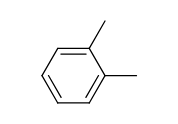
\includegraphics{smile-e339a7316f6c6d22d6a7c5aa58b33e25d442896f}

(X)\\
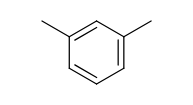
\includegraphics{smile-478bfd0257a29f6b3a247b3940bf80fb4652db95}

(Y)\\
B. 1,2-dimethylbenzene và 1,3-dimethylbenzene.\\
C. $m$-xylene và $o$-xylene.\\
D. 1,3-dimethylbenzene và 1,2-dimethylbenzene.\\
14.3. Một arene $Y$ có phần trăm khối lượng carbon bằng $92,307 \%$. Trên phổ khối lượng của $\mathbf{Y}$ có peak ion phân tử ứng với giá trị $m / z=104$. Công thức cấu tạo phân tử của $Y$ là\\
A. $\mathrm{C}_{6} \mathrm{H}_{5} \mathrm{CH}=\mathrm{CH}_{2}$.\\
B. $\mathrm{CH}_{3} \mathrm{C}_{6} \mathrm{H}_{4} \mathrm{CH}_{3}$.\\
C. $\mathrm{C}_{6} \mathrm{H}_{5} \mathrm{C} \equiv \mathrm{CH}$.\\
D. $\mathrm{C}_{6} \mathrm{H}_{5} \mathrm{C}_{2} \mathrm{H}_{5}$.\\
14.4. Phát biểu nào sau đây là không đúng?\\
A. Toluene ( $\mathrm{C}_{6} \mathrm{H}_{5} \mathrm{CH}_{3}$ ) không tác dụng được với nước bromine, dung dịch thuốc tím ở điều kiện thường.\\
B. Styrene $\left(\mathrm{C}_{6} \mathrm{H}_{5} \mathrm{CH}=\mathrm{CH}_{2}\right)$ tác dụng được với nước bromine, làm mât màu dung dịch thuốc tím ở điều kiện thường.\\
C. Ethylbenzene ( $\mathrm{C}_{6} \mathrm{H}_{5} \mathrm{CH}_{2} \mathrm{CH}_{3}$ ) không tác dụng được với nước bromine, làm mất màu dung dịch thuốc tím khi đun nóng.\\
D. Naphthalene $\left(\mathrm{C}_{10} \mathrm{H}_{8}\right)$ tác dụng được với nước bromine, làm mất màu dung dịch thuốc tím ở điều kiện thường.\\
14.5. Cho một số arene có công thức cấu tạo sau:\\
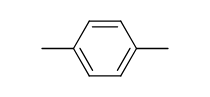
\includegraphics{smile-0154655c5f83b3260af9018489c100935dc1dbab}\\
(1)\\
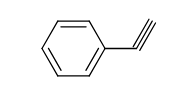
\includegraphics{smile-ff8505c1b846bfffff80f00c5e2bb34e2b64192c}\\
(2)\\
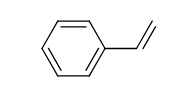
\includegraphics{smile-ffaee4009f589567f8e99f6615d66ac9f036ea17}\\
(3)\\
\includegraphics{smile-5eb588bb87722fd43233c483ce791c42dc84d3f6}\\
(4)\\
\includegraphics{smile-3bfee99718eea1d3979da4a966257ffb341658cf}\\
(5)\\
\includegraphics{smile-4fbbb59a86bf4057e79664aa6436ca23be8ea174}\\
(6)\\
\includegraphics{smile-0fcc33ffe38271124ca13c4e82231bb8d0cd77e3}\\
(7)

Trong số các chất trên, có bao nhiêu chất là đồng phân cấu tạo của nhau?\\
A. 2 .\\
B. 4 .\\
C. 6 .\\
D. 5 .\\
14.6. Phát biểu nào sau đây về quá trình sản xuất các hydrocarbon trong công nghiệp là không đúng?\\
A. Người ta có thể khai thác/ điều chế toluene bằng quá trình reforming hexane và heptane.\\
B. Người ta có thể khai thác/ điều chế toluene và benzene từ nhựa than đá.\\
C. Người ta có thể khai thác/ điều chế benzene bằng phản ứng trimer hoá acetylene.\\
D. Người ta có thể khai thác benzene từ dầu mỏ hoặc điều chế benzene bằng phản ứng reforming hexane.\\
14.7. Chất lỏng X (có công thức phân tử là $\mathrm{C}_{6} \mathrm{H}_{6}$ ) không màu, có mùi thơm nhẹ, không tan trong nước, là một dung môi hữu cơ thông dụng. X tác dụng với chlorine khi chiếu sáng tạo nên chất rắn $\mathbf{Y}$; tác dụng với chlorine khi có xúc tác $\mathrm{FeCl}_{3}$ tạo ra chất lỏng $\mathbb{Z}$ và khí $\mathbb{T}$. Khí $\mathbb{T}$ khi đi qua dung dịch silver nitrate tạo ra kết tủa trắng. Công thức của các chất $\mathbb{Y}, \mathbb{Z}, \mathbb{T}$ lần lượt là\\
A. $\mathrm{C}_{6} \mathrm{H}_{6} \mathrm{Cl}_{6} ; \mathrm{C}_{6} \mathrm{H}_{5} \mathrm{Cl} ; \mathrm{HCl}$.\\
B. $\mathrm{C}_{6} \mathrm{H}_{5} \mathrm{Cl} ; \mathrm{C}_{6} \mathrm{H}_{6} \mathrm{Cl}_{6} ; \mathrm{HCl}$.\\
C. $\mathrm{C}_{6} \mathrm{H}_{5} \mathrm{Cl}_{5}\left(\mathrm{CH}_{3}\right) ; \mathrm{C}_{6} \mathrm{H}_{5} \mathrm{CH}_{2} \mathrm{Cl} ; \mathrm{HCl}$.\\
D. $\mathrm{C}_{6} \mathrm{H}_{5} \mathrm{CH}_{2} \mathrm{Cl} ; \mathrm{C}_{6} \mathrm{H}_{5} \mathrm{Cl}_{5}\left(\mathrm{CH}_{3}\right) ; \mathrm{HCl}$.\\
14.8. Chất nào sau đây khi đun nóng với dung dịch $\mathrm{KMnO}_{4} / \mathrm{H}_{2} \mathrm{SO}_{4}$ tạo thành hợp chất hữu cơ đơn chức?\\
A. $\mathrm{C}_{6} \mathrm{H}_{5} \mathrm{CH}_{3}$.\\
B. $m-\mathrm{CH}_{3} \mathrm{C}_{6} \mathrm{H}_{4} \mathrm{CH}_{3}$.\\
C. $o-\mathrm{CH}_{3} \mathrm{C}_{6} \mathrm{H}_{4} \mathrm{CH}_{3}$.\\
D. $p-\mathrm{CH}_{3} \mathrm{C}_{6} \mathrm{H}_{4} \mathrm{CH}_{3}$.\\
14.9. Để phân biệt styrene và phenylacetylene chỉ cần dùng. chất nào sau đây?\\
A. Nước bromine.\\
B. Dung dịch $\mathrm{KMnO}_{4}$.\\
C. Dung dịch $\mathrm{AgNO}_{3} / \mathrm{NH}_{3}$.\\
D. Khí oxygen dư.\\
14.10. Hydrocarbon thơm X có công thức phân tử $\mathrm{C}_{8} \mathrm{H}_{10}$, khi tác dụng với dưng dịch $\mathrm{KMnO}_{4}$ trong môi trường $\mathrm{H}_{2} \mathrm{SO}_{4}$ tạo nên hợp chất hữu cơ đơn chức $\mathcal{X}$. X phản ứng với chlorine có chiếu sáng tạo hợp chất hữu cơ $\mathbb{Z}$ chưa một nguyên tử Cl trong phân tử (là sản phẩm chính). Các chất $X, Y, Z$ có công thức cấu tạo lần lượt là\\
A. $\mathrm{C}_{6} \mathrm{H}_{5} \mathrm{CH}_{2} \mathrm{CH}_{3} ; \mathrm{C}_{6} \mathrm{H}_{5} \mathrm{COOH} ; \mathrm{C}_{6} \mathrm{H}_{5} \mathrm{CHClCH}_{3}$.\\
B. $\mathrm{C}_{6} \mathrm{H}_{5} \mathrm{CH}_{2} \mathrm{CH}_{3} ; \mathrm{C}_{6} \mathrm{H}_{5} \mathrm{CH}_{2} \mathrm{COOH} ; \mathrm{C}_{6} \mathrm{H}_{5} \mathrm{CHClCH}_{3}$.\\
C. $o-\mathrm{CH}_{3} \mathrm{C}_{6} \mathrm{H}_{4} \mathrm{CH}_{3} ; o-\mathrm{HOOCC}_{6} \mathrm{H}_{4} \mathrm{COOH} ; o-\mathrm{ClCH}_{2} \mathrm{C}_{6} \mathrm{H}_{4} \mathrm{CH}_{2} \mathrm{Cl}$.\\
D. $p-\mathrm{CH}_{3} \mathrm{C}_{6} \mathrm{H}_{4} \mathrm{CH}_{3} ; p-\mathrm{HOOCC} \mathrm{H}_{4} \mathrm{COOH} ; p-\mathrm{ClCH}_{2} \mathrm{C}_{6} \mathrm{H}_{4} \mathrm{CH}_{2} \mathrm{Cl}$.\\
14.11. Cho 30 mL dung dịch $\mathrm{HNO}_{3}$ đặc và 25 mL dung dịch $\mathrm{H}_{2} \mathrm{SO}_{4}$ đặc vào bình cầu ba cổ có lắp ống sinh hàn, phễu nhỏ giọt và nhiệt kế rồi làm lạnh hỗn họp đến $30^{\circ} \mathrm{C}$. Cho từng giọt benzene vào hỗn hợp phản ứng, đồng thời lắc đều và giữ nhiệt độ ở $60^{\circ} \mathrm{C}$ trong 1 giờ. Để nguội bình, sau đó rót hỗn hợp phản ứng vào phễu chiết, hỗn hợp tách thành hai lớp. Tách bỏ phần acid ở bên dưới. Rưa phần chất lỏng còn lại bằng dung dịch sodium carbonate, sau đó rửa bằng nước, thu được chất lỏng nặng hơn nước, có màu vàng nhạt. Kết luận nào sau đây về phản ứng trên là không đúng?\\
A. Chất lỏng màu vàng nhạt là nitrobenzene.\\
B. Sulfuric acid có vai trò chất xúc tác.\\
C. Đã xảy ra phản ứng thế vào vòng benzene.\\
D. Nitric acid đóng vai trò là chất oxi hoá.\\
14.12*. Một trong những ứng dụng của toluene là\\
A. làm phụ gia để tăng chỉ số octane của nhiên liệu.\\
B. làm chất đầu để sản xuất methylcyclohexane.\\
C. làm chất đầu để điều chế phenol.\\
D. làm chất đầu để sản xuất polystyrene.\\
14.13. Một số chất gây ô nhiễm môi trường như benzene, toluene có trong khí thải đốt cháy nhiên liệu xăng, dầu. Để giảm thiểu nguyên nhân gây ô nhiễm này cần\\
A. cấm sử dụng nhiên liệu xăng.\\
B. hạn chế sử dụng nhiên liệu hoá thạch.\\
C. thay xăng bằng khí gas.\\
D. cấm sử dụng xe cá nhân.\\
14.14. Viết công thức cấu tạo và gọi tên các đồng đẳng của benzene có công thức phân tữ $\mathrm{C}_{8} \mathrm{H}_{10}$.\\
14.15. Trình bày cách làm khi chỉ dùng một thuốc thử để phân biệt ba chất lỏng riêng biệt toluene, styrene, benzene.\\
14.16. Một hydrocarbon X trong phân tử có phần trăm khối lượng carbon bằng $94,117 \%$. Trên phổ khối lượng của $\mathbf{X}$ có peak ion phân tử ứng với giá trị $m / z=102$. X có khả năng tác dụng được với bromine khi có xúc tác $\mathrm{FeBr}_{3}$. Xác định công thức cấu tạo của X .

\section*{CHỦ DỀ 5 DẪN XUÁT HALOGEN ALCOHOL - PHENOL}
\section*{होग 15 DẪN XUẤT HALOGEN}
15.1. Số đồng phân cấu tạo có cùng công thức phân tử $\mathrm{C}_{4} \mathrm{H}_{9} \mathrm{Cl}$ là\\
A. 3 .\\
B. 5 .\\
C. 4 .\\
D. 2 .\\
15.2. Cho vài giọt bromobenzene vào ống nghiệm đã chứa sẵn nước, lắc nhẹ rồi để yên trong vài phút. Phát biểu nào sau đây là đúng?\\
A. Chất lỏng trong ống nghiệm phân thành hai lớp.\\
B. Xảy ra phản ứng thế halide, tạo ra hợp chất có công thức là $\mathrm{C}_{6} \mathrm{H}_{5} \mathrm{OH}$.\\
C. Bromobenzene tan vào pước tạo ra chất lỏng màu vàng nâu.\\
D. Xảy ra phản ứng tách halide, tạo ra hợp chất có công thức là $\mathrm{C}_{6} \mathrm{H}_{4}$.\\
15.3. Những phát biểu nào sau đây là đúng?\\
(a) Do phân tử phân cực nên dẫn xuất halogen không tan trong dung môi hữu cơ như hydrocarbon, ether.\\
(b) Nhiều dẫn xuất halogen có hoạt tính sinh học.\\
(c) Trong điều kiện thường, dẫn xuất halogen có thể ở dạng rắn, lỏng hay khí tuỳ thuộc vào khối lượng phân tử, bản chất và số lượng nguyên tử halogen.\\
(d) Nhiểu dẫn xuất halogen được sử dụng trong tổng hợp các chất hữu co.\\
(e) Do liên kết $\mathrm{C}-\mathrm{X}(\mathrm{X}$ là $\mathrm{F}, \mathrm{Cl}, \mathrm{Br}, \mathrm{I})$ không phân cực nên dẫn xuất halogen dễ tham gia vào nhiều phản ứng hoá học.\\
15.4. Những thí nghiệm nào sau đây xảy ra phản ứng tạo sản phẩm chính là alcohol?\\
(a) Đun nóng $\mathrm{C}_{6} \mathrm{H}_{5} \mathrm{CH}_{2} \mathrm{Cl}$ trong dung dịch NaOH .\\
(b) Đun nóng hỗn hợp $\mathrm{CH}_{3} \mathrm{CH}_{2} \mathrm{CH}_{2} \mathrm{Cl}, \mathrm{KOH}$ và $\mathrm{C}_{2} \mathrm{H}_{5} \mathrm{OH}$.\\
(c) Đun nóng $\mathrm{CH}_{3} \mathrm{CH}_{2} \mathrm{CH}_{2} \mathrm{Cl}$ trong dung dịch NaOH .\\
(d) Đun nóng hỗn hợp $\mathrm{CH}_{3} \mathrm{CHClCH}=\mathrm{CH}_{2}, \mathrm{KOH}$ và $\mathrm{C}_{2} \mathrm{H}_{5} \mathrm{OH}$.\\
15.5. Thực hiện phản ứng tách HCl từ dẫn xuất $\mathrm{CH}_{3} \mathrm{CH}_{2} \mathrm{CH}_{2} \mathrm{Cl}$ thu được alkene X . Đem alkene X cộng hợp bromine thu được sản phẩm chính nào sau đây?\\
A. $\mathrm{CH}_{3} \mathrm{CH}_{2} \mathrm{CH}_{2} \mathrm{Br}$.\\
B. $\mathrm{CH}_{3} \mathrm{CHBrCH}_{3}$.\\
C. $\mathrm{CH}_{3} \mathrm{CH}_{2} \mathrm{CHBr}_{2}$.\\
D. $\mathrm{CH}_{3} \mathrm{CHBrCH}_{2} \mathrm{Br}$.\\
15.6. Chọn từ hoặc cụm từ thích hợp điền vào chỗ trống trong đoạn thông tin sau: Freon-22 có công thức $\mathrm{CHF}_{2} \mathrm{Cl}$, tên thay thế là ...(1)... được dùng rất phổ biến trong máy điều hoà nhiệt độ và các máy lạnh năng suất trung bình. Freon-22 có phân tử khối nhỏ nên ở thể ...(2)... trong điều kiện thường, năng suất làm lạnh cao nên được dùng rộng rãi. Loại chất này cũng ... (3)... cho tầng ozone (mức độ không lớn) và gây hiệu ứng ... (4)... làm Trái Đất nóng lên, vì vậy chất này đả bị hạn chế sử dụng theo công ước bảo vệ môi trường và chống biến đổi khí hậu.\\
15.7*. Họp chất 2-bromo-2-chloro-1,1,1-trifluoroethane được sử dụng làm thuốc gây mê có tên gọi là halothane. Em hãy đề xuất phương pháp điều chế halothane từ 2 -chloro-1,1,1-trifluoroethane bằng phản ứng thế. Viết phương trình hoá học của phản ứng.\\
15.8. Hợp chất A là dẫn xuất monochloro của alkylbenzene (B). Phân tử khối của A bằng 126,5.\\
a) Tìm công thức phân tử và viết công thức cấu tạo có thể có của A .\\
b) Chất A có phản ứng thuỷ phân khi đun nóng với dung dịch NaOH , tạo ra chất $\mathbb{E}$ có mùi thơm, có khả năng hoà tan nhiều chất hữu $c o$, ức chế sự sinh sản của vi khuẩn nên được dùng nhiều trong công nghiệp sản xuất mĩ phẩm. Tìm công thức cấu tạo đúng của A . Viết phương trình hoá học của phản ứng.\\
c) Viết phương trình hoá học của phản ứng điều chế trực tiếp $\mathbf{A}$ từ $\mathbf{B}$, ghi rõ điều kiện của phản ứng.\\
15.9*. Cho các chất sau:\\
\includegraphics{smile-183e92496f965e49c6789810862e173953f05208}

(1)\\
\includegraphics{smile-b25c950b199b13f9102b4d3307e735af54f11807}

(2)\\
a) Viết phương trình hoá học các phản ứng xảy ra khi cho hai chất trên vào dung dịch NaOH loãng, đun nóng.\\
b) So sánh khả năng tham gia phản ứng thế của dẫn xuất có dạng $\mathrm{R}-\mathrm{CH}_{2} \mathrm{Cl}$, $\mathrm{R}-\mathrm{CH}=\mathrm{CH}-\mathrm{CH}_{2} \mathrm{Cl}, \mathrm{R}-\mathrm{C}_{6} \mathrm{H}_{4} \mathrm{Cl}$ với R là gốc hydrocarbon no.\\
15.10*.2,4-Dichlorophenoxyacetic acid (2,4-D) đưọc sử dụng làm chất diệt co, chất kích thích sinh trương thực vật. Khi pha chế một dung dịch 2,4-D để phun kích thích sinh trưởng của cây trồng người ta làm như sau: Cân $0,1 \mathrm{~g} 2,4-\mathrm{D}$ hoà tan trong 50 mL cồn $50^{\circ}$. Sau đó thêm nước cho đủ 100 mL .\\
a) Vì sao để pha dung dịch 2,4-D người ta pha trong cồn $50^{\circ}$ ?\\
b) Tính nồng độ dung dịch 2,4-D thu được theo đơn vị $\mathrm{mg} \mathrm{mL}^{-1}$.

\section*{Bill}
16 ALCOHOL\\
16.1. Số đồng phân cấu tạo có công thức phân tử $\mathrm{C}_{3} \mathrm{H}_{8} \mathrm{O}$ và phổ hồng ngoại có tín hiệu hấp thụ trong vùng $3650-3200 \mathrm{~cm}^{-1}$ là\\
A. 2 .\\
B. 3 .\\
C. 4 .\\
D. 1 .\\
16.2. Isoamyl alcohol có trong thành phần thuốc thử Kovax (loại thuốc thử dừng để xác định vi khuẩn). Isoamyl alcohol có công thức cấu tạo là $\left(\mathrm{CH}_{3}\right)_{2} \mathrm{CHCH}_{2} \mathrm{CH}_{2} \mathrm{OH}$. Tên thay thế của hợp chất này là\\
A. 3-methylbutan-1-ol.\\
B. isobutyl alcohol.\\
C. 3,3-dimethylpropan-1-ol.\\
D. 2-methylbutan-4-ol.\\
16.3. Cồn $70^{\circ}$ là dung dịch ethyl alcohol, được dùng để sát trùng vết thương. Mô tả nào sau đây về cồn $70^{\circ}$ là đúng?\\
A. 100 gam dung dịch có 70 mL ethyl alcohol nguyên chất.\\
B. 100 mL dung dịch có 70 mL ethyl alcohol nguyên chất.\\
C. 1000 gam dung dịch có 70 mol ethyl alcohol nguyên chất.\\
D. 1000 mL dung dịch có 70 mol ethyl alcohol nguyên chất.\\
16.4. Cho các phát biểu sau:\\
(a) Trong phân tử alcohol có nhóm -OH .\\
(b) Ethyl alcohol dễ tan trong nước vì phân tử alcohol phân cực và alcohol có thể tạo liên kết hydrogen với phân tử nước.\\
(c) Hợp chất $\mathrm{C}_{6} \mathrm{H}_{5} \mathrm{OH}$ là alcohol thơm, đơn chức.\\
(d) Nhiệt độ sôi của $\mathrm{CH}_{3}-\mathrm{CH}_{2}-\mathrm{CH}_{2} \mathrm{OH}$ cao hơn của $\mathrm{CH}_{3}-\mathrm{O}-\mathrm{CH}_{2} \mathrm{CH}_{3}$.\\
(e) Có 5 alcohol đồng phân cấu tạo ứng với công thức phân tử $\mathrm{C}_{4} \mathrm{H}_{10} \mathrm{O}$.

Số phát biểu đúng là\\
A. 2 .\\
B. 5.\\
C. 4 .\\
D. 3 .\\
16.5. Geraniol có mùi thơm của hoa hồng và thường được sử dụng trong sản xuất nước hoa. Công thức của geraniol như bên:\\
Chọn các phát biểu đúng về geraniol.\\
(a) Công thức phân tử có dạng $\mathrm{C}_{\mathrm{n}} \mathrm{H}_{2 \mathrm{n}-3} \mathrm{OH}$.\\
\includegraphics{smile-616d6cb3e52014ac25776ae56e6e5d790ffa85e0}\\
(b) Tên của geraniol là cis-3,7-dimethylocta-2,6-dien-1-ol.\\
(c) Geraniol là alcohol thom, đơn chức.\\
(d) Oxi hoá geraniol bằng CuO , đun nóng thu được một aldehyde.\\
16.6. Alcohol nào sau đây không có phản ứng tách nước tạo ra alkene?\\
A. $\mathrm{CH}_{3} \mathrm{CH}(\mathrm{OH}) \mathrm{CH}_{3}$.\\
B. $\mathrm{CH}_{3} \mathrm{OH}$.\\
C. $\mathrm{CH}_{3} \mathrm{CH}_{2} \mathrm{CH}_{2} \mathrm{OH}$.\\
D. $\mathrm{CH}_{3} \mathrm{CH}_{2} \mathrm{OH}$.\\
16.7. Chất X có công thức đơn giản nhất là $\mathrm{C}_{2} \mathrm{H}_{5} \mathrm{O}$, hoà tan được $\mathrm{Cu}(\mathrm{OH})_{2}$ tạo thành dung dịch màu xanh đậm. Số dồng phân cấu tạo thoả măn tính chất của X là\\
A. 2 .\\
B. 5 .\\
C. 4 .\\
D. 3 .\\
16.8. Cho các loại hợp chất hữu co:\\
(1) alkane; (2) alcohol no, đon chúc, mạch hở;\\
(3) alkene; (4) alcohol không no (có một liên kết đôi $\mathrm{C}=\mathrm{C}$ ), mạch hở;\\
(5) alkyne; (6) alkadiene.

Dãy nào sau đây gồm các loại chất khi đốt cháy hoàn toàn đều cho số mol $\mathrm{CO}_{2}$ bằng số mol $\mathrm{H}_{2} \mathrm{O}$ ?\\
A. (1) và (3).\\
B. (2) và (6).\\
C. (3) và (4).\\
D. (4) và (5).\\
16.9. Hãy nối một chất ở cột A với một hoặc nhiều thông tin về phân loại alcohol ở cột B cho phù hợp.

Cột A\\
a) $\mathrm{CH}_{3} \mathrm{CH}_{2} \mathrm{OH}$\\
b) $\left(\mathrm{CH}_{3}\right)_{3} \mathrm{COH}$\\
c) $\mathrm{CH}_{3} \mathrm{CH}=\mathrm{CHCH}_{2} \mathrm{OH}$\\
d) $\mathrm{CH}_{3} \mathrm{CH}(\mathrm{OH}) \mathrm{CH}_{3}$

Côt B

\begin{enumerate}
  \item Alcohol bậc một
  \item Alcohol bậc hai
  \item Alcohol bậc ba
  \item Alcohol no
  \item Alcohol không no\\
16.10. Điền các thông tin thích hợp vào ô trống để hoàn thành bảng mô tả về các đồng phân có công thức phân tữ $\mathrm{C}_{3} \mathrm{H}_{8} \mathrm{O}$ sau:
\end{enumerate}

\begin{center}
\begin{tabular}{|l|l|l|l|}
\hline
Cóng thưre cáu tao & $\ldots$ (1) $\ldots$ & ...(2)... & $\ldots$ (3) $\ldots$ \\
\hline
Tên gol & Ethyl methyl ether & ...(4)... & . . .(5)... \\
\hline
Loai nhóm chice & Ether & Alcohol bậc một & Alcohol bậc hai \\
\hline
Phán trug vơl Na & ...(6)... & ...(7)... & ...(8)... \\
\hline
Phán úng voil CuO, te & ...(9)... & ...(10)... & ...(11)... \\
\hline
\end{tabular}
\end{center}

16.11. Tìm thông tin thích hợp điền vào chỗ trống trong mỗi phát biểu sau.\\
a) Propane-1,2,3-triol có tên thông thường là ......\\
b) Cho ethane-1,2-diol vào ống nghiệm có $\mathrm{Cu}(\mathrm{OH})_{2}$ và dung dịch NaOH , lắc nhẹ, hiện tượng quan sát được là ......\\
c) Đun nóng hỗn hợp gồm ethanol, methanol và $\mathrm{H}_{2} \mathrm{SO}_{4}$ thu được tối đa ...(1) ... ether có công thức cấu tạo là ... (2) ...\\
d) Cho a mol alcohol $\mathrm{R}(\mathrm{OH})_{\mathrm{n}}$ phản ứng với Na (dư), thu được tối đa a mol khí $\mathrm{H}_{2}$. Giá trị của n là ......\\
16.12*. Phân tích nguyên tố hợp chất hữu cơ X cho thấy phần trăm khối lượng ba nguyên tố $\mathrm{C}, \mathrm{H}$ và O lần lượt là $64,86 \% ; 13,51 \%$ và $21,63 \%$. Phổ MS của X được cho trên Hình 16.\\
a) Tìm công thức phân tử của $X$.\\
b) Phổ hồng ngoại của X có tín hiệu hấp thụ trong vùng 3650

\begin{figure}[h]
\begin{center}
  \includegraphics[width=\textwidth]{2025_10_23_f2823ef970776205e47bg-50}
\captionsetup{labelformat=empty}
\caption{Hinh 16}
\end{center}
\end{figure}

c) Oxi hoá X bằng CuO , đun nóng, thu được một aldehyde có mạch carbon phân nhánh. Tìm công thức cấu tạo đúng và gọi tên X .\\
16.13*. Xylitol là chất tạo ngọt thiên nhiên; được dùng tạo vị ngọt cho kẹo cao su, là thực phẩm thân thiện với những người bị bệnh tiểu đường và các sản phẩm chăm sóc răng miệng. Thực nghiệm cho biết, công thức phân tử của xylitol là $\mathrm{C}_{5} \mathrm{H}_{12} \mathrm{O}_{5}$, phân tử có mạch carbon không phân nhánh và 1,52 gam xylitol tác dụng với Na đư, tạo ra xấp xỉ $619,7 \mathrm{~mL}$ khi $\mathrm{H}_{2}$ (đo ở điều kiện chuẩn $25^{\circ} \mathrm{C}, 1$ bar). Hãy xác định công thức cấu tạo của xylitol.\\
16.14. Củ sắn khô chứa $38 \%$ khối lượng là tinh bột, còn lại là các chất không có khả năng lên men thành ethyl alcohol.\\
a) Tính khối lượng ethyl alcohol thu được khi lên men 1 tấn sắn khô với hiệu suất của cả quá trình là $81 \%$.\\
b) Xăng E5 có 5\% thể tích là ethyl alcohol. Dùng toàn bộ lượng ethyl alcohol thư được ở trên để pha chế xăng E5. Tính thể tích xăng E5 thu được sau khi pha trộn, biết khối lượng riêng của ethyl alcohol là $0,8 \mathrm{~kg} \mathrm{~L}^{-1}$.\\
16.15*. Methyl tert-butyl ether (MTBE) có công thức cấu tạo $\mathrm{CH}_{3}-\mathrm{O}-\mathrm{C}\left(\mathrm{CH}_{3}\right)_{3}$, là phự gia pha vào xăng nhằm làm tăng chỉ số octane (chỉ số chống cháy, nổ) của xăng dầu.\\
a) Viết phương trình hoá học của phản ứng tạo ra MTBE từ hai alcohol tương úng. Vì sao phương pháp điều chế MTBE từ hai alcohol tương úng không phù hợp để tổng hợp MTBE trong công nghiệp?\\
b) Trong công nghiệp, MTBE được sản xuất bằng phản ứng cộng methanol vào 2-methylpropene. Viết phương trình hoá học của phản úng.

\section*{Bit \\
 17 PHENOL}
17.1. Chất nào sau đây là chất rắn ở điều kiện thường?\\
A. Phenol.\\
B. Ethanol.\\
C. Toluene.\\
D. Glycerol.\\
17.2. Phenol không phản ứng với chất nào sau đây?\\
A. $\mathrm{NaHCO}_{3}$.\\
B. Na.\\
C. NaOH .\\
D. $\mathrm{Br}_{2}$.\\
17.3. Trong các chất sau, chất nào thuộc loại phenol?

A.\\
\includegraphics{smile-db0f6a05a9039b17c9141e9a9f583cfcc060e279}

B.\\
\includegraphics{smile-262ef1533714e7d5c13defb5bb476862330e4791}

C.\\
\includegraphics{smile-76d4b5d27d9b85b9fbfffbdf77cfaebe50db2582}

D.\\
\includegraphics{smile-9ba7ccd22af3764c706e97631eab0269165728bf}\\
17.4. Chất nào sau đây tác dụng với NaOH theo tỉ lệ mol $1: 1$ ?

A.\\
\includegraphics{smile-458c66f0fdda8b8f6de9b39ac91f35471f0b15d3}

B.\\
\includegraphics{smile-402c77b4fc450f3211077eb6ce8013536dfe7139}

C.\\
\includegraphics{smile-332d4834176571d23764d9e663f4a7cd9975c6ea}

D.\\
\includegraphics{smile-a9b9107cef532577c370be3ae4e33bc591d0033f}\\
17.5. Khi bị bỏng do tiếp xúc với phenol, cách sơ cứu đúng là rửa vết thương bằng dung dịch nào sau đây?\\
A. Giấm (dung dịch có acetic acid).\\
B. Dung dịch NaCl .\\
C. Nước chanh (dung dịch có citric acid).\\
D. Xà phòng có tính kiềm nhẹ.\\
17.6*. Catechin là một chất kháng oxi hoá mạnh, ức chế hoạt động của các gốc tự do nên có khả năng phòng chống bệnh ung thư, nhồi máu cơ tim. Trong lá chè tươi, catechin chiếm khoảng 25 - $35 \%$ tổng trọng lượng khô. Ngoài ra, catechin còn có trong táo, lê, nho,... Công thức cấu tạo của catechin cho như hình bên:

Phát biểu nào sau đây là không đúng?\\
A. Công thức phân tử của catechin là $\mathrm{C}_{15} \mathrm{H}_{14} \mathrm{O}_{6}$.\\
B. Phân tử catechin có 5 nhóm OH phenol.\\
C. Catechin phản ứng được với dung dịch NaOH .\\
D. Catechin thuộc loại hợp chất thơm.\\
\includegraphics{smile-37645aa09fcdbba61db08bcf4cf3b179cc663474}

Catechin\\
17.7. Cho m gam hỗn hợp X gồm phenol và ethanol phản ứng hoàn toàn với Na dư, thu được $1239,5 \mathrm{~mL}$ khí $\mathrm{H}_{2}$ (đo ở điều kiện chuẩn $25^{\circ} \mathrm{C}, 1$ bar). Mặt khác, m gam X phản ứng tối đa với 100 mL dung dịch $\mathrm{NaOH} 0,5 \mathrm{M}$. Giá trị của m là\\
A. 10,5 .\\
B. 7,0 .\\
C. 14,0 .\\
D. 21,0 .\\
17.8*. Picric acid có nhiều ứng dụng trong y học (định lượng creatinine để chẩn đoán và theo dõi tình trạng suy thận; khử trùng và làm khô da khi điều trị bỏng,...), trong quân sự (sản xuất đạn, thuốc nổ,...), trong phòng thí nghiệm (nhuộm mẫu, làm thuốc thử, ...).\\
a) Viết phương trình hoá học của phản ứng điều chế picric acid từ phenol.\\
b) Giải thích vì sao trong phòng thí nghiệm thường bảo quản picric acid trong lọ dưới một lớp nước và trong quá trình làm việc với picric acid, tránh để acid tiếp xúc với kim loại?\\
17.9. Phân tử chất A có một nguyên tử oxygen và một vòng benzene. Trong A , phần trăm khối lượng các nguyên tố $\mathrm{C}, \mathrm{H}$ và O lần lượt là: $77,78 \% ; 7,41 \%$ và $14,81 \%$.\\
a) Tìm công thức phân tử của $\mathbb{A}$.\\
b) Cho một lượng chất A vào ống nghiệm đựng nước, thấy A không tan. Thêm tiếp dung dịch NaOH vào ống nghiệm, khuấy nhẹ, thấy A tan dần. Tìm công thức cấu tạo có thể có của A .\\
c) Chất $\mathbb{B}$ (phân tứ có vòng benzene) là một trong số các đồng phân của A . Chất B không tác dụng với Na , không tác dụng với NaOH . Tìm công thức cấu tạo và gọi tên $\mathbb{B}$.\\
17.10*. Trong vỏ quả cây vanilla có hợp chất mùi thơm dễ chịu, tên thường là vanillin. Công thúc cấu tạo của vanillin là:\\
a) Viết công thức phân tử của vanillin.\\
b) Dự đoán khả năng tan trong nước, trong ethanol và trong dung dịch kiềm như $\mathrm{NaOH}, \mathrm{KOH}$ của vanillin.\\
\includegraphics{smile-1e9d767a987d163ebc2a73cdf82e4456aa78a71f}

Vanillin\\
c) Mẫu vanillin đủ tiêu chuẩn dùng trong công nghiệp sản xuất dược phẩm và thực phẩm cần có trên $99 \%$ về khối lượng là vanillin. Để định lượng một mẫu vanillin, người ta làm như sau: Hoà tan 0,120 gam mẫu trong 20 mL ethanol $96 \%$ và thêm 60 mL nước cất, thu được dung dịch X . Biết X phản ứng vưa đủ với $7,82 \mathrm{~mL}$ dung dịch NaOH nồng độ $0,1 \mathrm{M}$ và tạp chất trong mẫu không phản úng với NaOH . Mẫu vanillin trên có đủ tiêu chuẩn dùng trong công nghiệp sản xuất dược phẩm và thực phẩm không?\\
17.11. Cho biết ở điều kiện nhiệt độ và áp suất cao, xảy ra phản ứng thế nguyên tử halogen (liên kết trực tiếp với vòng benzene) bằng nhóm -OH.\\
a) Viết phương trình hoá học của phản ứng xảy ra khi đun nóng hỗn hợp chlorobenzene và dung dịch NaOH đặc, dư ở nhiệt độ $300^{\circ} \mathrm{C}$, áp suất 200 bar.\\
b) Lập sơ đồ điều chế phenol từ benzene và các chất vô co.\\
c) Tính khối lượng benzene cần thiết để điều chế được $9,4 \mathrm{~kg}$ phenol theo so đồ ở phần b), biết hiệu suất của cả quá trình là $42 \%$.

\section*{CHỦDỀ 6 ; HỢP CHÁT CARBONYL CARBOXYLIC ACID}
\section*{Bat 1.5. HỢP CHÁT CARBONYL}
18.1. Hợp chất chứa nhóm $\mathrm{C}=\mathrm{O}$ liên kết với nguyên tử carbon hoặc nguyên tử hydrogen được gọi là\\
A. hợp chất alcohol.\\
B. dẫn xuất halogen.\\
C. các họp chất phenol.\\
D. hợp chất carbonyl.\\
18.2. Nối mỗi công thức cấu tạo ở cột A với tên gọi tương ứng của chủng trong cột B.

\section*{CôtA}
a) $\mathrm{CH}_{3} \mathrm{CH}_{2} \mathrm{CH}_{2} \mathrm{CHO}$\\
b) $\mathrm{CH}_{3} \mathrm{CH}\left(\mathrm{C}_{2} \mathrm{H}_{5}\right) \mathrm{CH}_{2} \mathrm{CHO}$\\
c) $\mathrm{CH}_{2}=\mathrm{CHCOCH}_{2} \mathrm{CH}_{3}$\\
d) $\mathrm{CH}_{3} \mathrm{CH}_{2} \mathrm{CH}_{2} \mathrm{CH}_{2} \mathrm{OH}$

\section*{Cột $\mathbf{B}^{3}$}
\begin{enumerate}
  \item 3-methylpentanal
  \item butan-1-ol
  \item ethyl vinyl ketone
  \item butanal\\
18.3. Công thức nào sau đây không thể là của aldehyde?\\
A. $\mathrm{C}_{4} \mathrm{H}_{8} \mathrm{O}$.\\
B. $\mathrm{C}_{3} \mathrm{H}_{4} \mathrm{O}_{2}$.\\
C. $\mathrm{C}_{2} \mathrm{H}_{6} \mathrm{O}_{2}$.\\
D. $\mathrm{CH}_{2} \mathrm{O}$.\\
18.4. Số đồng phân aldehyde có cùng công thức $\mathrm{C}_{5} \mathrm{H}_{10} \mathrm{O}$, mạch hydrocarbon phân nhánh là\\
A. 2 .\\
B. 3 .\\
C. 4.\\
D. 5 .\\
18.5. Nhận xét nào sau đây là đúng?\\
A. Formaldehyde tan tốt trong nước là do tạo được liên kết hydrogen với nước.\\
B. Acetone tan tốt trong nước là do acetone phản ứng được với nước.\\
C. Methyl chloride tan trong nước tốt hon formaldehyde.\\
D. Acetaldehyde tan trong nước tốt hơn ethanol.\\
18.6. Trong các hợp chất $\mathrm{HCHO}, \mathrm{CH}_{3} \mathrm{CHO}, \mathrm{CH}_{3} \mathrm{COCH}_{3}$ và $\mathrm{CH}_{3} \mathrm{CH}_{2} \mathrm{CH}_{2} \mathrm{CHO}$, hợp chất có độ tan trong nước kém nhất là\\
A. HCHO .\\
B. $\mathrm{CH}_{3} \mathrm{CHO}$.\\
C. $\mathrm{CH}_{3} \mathrm{COCH}_{3}$.\\
D. $\mathrm{CH}_{3} \mathrm{CH}_{2} \mathrm{CH}_{2} \mathrm{CHO}$.\\
18.7. Trong các hợp chất cho dưới đây, hợp chất nào có nhiệt độ sôi cao nhất?\\
A. Propan-2-one.\\
B. Butan-2-one.\\
C. Pentan-2-one.\\
D. Hexan-2-one.\\
18.8. Phát biểu nào sau đây về tính chất của hợp chất carbonyl là không đúng?\\
A. Aldehyde phản úng được với nước bromine.\\
B. Ketone không phản ứng được với $\mathrm{Cu}(\mathrm{OH})_{2} / \mathrm{OH}^{-}$.\\
C. Aldehyde tác dụng với dung dịch $\mathrm{AgNO}_{3} / \mathrm{NH}_{3}$ tạo ra bạc.\\
D. Trong các hợp chất carbonyl, chỉ aldehyde bị khử bới $\mathrm{NaBH}_{4}$.\\
18.9. Dãy nào sau đây gồm các chất đều tác dụng với dung dịch $\mathrm{AgNO}_{3} / \mathrm{NH}_{3}$ ?\\
A. Acetaldehyde, but-1-yne, ethylene.\\
B. Acetaldehyde, acetylene, but-2-yne.\\
C. Formaldehyde, vinylacetylene, propyne.\\
D. Formaldehyde, acetylene, ethylene.\\
18.10. Trong các chất sau: (1) $\mathrm{CH}_{3} \mathrm{CH}_{2} \mathrm{CHO}$, (2) $\mathrm{CH}_{3} \mathrm{CH}(\mathrm{OH}) \mathrm{CH}_{3}$, (3) $\left(\mathrm{CH}_{3}\right)_{2} \mathrm{CHCHO}$, (4) $\mathrm{CH}_{2}=\mathrm{CHCH}_{2} \mathrm{OH}$, những chất nào phản ứng với $\mathrm{H}_{2}\left(\mathrm{Ni}, \mathrm{t}^{\circ}\right)$ hoặc $\mathrm{NaBH}_{4}$ sinh ra cùng một sản phẩm?\\
A. (1) và (3).\\
B. (2) và (4).\\
C. (1) và (2).\\
D. (3) và (4).\\
18.11. Trong các hợp chất dưới đây, hợp chất nào phản ứng được với HCN cho sản phẩm là cyanohydrin?\\
A. $\mathrm{CH}_{3} \mathrm{CH}_{3}$.\\
B. $\mathrm{C}_{4} \mathrm{H}_{9} \mathrm{OH}$.\\
C. $\mathrm{C}_{2} \mathrm{H}_{5} \mathrm{OH}$.\\
D. $\mathrm{CH}_{3} \mathrm{CHO}$.\\
18.12. Hợp chất nào sau đây có phản úng tạo iodoform?\\
A. $\mathrm{CH}_{2}=\mathrm{CH}_{2}$.\\
B. $\mathrm{CH}_{3} \mathrm{CHO}$.\\
C. $\mathrm{C}_{6} \mathrm{H}_{5} \mathrm{OH}$.\\
D. $\mathrm{CH} \equiv \mathrm{CH}$.\\
18.13. Phản ứng nào sau đây thể hiện tính oxi hoá của propanal?\\
A. $\mathrm{C}_{2} \mathrm{H}_{5} \mathrm{CHO}+2\left[\mathrm{Ag}\left(\mathrm{NH}_{3}\right)_{2}\right] \mathrm{OH} \longrightarrow \mathrm{C}_{2} \mathrm{H}_{5} \mathrm{COONH}_{4}+3 \mathrm{NH}_{3}+2 \mathrm{Ag} \downarrow+\mathrm{H}_{2} \mathrm{O}$\\
B. $\mathrm{C}_{2} \mathrm{H}_{5} \mathrm{CHO}+\mathrm{Br}_{2}+\mathrm{H}_{2} \mathrm{O} \rightarrow \mathrm{C}_{2} \mathrm{H}_{5} \mathrm{COOH}+2 \mathrm{HBr}$\\
C. $\mathrm{C}_{2} \mathrm{H}_{5} \mathrm{CHO}+2 \mathrm{Cu}(\mathrm{OH})_{2}+\mathrm{NaOH} \rightarrow \mathrm{C}_{2} \mathrm{H}_{5} \mathrm{COONa}+\mathrm{Cu}_{2} \mathrm{O} \downarrow+3 \mathrm{H}_{2} \mathrm{O}$\\
D. $\mathrm{C}_{2} \mathrm{H}_{5} \mathrm{CHO}+2[\mathrm{H}] \xrightarrow{\mathrm{LiAlH}_{4}} \mathrm{CH}_{3} \mathrm{CH}_{2} \mathrm{CH}_{2} \mathrm{OH}$\\
18.14. Khi cho ethanal phản ứng với $\mathrm{Cu}(\mathrm{OH})_{2}$ trong môi trường kiềm ở nhiệt độ thích hợp, hiện tượng nào sau đây sẽ xảy ra?\\
A. $\mathrm{Cu}(\mathrm{OH})_{2}$ bị tan ra, tạo dung dịch màu xanh.\\
B. Có mùi chua của giấm, do phản ứng sinh ra acetic acid.\\
C. Tạo kết tủa đó gạch do phản ứng sinh ra $\mathrm{Cu}_{2} \mathrm{O}$.\\
D. Sinh ra CuO màu đen.\\
18.15. Trên phổ IR của acetone có tín hiệu đặc trưng cho nhóm carbonyl ở vùng\\
A. $1740-1670 \mathrm{~cm}^{-1}$.\\
B. $1650-1620 \mathrm{~cm}^{-1}$.\\
C. $3650-3200 \mathrm{~cm}^{-1}$.\\
D. $2250-2150 \mathrm{~cm}^{-1}$.\\
18.16. Hãy điền tữ ngữ thích hợp vào chỗ trống trong câu sau:
\end{enumerate}

Liên kết đôi $\mathrm{C}=\mathrm{O}$ gồm liên kết $\sigma$ và ...(1)... Nguyên tử oxygen có độ âm điện ...(2) ... nên hút ...(3)... về phía nó, làm cho ...(4)... trở nên phân cực: Nguyên tữ oxygen mang một phần điện tích ...(5)..., nguyên tử carbon mang một phần điện tích ...(6)....\\
18.17. Hoàn thành dãy chuyển hoá sau bằng các phương trình hoá học:

Ethane $\xrightarrow{(1)}$ Ethyl chloride $\xrightarrow{(2)}$ Ethanol $\xrightarrow{(3)}$ Ethanal $\xrightarrow{(4)}$ Acetic acid\\
18.18. Điền các thông tin thích hợp vào ô trống để hoàn thành bảng mô tả về các đồng phân mạch hở, chứa gốc hydrocarbon no, công thức $\mathrm{C}_{4} \mathrm{H}_{8} \mathrm{O}$ sau:

\begin{center}
\begin{tabular}{|l|l|l|l|}
\hline
Cong thite cau tao & $\mathrm{CH}_{3} \mathrm{COCH}_{2} \mathrm{CH}_{3}$ & $\mathrm{CH}_{3} \mathrm{CH}_{2} \mathrm{CH}_{2} \mathrm{CHO}$ & $\left(\mathrm{CH}_{3}\right)_{2} \mathrm{CHCHO}$ \\
\hline
Tên thay thế là & $\ldots(1) \ldots$ & $\ldots$ (2) $\ldots$ & $\ldots$ (3)... \\
\hline
Phản ứng với $\mathrm{NaBH}_{4}$ tạo & . . (4)... & . . (5)... & ...(6)... \\
\hline
Phản ứng với nước bromine tạo & $\ldots$ (7) $\ldots$ & ...(8)... & ...(9)... \\
\hline
Phản ứng với thuốc thử Tollens tạo & $\ldots(10) \ldots$ & ...(11)... & ...(12)... \\
\hline
Phản ứng với $\mathrm{Cu}(\mathrm{OH})_{2} / \mathrm{OH}^{-}$tạo & . . (13)... & $\ldots$ (14) $\ldots$ & ...(15) ... \\
\hline
\end{tabular}
\end{center}

18.19. Cho sơ đồ chuyển hoá sau:\\
\includegraphics[max width=\textwidth, center]{2025_10_23_f2823ef970776205e47bg-57(1)}\\
a) Hoàn thành sơ đồ chuyển hoá trên, biết các chất $\mathrm{A}, \mathrm{B}, \mathrm{C}$ đều là chất hữu cơ và đều là sản phẩm chính của các phản ứng.\\
b) Nêu đặc điểm các tín hiệu trên phồ IR của hợp chất B và C.\\
18.20. Ở nhiều vùng nông thôn nước ta, nhiều gia đình vẫn đun bếp rơm, củi. Khi mua một số vật dụng như rổ, rá, nong, nia,... (được đả bởi tre, nứa, giang, ...), họ thường để lên gác bếp trước khi sử dụng. Việc làm này giúp độ bền của các vật dụng trên được lâu hơn. Tìm hiểu và giải thích vì sao.\\
18.21. Hợp chất X no, mạch hở có phần trăm khối lượng C và H lần lượt bằng $66,67 \%$ và $11,11 \%$, còn lại là O . Trên phồ MS tìm thấy tín hiệu ứng với phân tử khối của X là 72 .\\
a) Tìm công thức phân tử của X .\\
b) X không tác dụng với dung dịch $\mathrm{AgNO}_{3}$ trong $\mathrm{NH}_{3}$ nhưng có phản úng tạo iodoform. Viết công thức cấu tạo và gọi tên của hợp chất X .\\
$18.22^{*}$. Có ba chất hữu cơ $\mathrm{A}, \mathrm{B}$ và C là ba đồng phân cấu tạo của nhau. Trên phổ $\mathrm{IR}, \mathrm{A}$ và $\mathbb{B}$ có tín hiệu đặc trưng ở vùng $1740-1670 \mathrm{~cm}^{-1}$; $\mathbb{C}$ có tín hiệu đặc trưng ở vùng $3650-3200 \mathrm{~cm}^{-1}$. A là hợp chất đơn chức và có phản ứng với thuốc thử Tollens, còn B thì không. Bằng các kĩ thuật phổ hiện đại, người ta thấy rằng trong phân tử của $\mathbf{A}$ có 6 nguyền tử hydrogen và 3 nguyên tữ carbon.\\
Hãy xác định công thức phân tử, công thức cấu tạo và tên gọi của $\mathbf{A}, \mathbf{B}$ và $\mathbf{C}$.\\
18.23*. a) Tính khối lượng phenol và acetone (theo kg) thu được khi oxi hoá 1 tấn cumene trong công nghiệp. Biết hiệu suất của phản ứng điều chế phenol và acetone từ cumene trong công nghiệp là $95 \%$.\\
b) Bisphenol A là hợp chất được dùng nhiều trong công nghiệp để điều chế nhựa epoxy. Bisphenol A được điều chế từ phenol và acetone theo sơ đồ:\\
\includegraphics[max width=\textwidth, center]{2025_10_23_f2823ef970776205e47bg-57}

Từ lượng phenol và acetone thu được ở câu a), hãy tính lượng bisphenol A thu được (theo kg ), biết hiệu suất của phản ứng tổng hợp bisphenol A đạt $80 \%$.\\
18.24*. Ngày nay, nhu cầu về đồ gỗ nội thất ngày càng nhiều song nguồn gỗ tự nhiên không còn dồi dào nên việc chuyển sang sứ dụng gổ công nghiệp đang là xu hướng của nhiều nước trên thế giới. Việc sử dụng gỗ công nghiệp góp phần bảo vệ rừng, bảo vệ môi trường. Quy trình sản xuất gỗ công nghiệp là nghiền các cây gổ trồng ngắn ngày như keo, bạch đàn, cao su,..., sau đó sử dụng keo để kết dính và ép để tạo độ dày ván gỗ. Keo được sử dụng trong gố công nghiệp thường chứa dư lượng formaldehyde, là một hoá chất độc hại đối với sức khoẻ con người. Tại các nước phát triển như ở châu Au và Mỹ, dư lượg formaldehyde được kiểm soát rât nghiêm ngặt. Châu Au quy định tiêu chuẩn dư lượg formaldehyde trong gỗ công nghiệp là $120 \mu \mathrm{~g} \mathrm{~m}^{-3}$. Cơ quan kiểm định lấy 300 g gỗ trong một lô gỗ của một doanh nghiệp Việt Nam xuất khầu sang châu Âu và kiểm tra bằng phương pháp sắc kí thấy chưa $0,03 \mu \mathrm{~g}$ formaldehyde. Biết khối lượng riêng của loại gỗ này là $800 \mathrm{~kg} \mathrm{~m}^{-3}$.\\
a) Vì sao formaldehyde lại có trong gỗ công nghiệp?\\
b) Lô gỗ của doanh nghiệp Việt Nam có đủ tiêu chuẩn để xuất sang châu Âu không?\\
18.25*. Từ một loại tinh dầu thảo mộc, người ta tách được hợp chất hữu cơ A có mùi thơm. Bằng phương pháp phân tích nguyên tố, người ta thấy rằng A chưa $81,82 \% \mathrm{C}$ và $6,06 \% \mathrm{H}$ về khối lượng, còn lại là O . Phổ MS cho tháy A có phân tử khối bằng 132. Trên phổ IR của $\mathbf{A}$ có một tín hiệu đặc trưng ở $1746 \mathrm{~cm}^{-1}$. Chất A có phản ứng tráng bạc, làm mất màu dung dịch $\mathrm{Br}_{2} / \mathrm{CCl}_{4}$ và khi bị oxi hoá bằng dung dịch $\mathrm{KMnO}_{4}$ nóng, thu được benzoic acid.\\
a) Xác định công thức cấu tạo của $\mathbb{A}$.\\
b) Viết công thức của A , biết trong tự nhiên A tồn tại ở dạng trans.

\section*{Enf: \\
 10 CARBOXYLIC ACID}
19.1. Chất có công thức $\mathrm{CH}_{3} \mathrm{CH}\left(\mathrm{CH}_{3}\right) \mathrm{CH}_{2} \mathrm{COOH}$ có tên thay thế là\\
A. 2-methylpropanoic acid.\\
B. 2-methylbutanoic acid.\\
C. 3-methylbutanoic acid.\\
D. isopentanoic acid.\\
19.2. Chất có công thức $\mathrm{CH}_{3} \mathrm{CH}\left(\mathrm{CH}_{3}\right) \mathrm{CH}_{2} \mathrm{CH}_{2} \mathrm{COOH}$ có tên thay thế là\\
A. 2-methylpentanoic acid.\\
B. 2-methylbutanoic acid.\\
C. isohexanoic acid.\\
D. 4-methylpentanoic acid.\\
19.3. Số công thức cấu tạo chưa nhóm carboxylic có cùng công thức $\mathrm{C}_{5} \mathrm{H}_{10} \mathrm{O}_{2}$ là\\
A. 2 .\\
B. 3 .\\
C. 4 .\\
D. 5 .\\
19.4. Trong các chất dưới đây, chất nào có nhiệt độ sôi cao nhất?\\
A. Propanol.\\
B. Propionic aldehyde.\\
C. Acetone.\\
D. Propionic acid.\\
19.5. Dung dịch acetic acid phản ứng được với tất cả các chất trong dãy nào sau đây?\\
A. $\mathrm{NaOH}, \mathrm{Cu}, \mathrm{NaCl}$.\\
B. $\mathrm{Na}, \mathrm{NaCl}, \mathrm{CuO}$.\\
C. $\mathrm{Na}, \mathrm{Ag}, \mathrm{HCl}$.\\
D. $\mathrm{NaOH}, \mathrm{Na}, \mathrm{CaCO}_{3}$.\\
19.6. Cho các phản ứng sau ở điều kiện thích hợp:\\
(1) Lên men giấm ethyl alcohol.\\
(2) Oxi hoá không hoàn toàn acetaldehyde.\\
(3) Oxi hoá không hoàn toàn butane.\\
(4) Cho methanol tác dụng với carbon monoxide.

Trong những phản ứng trên, có bao nhiêu phản ứng tạo ra acetic acid?\\
A. 1 .\\
B. 2 .\\
C. 3 .\\
D. 4 .\\
19.7. Cặp dung dịch nào sau đây đều có thể hoà tan $\mathrm{Cu}(\mathrm{OH})_{2}$ ở nhiệt độ thường?\\
A. HCHO và $\mathrm{CH}_{3} \mathrm{COOH}$.\\
B. $\mathrm{C}_{3} \mathrm{H}_{5}(\mathrm{OH})_{3}$ và HCHO .\\
C. $\mathrm{C}_{3} \mathrm{H}_{5}(\mathrm{OH})_{3}$ và $\mathrm{CH}_{3} \mathrm{COOH}$.\\
D. $\mathrm{C}_{2} \mathrm{H}_{4}(\mathrm{OH})_{2}$ và $\mathrm{CH}_{3} \mathrm{COCH}_{3}$.\\
19.8. Đặc điểm nào sau đây là của phản ứng ester hoá?\\
A. Phản ứng thuận nghịch, cần đun nóng và không cần xúc tác.\\
B. Phản ứng thuận nghịch, cần đun nóng và cần xúc tác.\\
C. Phản ứng hoàn toàn, cần đún nóng, cần xúc tác.\\
D. Phản ứng hoàn toàn, cần đun nóng và không cần xúc tác.\\
19.9. Một số carboxylic acid như oxalic acid, tartaric acid,... gây ra vị chua cho quả sấu xanh. Trong quá trình làm sấu ngâm đường, người ta sử dụng dung dịch nào sau đây để làm giảm vị chua của quả sấu?\\
A. Nước vôi trong.\\
B. Giấm ăn.\\
C. Phèn chua.\\
D. Muối ăn.\\
19.10. Yếu tố nào sau đây không làm tăng hiệu suất phản ứng ester hoá giữa acetic acid và ethanol?\\
A. Dùng dung dịch $\mathrm{H}_{2} \mathrm{SO}_{4}$ đặc làm xúc tác.\\
B. Chưng cất ester tạo ra.\\
C. Tăng nồng độ acetic acid hoặc alcohol.\\
D. Lấy số mol alcohol và acid bằng nhau.\\
19.11. Formic acid ( HCOOH ) có trong nọc kiến, nọc ong, sâu róm. Nếu không may bị ong đốt thì nên bôi vào vết ong đốt loại chất nào sau đây là tốt nhất?\\
A. Kem đánh răng.\\
B. Xà phòng\\
C. Vôi.\\
D. Giấm.\\
19.12. Có ba ống nghiệm chứa các dung dịch trong suốt: óng (1) chứa ethyl alcohol, ống (2) chứa acetic acid và ống (3) chứa acetaldehyde. Nếu cho $\mathrm{Cu}(\mathrm{OH})_{2} / \mathrm{OH}^{-}$lần lượt vào các dung dịch trên và đún nóng thì:\\
A. Ca ba ống đều có phản ứng.\\
B. Ông (1) và ống (3) có phản ứng, còn ống (2) thì không.\\
C. Ông (2) và ống (3) có phản ứng, còn ống (1) thì không.\\
D. Ống (1) có phản ứng, còn ống (2) và ống (3) thì không.\\
19.13. Cho một dung dịch chứa 5,76 gam một carboxylic acid $X$ đơn chức, mạch hở tác dụng hết với $\mathrm{CaCO}_{3}$ thu được 7,28 gam muối carboxylate. Công thức cấu tạo của X là\\
A. $\mathrm{CH}_{2}=\dot{\mathrm{C}} \mathrm{HCOOH}$.\\
B. $\mathrm{CH}_{3} \mathrm{COOH}$.\\
C. $\mathrm{HC} \equiv \mathrm{CCOOH}$.\\
D. $\mathrm{CH}_{3} \mathrm{CH}_{2} \mathrm{COOH}$.\\
19.14. Để trung hoà 40 mL giấm ăn cần 25 mL dung dịch NaOH 1 M . Biết khối lượng riêng của giấm xấp xỉ là $1 \mathrm{~g} \mathrm{~mL} \mathrm{~L}^{-1}$. Mẫu giấm ăn này có nồng độ là\\
A. $3,5 \%$.\\
B. $3,75 \%$.\\
C. $4 \%$.\\
D. $5 \%$.\\
19.15*. Acetic acid được sử dụng rộng rãi để điều chế polymer, tổng hợp hương liệu,... Acetic acid được tồng hợp từ nguồn khí than đá (giá thành rè) theo các phản úng sau:


\begin{align*}
& \mathrm{CO}+2 \mathrm{H}_{2} \xrightarrow{\mathrm{t}^{\mathrm{a}}, \mathrm{xt}} \mathrm{CH}_{3} \mathrm{OH}  \tag{1}\\
& \mathrm{CH}_{3} \mathrm{OH}+\mathrm{CO} \xrightarrow{\mathrm{t}, \mathrm{xt}} \mathrm{CH}_{3} \mathrm{COOH} \tag{2}
\end{align*}


Giả sử hiệu suất của các phản ứng (1) và (2) đều đạt $90 \%$. Để sản xuất 1000 lít acetic acid ( $\mathrm{D}=1,05 \mathrm{~g} \mathrm{~mL}^{-1}$ ), cần thể tích khí CO và $\mathrm{H}_{2}$ (ở điều kiện chuấn) lần lượt là\\
A. $964,06 \mathrm{~m}^{3}$ và $1928,12 \mathrm{~m}^{3}$.\\
B. $535,6 \mathrm{~m}^{3}$ và $1071,17 \mathrm{~m}^{3}$.\\
C. $964,06 \mathrm{~m}^{3}$ và $964,06 \mathrm{~m}^{3}$.\\
D. $1017,6 \mathrm{~m}^{3}$ và $1071,2 \mathrm{~m}^{3}$.\\
19.16. Từ methane và các chất vô co cần thiết khác có thể điều chế được formaldehyde và acetic acid. Viết phương trình hoá học của các phản ứng xảy ra.\\
19.17. Có một mẫu benzoic acid ( $\mathrm{C}_{6} \mathrm{H}_{5} \mathrm{COOH}$ ) bị lẫn một ít cát. Để thu được acid tinh khiết, bạn Hiền đã làm như sau: Đun nóng hỗn hợp với nước đến khi lượng chất rắn không tan thêm nữa, đem lọc nhanh để thu lấy dưng dịch. Để nguội thấy có tinh thể hình kim không màu của benzoic acid tách ra. Lọc lấy tinh thể, làm khô. Tiến hành tương tự hai lần nữa với tinh thể này, thu được chất rắn có nhiệt độ nóng chảy không đổi ở $120^{\circ} \mathrm{C}$.

Trong trường hợp trên, bạn Hiền đã sử dụng phương pháp tinh chế nào? Cách làm như vậy đã đúng chưa? Vì sao? Có thể có cách tinh chế nào khác?\\
19.18. Để điều chế 2,4-dichlorophenoxyacetic acid (2,4-D) dùng làm chất diệt cỏ, chất kích thích sinh trưởng thực vật, người ta cho phenol tác dụng với chlorine, sau đó cho tác dụng với NaOH ; cho sản phẩm thu được tác dụng vói $\mathrm{ClCH}_{2} \mathrm{COONa}$; cuối cùng cho tác dụng với dung dịch HCl . Hãy viết các phương trình hoá học của các phản ứng (các chất được viết ở dạng công thức cấu tạo).\\
19.19*. Benzoic acid thường được dùng làm chất bảo quản với hàm lượng rất thấp.\\
a) Viết công thức cấu tạo của benzoic acid.\\
b) Vì sao trong thực tế người ta không sử dụng benzoic acid làm chất bảo quản mà thường dùng muối sodium benzoate?\\
c) Hãy viết phương trình hoá học điều chế benzoic acid từ toluene.\\
19.20. Dể xác định hàm lượng acetic acid trong giấm, trong các cách nêu dưới đây, cách nào dùng được, cách nào không dùng được? Vì sao?\\
a) Xác định khối lượng riêng của giấm rồi so với khối lượng riêng của dung dịch mẫu pha từ $\mathrm{CH}_{3} \mathrm{COOH}$ và nước.\\
b) Cô cạn nước, còn lại là $\mathrm{CH}_{3} \mathrm{COOH}$.\\
c) Chuẩn độ bằng dung dịch NaOH đã biết nồng độ tới khi làm hồng phenolphthalein.\\
19.21. Benzoic acid ( $\mathrm{C}_{6} \mathrm{H}_{5} \mathrm{COOH}, \mathrm{pK}_{\mathrm{a}}=4,2, \mathrm{t}_{\mathrm{s}}=249^{\circ} \mathrm{C}$ ) và phenol ( $\mathrm{C}_{6} \mathrm{H}_{5} \mathrm{OH}$, $\mathrm{pK}_{\mathrm{a}}=10,0, \mathrm{t}_{\mathrm{s}}=182^{\circ} \mathrm{C}$ ) đều tan trong hexane, nhưng các muối của chúng (benzoate và phenolate) lại tan trong nước và không tan trong hexane.\\
a) Trong hai chất trên, chất nào tác dụng được với $\mathrm{NaHCO}_{3}$ (biết $\mathrm{H}_{2} \mathrm{CO}_{3}$ có $\mathrm{pK}_{\mathrm{a} 1}=6,3 ; \mathrm{pK}_{\mathrm{a} 2}=10,2$ ). Viết phương trình hoá học của phản ứng xảy ra (nếu có).\\
b) Benzoic acid có lẫn phenol được hoà tan trong hexane. Để tách hai chất ra khỏi nhau, người ta thêm dung dịch $\mathrm{NaHCO}_{3}$ dư vào, lắc đều rồi tách riêng phần nước và phần hữu co. Acid hoá phần nước bằng dung dịch HCl để thu lấy chất hữu cơ $\mathbf{A}$. Từ phần hữu cơ thu được chất hữu cơ $\mathbf{B}$. Phương pháp nào đã được sử dụng đề tách riêng hai chất benzoic acid và phenol? Cho biết tên của các chất hữu co $\mathbf{A}$ và $\mathbf{B}$.\\
19.22. Vị chua của các trái cây là do các acid hữu cơ có trong đó gây nên. Trong quả táo có 2 -hydroxybutanedioic (malic acid), trong quả nho có 2,3-dihydroxybutanedioic (tartaric acid), trong quả chanh có 2-hydroxypropane-1,2,3-tricarboxylic (citric acid hay limonic acid). Hãy viết công thức cấu tạo các acid đó.\\
19.23*. Acetone được sử dụng như một nguyên liệu để tổng hợp methacrylic acid, một hợp chất được dùng nhiều trong tổng hợp thuỷ tinh hữu co.\\
\includegraphics[max width=\textwidth, center]{2025_10_23_f2823ef970776205e47bg-62}\\
a) Xác định sản phẩm X trong sơ đồ tồng hợp.\\
b) Dự đoán sản phẩm $Y$ trong sơ đồ trên.\\
c) Tính thể tích methacrylic acid ( $\mathrm{D}=1,015 \mathrm{~g} \mathrm{~mL}{ }^{-1}$ ) tồng hợp được từ $10 \mathrm{~m}^{3}$ acetone $\left(\mathrm{D}=0,7844 \mathrm{~g} \mathrm{~mL}^{-1}\right)$ theo so đồ trên. Giả thiết hiệu suất mỗi giai đoạn là $80 \%$.


\end{document}